% The manuscript; nf-pulse.pdf beside it is this file built with pdflatex, run three times.
% Paths such as code/prove_pulse.py and ext/stability/winding.py are relative to the paper's folder.
\documentclass[11pt]{article}
\usepackage[letterpaper,margin=1in]{geometry}
\usepackage[T1]{fontenc}
\usepackage{lmodern}
\usepackage{amsmath,amssymb,amsthm}
\usepackage{graphicx}
\usepackage{array}
\usepackage{booktabs}
\usepackage{longtable}
\usepackage{microtype}
\usepackage[hidelinks]{hyperref}

\hypersetup{
  pdftitle={Traveling Pulses in a Neural Field with a Smooth Firing Rate: Computer-Assisted Existence and Spectral Stability},
  pdfauthor={Chase Hendrick}}

\newtheorem{theorem}{Theorem}
\newtheorem{lemma}{Lemma}[section]
\newtheorem{proposition}[lemma]{Proposition}
\newtheorem{corollary}[lemma]{Corollary}
\theoremstyle{definition}
\newtheorem{definition}[lemma]{Definition}
\newtheorem{remark}[lemma]{Remark}

\renewcommand{\topfraction}{0.9}
\renewcommand{\textfraction}{0.1}
\renewcommand{\floatpagefraction}{0.8}

\newcommand{\R}{\mathbb{R}}
\newcommand{\C}{\mathbb{C}}
\newcommand{\eps}{\varepsilon}
\newcommand{\re}{\operatorname{Re}}
\newcommand{\im}{\operatorname{Im}}
\newcommand{\sym}{\operatorname{sym}}
\newcommand{\Lop}{\mathcal{L}}
\newcommand{\Rbox}{\mathcal{R}}
\newcommand{\Pcl}{\mathcal{P}}
\newcommand{\Kset}{\mathcal{K}}
\newcommand{\xs}{x_*}
\newcommand{\dz}{\delta_0}
\DeclareUrlCommand\file{\urlstyle{tt}}

\title{\Large\bfseries Traveling Pulses in a Neural Field with a Smooth Firing Rate:\\ Computer-Assisted Existence and Spectral Stability}
\author{Chase Hendrick\\[0.2em] {\small Independent Researcher}\\ {\small\href{mailto:chasewhendrick@gmail.com}{\texttt{chasewhendrick@gmail.com}}}\\ {\small ORCID \href{https://orcid.org/0009-0002-9754-6087}{0009-0002-9754-6087}}}
\date{}

\begin{document}
\maketitle

\begin{abstract}
We study traveling pulses of the neural field $u_t = -u - v + w * S(u)$, $v_t = \eps(u - \gamma v)$ of Pinto and Ermentrout, with the kernel $w(x) = e^{-|x|}/2$ and the logistic firing rate $S(u) = 1/(1 + e^{-\beta(u - \theta)})$. For a smooth firing rate, the existence results we found either require the recovery rate $\eps$ to be sufficiently small or are conditional, on a Heaviside pulse satisfying conditions not verified for any example or on properties of two solutions checked only numerically; none gives a pulse at an explicit parameter value. We give computer-assisted proofs in ball arithmetic at explicit parameters, with $\eps$ not small for this field. For $\beta = 20$, $\theta = 1/4$, $\gamma = 0$ and $\eps = 1/10$ there is a fast pulse, with speed in $(c_1, c_1 + 10^{-25})$, $c_1 = 1.1027477097341592491478677$, and a slow pulse. A fast pulse exists for every $\eps$ in $[0.08, 0.13693]$ and at $\eps = 3/20$, where it coexists with a slow pulse. A fast pulse also exists for the sigmoid of Pinto and Ermentrout's Fig.~5 at $\eps = 3/20$, where the rest state is a saddle-focus, and in Faye's neural field with synaptic depression at his other parameters for $\eps = 1/100$, $1/50$ and $1/20$. The proofs combine a validated parametrization of the unstable manifold, a validated Taylor integrator and a shooting argument of Wa\.zewski type. For the fast pulse at $\eps = 1/10$ we prove spectral stability, with a spectral gap and a simple eigenvalue $0$, for every pulse of a nonempty class defined by a speed bracket of width $10^{-58}$ and a condition on the profile; this step computes the winding number of an Evans function. Nonlinear stability is not proved.

\medskip
\noindent\textbf{Keywords:} neural field; traveling pulse; logistic firing rate; homoclinic orbit; computer-assisted proof; ball arithmetic; Evans function; spectral stability.\\
\textbf{MSC 2020:} 92C20, 35C07, 45K05, 37C29, 65G20.
\end{abstract}

\section{Introduction}\label{sec:intro}

Neural field equations describe the activity of a sheet of cortex as a continuum \cite{amari1977,bressloff2012}. Pinto and Ermentrout \cite{pe2001} added a linear recovery variable to the excitatory field and studied traveling fronts and pulses of
\begin{equation}\label{eq:field}
  u_t(x, t) = -u(x, t) - v(x, t) + \int_\R w(x - y)\, S(u(y, t))\, dy, \qquad v_t(x, t) = \eps\,\bigl(u(x, t) - \gamma v(x, t)\bigr),
\end{equation}
their eq.~(3), in which we write their feedback decay as $\gamma$. Here $u$ is the synaptic input of a population at position $x$, $v$ a slow negative feedback, $w \ge 0$ the connectivity kernel and $S$ the firing rate. Throughout, $w(x) = e^{-|x|}/2$, the kernel of \cite[Sect.~3.1]{pe2001}, and, except in Theorem~\ref{thm:faye}, $\gamma = 0$, as in \cite[Sect.~3.1]{pe2001}, and
\begin{equation}\label{eq:S}
  S(u) = \frac{1}{1 + e^{-\beta(u - \theta)}}.
\end{equation}
A traveling pulse is a solution $u = U(x + ct)$, $v = V(x + ct)$ whose profile tends to the same rest state at $\pm\infty$ (Definition~\ref{def:pulse}).

\paragraph{Heaviside firing rates.} For the Heaviside firing rate $S(u) = H(u - \theta)$ the problem reduces to finitely many conditions on a width $a$ and a speed $c$. With $\gamma = 0$, Pinto and Ermentrout reduced it to two conditions $f(a, c) = \theta$ and $g(a, c) = \theta$; they note that the second can also be produced explicitly, and for their Fig.~7 it was evaluated numerically by shooting \cite[p.~217 and Fig.~7]{pe2001}. They noted that there ``we need not assume $\eps$ is small'' \cite[Sect.~3.1, p.~215]{pe2001}. Pinto, Jackson and Wayne \cite[p.~954]{pjw2005} ``demonstrate the existence of two traveling pulse solutions'' in a network where ``A Heaviside step function governs the activation of each neuron'', and they ``make no other assumptions about the recovery rate''; according to Dyson \cite[pp.~7--8]{dyson2025}, they solve for $(a, c)$ when $\theta$ is small and check the threshold conditions only by computation. We know their paper from its abstract and from Dyson's account. Zhang \cite{zhang2005} treats the singularly perturbed Heaviside system for $\eps = 0$ and $0 < \eps \ll 1$ (as its zbMATH review, Zbl 1082.45009, and its first two pages describe it), and Dyson gives, in a preprint, a proof of existence and uniqueness of the fast pulse for small $\eps$ with a Heaviside rate, calling the question ``a long-standing open problem'' \cite[abstract, p.~1]{dyson2025}.

\paragraph{Smooth firing rates.} For a smooth firing rate and no recovery ($\eps = 0$), Ermentrout and McLeod \cite{em1993} proved existence and uniqueness of traveling fronts, and Ermentrout, Jalics and Rubin \cite{ejr2010} study waves locked to a moving stimulus with a general smooth rate. For pulses, Pinto and Ermentrout construct the singular solution and state that ``the ability to construct solutions is, at present, restricted to asymptotic approximations'' \cite[p.~209]{pe2001}; Faye \cite[Sect.~5, p.~27 of the author's copy]{faye2013} notes that they ``have constructed the singular traveling solution for $\eps = 0$, but not proved that it persists for small positive value of $\eps$''. Faye and Scheel \cite[Theorem~1]{fs2015} prove pulses ``for every sufficiently small $\eps > 0$'' for a nonlocal FitzHugh--Nagumo equation, whose nonlinearity acts outside the convolution; they remark that this difference from the neural field form ``does not affect the techniques we employ here'' \cite[p.~3 of arXiv:1311.6508v1]{fs2015}. Dyson \cite[Theorem~1.4, p.~9]{dyson2018} proves a fast pulse for $\eps$ sufficiently small, with a lateral-inhibition kernel that is a difference of exponentials and steep firing rates that vanish below $\theta$ and equal $1$ above $\theta + \tau$, $\tau$ small. Burlakov, Oleynik and Ponosov \cite{bop2025} study \eqref{eq:field} with a feedback decay $\sigma$ and state that the smallness of $\eps$ ``can be specified as $0 < \eps < (\sigma + 4)^{-1}$'' \cite[p.~2]{bop2025}; their Theorem~3 \cite[p.~14]{bop2025} gives, if a Heaviside pulse satisfies their conditions (17)--(19) and (21), a traveling wave for every member of a family of continuous firing rates that tends to the Heaviside function. They allow $\sigma = 0$ \cite[p.~7]{bop2025}, and their Fig.~3 \cite[p.~12]{bop2025} solves the Heaviside conditions numerically at $\eps = 0.1$ and $\sigma = 0$ (and $\sigma = 1, 2$), the $\eps$ and $\gamma$ of Theorem~\ref{thm:fast}, with a Gaussian kernel and the threshold $0.6$. Their result does not reach \eqref{eq:field} with a logistic rate for three reasons: their kernel is continuously differentiable \cite[(A1), p.~5]{bop2025}, which $e^{-|x|}/2$ is not; as we read the proof of their Lemma~5 \cite[p.~7]{bop2025}, the firing rate must be integrable along a profile that decays to $0$, which a logistic rate with $S(0) > 0$ is not; and the conditions (17)--(19) and (21) are not verified there for any example. About \eqref{eq:field} Hastings writes: ``While some partial results have been obtained recently by Scheel and Faye (see Section 4), we are not aware of any existence proof for pulses which covers all reasonable smooth functions $S$'' \cite[Sect.~1, p.~2 of arXiv:1503.04057v2]{hastings2017}; and Dyson lists the sigmoidal case among the directions for follow-up: ``Consider the same problem, but with sigmoidal activation. Closed form is not available so we cannot track a formal solution near the singular homoclinic orbit'' \cite[Discussion, p.~26]{dyson2025}.

\paragraph{Synaptic depression.} For the neural field with synaptic depression of Theorem~\ref{thm:faye}, Faye proves existence and spectral stability for sufficiently small $\eps$ by geometric singular perturbation \cite[Theorems~3.1 and~4.1]{faye2013}, under hypotheses that include his Hypothesis~3.1 on the speeds of the front and the back, which has not been verified rigorously at his parameter values; as far as Hastings knows, it ``can only be checked by numerically solving'' the fast system \cite[Remark~3, p.~6]{hastings2017}. Hastings proves two pulses for sufficiently small $\eps$ \cite[Theorem~1]{hastings2017} and, for a given $\eps$, reduces the existence of two pulses to properties of two solutions at a speed $c_1$, one of the fast system (his (2.2), with $\eps = 0$) and one of the full system (2.1) \cite[Theorem~2, p.~5, and Remark~2, p.~6]{hastings2017}, which non-rigorous computation suggests hold at $(\eps, c_1) = (0.005, 0.34)$ \cite[p.~6, footnote~4]{hastings2017}. He writes that ``it is feasible to check existence rigorously for particular positive values of $\eps > 0$, using precise numerical analysis based on interval arithmetic, but we have not carried out such a check'' \cite[Sect.~1, p.~2]{hastings2017}, and outlines such a check \cite[Sect.~4.5]{hastings2017}. Theorem~\ref{thm:faye} proves the fast pulse at explicit values of $\eps$ in this model by a different argument; it does not verify Hastings's hypotheses, and it gives no slow pulse.

\paragraph{Stability.} For Heaviside rates, Evans functions are constructed by Coombes and Owen \cite{co2004} and by Pinto, Jackson and Wayne \cite{pjw2005}, whose abstract says that ``our results suggest that fast pulses are stable'' \cite[p.~954]{pjw2005}, and Zhang \cite{zhang2004acta} proves exponential stability of fast pulses in a Heaviside class for small $\eps$ (as its first two pages state). Faye proves spectral stability for his model and small $\eps$ \cite[Theorem~4.1]{faye2013}. Sandstede \cite{sandstede2007} proves, according to its abstract, ``that spectral stability of traveling waves implies their nonlinear stability in appropriate function spaces'' \cite[p.~2693]{sandstede2007} for models of neuronal networks; we have not read it, and secondary sources disagree on its scope (Section~\ref{sec:limits}). Habib and Veltz \cite[Theorem~1, p.~7]{hv2024} prove a principle of linearized stability, exponential orbital stability in $L^2$, for traveling waves of a two-population Wilson--Cowan field $u_t = -L_0u + L_0S(W \cdot u - \theta)$, whose smooth firing rate is applied to the convolution \cite[eqs.~(1)--(2), p.~3]{hv2024}; \eqref{eq:field}, with $S$ inside the convolution and a linear recovery variable, is not of that form, so their theorem does not apply to it as stated.

\paragraph{Method.} The method follows computer-assisted proofs of traveling waves in local systems, in particular Arioli and Koch's proof of existence and stability of the FitzHugh--Nagumo pulse \cite{ak2015} and Barker and Zumbrun's numerical proof of stability by an Evans function \cite{bz2016}. The exponential kernel makes \eqref{eq:field} equivalent, for traveling waves, to a four-dimensional ordinary differential equation (Section~\ref{sec:setting}). We leave the rest state along its one-dimensional unstable manifold, computed by the parameterization method \cite{cfl2003} and validated by a bound on the tail of its Taylor series, as in \cite{bmlm2011}; we integrate with a validated Taylor integrator in the style of Lohner \cite{lohner1987,tucker2011}; and we close the orbit by a shooting argument of Wa\.zewski type \cite{wazewski1947,conley1978} at a block around the rest state on which a quadratic form increases, in the spirit of the cone conditions of Zgliczy\'nski \cite{z2009} and of computer-assisted proofs of connecting orbits \cite{wz2003,capd2021} (Section~\ref{sec:existence}). For a range of $\eps$ the single shooting run is replaced by a chain of covering relations \cite{zg2004}. For stability (Section~\ref{sec:stability}) we locate the essential spectrum, exclude large eigenvalues by a Birman--Schwinger bound, enclose an Evans function \cite{agj1990,kp2013} on the boundary of a box and count its zeros by the argument principle.

\paragraph{This paper.} We prove existence at explicit parameter values by computer-assisted proofs in ball arithmetic, with $\eps$ not small for the Pinto--Ermentrout field (Theorems~\ref{thm:fast}--\ref{thm:gain12}) and, in Faye's model, at his other parameters for $\eps = 1/100$, $1/50$ and $1/20$ (Theorem~\ref{thm:faye}), and spectral stability of the fast pulse. The results are:
\begin{itemize}
\item Theorem~\ref{thm:fast}: for $\beta = 20$, $\theta = 1/4$, $\gamma = 0$, $\eps = 1/10$ there is a fast pulse with speed in an interval of width $10^{-25}$.
\item Theorem~\ref{thm:range}: a fast pulse exists for every $\eps \in [0.08, 0.13693]$ and every $\eps$ in five shorter intervals between $0.069975$ and $0.1501$, one of which contains $3/20$, with a speed window at each $\eps$.
\item Theorem~\ref{thm:slow} and Corollary~\ref{cor:two}: a slow pulse exists at $\eps = 1/10$ and at $\eps = 3/20$, so that at each of these two values there are at least two pulses.
\item Theorem~\ref{thm:gain12}: a fast pulse exists for the sigmoid $(1 + \tanh(6(u - 1/4)))/2$ printed in \cite[Fig.~5]{pe2001}, that is $\beta = 12$, at $\eps = 3/20$, where the rest state is a saddle-focus.
\item Theorem~\ref{thm:faye}: a fast pulse exists in Faye's model with synaptic depression at the other parameters of \cite{faye2013}, for $\eps = 1/100$, $1/50$ and $1/20$.
\item Theorem~\ref{thm:stab}: for the parameters of Theorem~\ref{thm:fast}, the class $\Pcl$ of pulses with speed in a bracket of width $10^{-58}$ and profile in the block after a fixed time is not empty, and every pulse of $\Pcl$ is spectrally stable with a gap: $\sigma(\Lop) \cap \{\re\lambda \ge -1/20\} = \{0\}$, and $0$ is algebraically simple.
\end{itemize}
We call the pulses of Theorems~\ref{thm:fast}, \ref{thm:range}, \ref{thm:gain12} and~\ref{thm:faye} fast because their speeds lie on the numerically continued branch of fast pulses (Section~\ref{sec:numerics}); that such a pulse is the faster of two pulses is proved only at $\eps = 1/10$ and $\eps = 3/20$ (Corollary~\ref{cor:two}).

\paragraph{Earlier work.} In the works we read we found no proof of existence of a traveling pulse of the Pinto--Ermentrout neural field \eqref{eq:field} for a given smooth firing rate at an explicit recovery rate that is not assumed small, and no computer-assisted proof of a traveling pulse in a neural field equation. The fixed-rate results we found concern the Heaviside rate (Pinto, Jackson and Wayne \cite{pjw2005}), or steep continuous rates near it under conditions not verified for any example (Burlakov, Oleynik and Ponosov \cite{bop2025}). The results for smooth rates that we found require the recovery rate to be sufficiently small (Faye and Scheel \cite{fs2015}, Dyson \cite{dyson2018}; for synaptic depression, Faye \cite{faye2013} and Hastings \cite{hastings2017}, whose result at a given $\eps$ rests on properties of two solutions that have been checked only numerically); Ermentrout, Jalics and Rubin, who add a stimulus to the field with a slow recovery variable, take an unstimulated pulse as given and call their analysis of pulses ``not fully rigorous'' \cite[p.~3049]{ejr2010}. The spectral stability results we found concern Heaviside rates \cite{co2004,pjw2005,zhang2004acta} or a sufficiently small $\eps$ \cite{faye2013}. These statements say what our searches found (recorded in \file{review/lead/priorart/PRIORART.md} and \file{review/PRIOR-ART.md}), not more. We could not read two works, whose full texts we could not reach: Enculescu \cite{enculescu2004}, for which the contexts in which it is cited suggest a Heaviside or high-gain construction, and Sandstede \cite{sandstede2007}, a stability paper; we make no statement about their contents beyond their titles and, for \cite{sandstede2007}, its abstract. Of Zhang's papers \cite{zhang2005,zhang2007,zhang2004acta} and of Pinto, Jackson and Wayne \cite{pjw2005} we reached abstracts, reviews and first pages, and of Zhang \cite{zhang2004} the parts listed in Section~\ref{sec:limits}; every page we reached uses the Heaviside rate or concerns stability. We do not claim nonlinear stability.

\paragraph{Labels.} Every result carries one label. \emph{Proved}: a written proof in this paper, with no computation (a program named beside such a result only cross-checks its algebra). \emph{Computer-assisted}: a written proof in which finitely many inequalities are checked by a program in ball arithmetic (Section~\ref{sec:method}); the program, the line of the check script that runs it and its output are named. \emph{Numerical}: floating-point or high-precision computation without error control; numerical results are never used in a proof; they are labelled where they appear and collected in Section~\ref{sec:numerics}. All paths name files of the folder that accompanies this paper. Section~\ref{sec:reproduce} says how to rerun everything, Section~\ref{sec:limits} lists what is not proved and which checks of this work have been made, and Sections~\ref{sec:discussion} and~\ref{sec:open} discuss the results and list open problems.

\section{The traveling-wave problem}\label{sec:setting}

\subsection{Pulses and the wave equation}

\begin{definition}\label{def:pulse}
A \emph{traveling pulse} of \eqref{eq:field} with speed $c > 0$ is a solution $u(x, t) = U(x + ct)$, $v(x, t) = V(x + ct)$ with $U, V \in C^1(\R)$ bounded and not both constant, such that $(U, V)(\xi)$ tends to the same limit as $\xi \to -\infty$ and as $\xi \to +\infty$.
\end{definition}

With $\xi = x + ct$ the pulse moves towards $-x$; since $w$ is even, $u(-x, t)$, $v(-x, t)$ is then a pulse moving towards $+x$. Put $\kappa = 1/c$.

\begin{lemma}[proved]\label{lem:green}
Let $f$ be bounded and continuous on $\R$. The bounded $C^2$ solutions of $Q - Q'' = f$ are exactly $Q = w * f$, $w(x) = e^{-|x|}/2$.
\end{lemma}

\begin{proof}
$|w * f| \le \sup|f|$ since $w \ge 0$ and $\int w = 1$. Writing $(w * f)(\xi) = \frac12 e^{-\xi}\int_{-\infty}^{\xi} e^{\eta} f(\eta)\, d\eta + \frac12 e^{\xi}\int_{\xi}^{\infty} e^{-\eta} f(\eta)\, d\eta$ and differentiating twice gives $(w * f)'' = w * f - f$. The difference of two bounded solutions solves $D'' = D$, so it is $a e^{\xi} + b e^{-\xi}$, which is bounded only if $a = b = 0$.
\end{proof}

For a pulse, $Q = w * S(U)$ is bounded and $C^2$, and with $P = Q'$ the profile solves
\begin{equation}\label{eq:wave}
  U' = \kappa(Q - U - V), \qquad V' = \eps\kappa(U - \gamma V), \qquad Q' = P, \qquad P' = Q - S(U),
\end{equation}
because $u_t = cU'$ and $(w * S(u(\cdot, t)))(x) = (w * S(U))(x + ct)$. Conversely:

\begin{proposition}[proved]\label{prop:reduction}
Let $\kappa > 0$ and let $x(\xi) = (U, V, Q, P)(\xi)$ be a bounded solution of \eqref{eq:wave} on $\R$ that tends to an equilibrium $\xs$ as $\xi \to \pm\infty$ and is not constant. Then $u(x, t) = U(x + ct)$, $v(x, t) = V(x + ct)$, $c = 1/\kappa$, is a traveling pulse of \eqref{eq:field}, and $U, V \in C^\infty(\R)$.
\end{proposition}

\begin{proof}
$Q$ is bounded and $Q'' = Q - S(U)$ with $S(U)$ bounded and continuous, so $Q = w * S(U)$ by Lemma~\ref{lem:green}. Then $u_t = cU' = Q - U - V$ at $x + ct$, which is $-u - v + w * S(u)$, and $v_t = cV' = \eps(u - \gamma v)$. The field \eqref{eq:wave} is smooth, so the solution is. If $U$ and $V$ were both constant, then $U' = 0$ would make $Q$ constant, and $P = Q' = 0$, so $x$ would be constant.
\end{proof}

\subsection{The rest state}

For $\gamma = 0$ the equilibria of \eqref{eq:wave} satisfy $U = 0$ (from $V' = 0$), $P = 0$, $Q = S(0)$ and $V = Q - U = S(0)$, so
\begin{equation}\label{eq:rest}
  \xs = (0, S(0), S(0), 0)
\end{equation}
is the only one, and the only spatially homogeneous rest state of \eqref{eq:field} is $(u, v) = (0, S(0))$. Put $s_0 = S'(0) = \beta S(0)(1 - S(0))$. The Jacobian at $\xs$ is
\begin{equation}\label{eq:A4}
  A(s, \kappa) = \begin{pmatrix} -\kappa & -\kappa & \kappa & 0 \\ \eps\kappa & 0 & 0 & 0 \\ 0 & 0 & 0 & 1 \\ -s & 0 & 1 & 0 \end{pmatrix}
\end{equation}
with $s = s_0$, and eliminating $V = \eps\kappa U/\ell$ and $Q = -sU/(\ell^2 - 1)$ from the eigenvalue equations gives the characteristic polynomial
\begin{equation}\label{eq:charpoly}
  p(\ell) = (\ell^2 + \kappa\ell + \eps\kappa^2)(\ell^2 - 1) + s\kappa\ell = \ell^4 + \kappa\ell^3 + (\eps\kappa^2 - 1)\ell^2 + \kappa(s - 1)\ell - \eps\kappa^2 .
\end{equation}

\begin{lemma}[proved]\label{lem:rest}
Let $\eps > 0$ and $0 < s < 1$. For every $\kappa > 0$, $p$ has exactly one positive root and no root on the imaginary axis, so the number of roots with positive real part does not depend on $\kappa$. If for one $\kappa_0 > 0$ exactly one root has positive real part, then for every $\kappa > 0$ the matrix $A(s, \kappa)$ has one simple positive eigenvalue $\mu(\kappa)$, depending analytically on $\kappa$, and three eigenvalues with negative real part.
\end{lemma}

\begin{proof}
The signs of the coefficients of \eqref{eq:charpoly} are $+, +, ?, -, -$, with one change of sign whatever the middle one, so by Descartes' rule there is exactly one positive root, and it is simple. On the imaginary axis, $p(i\omega) = (\omega^2 - \eps\kappa^2)(\omega^2 + 1) + i\kappa\omega(s - 1 - \omega^2)$; the imaginary part vanishes only at $\omega = 0$ because $s < 1$, and $p(0) = -\eps\kappa^2 \ne 0$. The roots of the monic polynomial $p$ depend continuously on $\kappa$, and the number in $\{\re\ell > 0\}$ can change only when a root crosses the imaginary axis. Since this number is $1$ at $\kappa_0$ and the positive root is one of them, it is the only one for every $\kappa$; it is simple, so it depends analytically on $\kappa$ by the implicit function theorem.
\end{proof}

\begin{lemma}[computer-assisted: \file{code/certify_rest.py}, check~1 of Table~\ref{tab:checks}]\label{lem:count}
Let $\beta = 20$ and $\theta = 1/4$. For every $\eps > 0$ and every $\kappa > 0$ the matrix $A(s_0, \kappa)$ has one simple positive eigenvalue $\mu$, which depends analytically on $(\eps, \kappa)$, and three eigenvalues with negative real part.
\end{lemma}

\begin{proof}
Here $s_0 = 20e^5/(1 + e^5)^2 = 0.13296\ldots < 1$, which does not depend on $\eps$. Check~1 certifies that at $\eps = 1/10$ and $\kappa \in [1/c_2, 1/c_1]$ of Theorem~\ref{thm:fast} the four roots of $p$ are real and simple, one positive and three negative. The proof of Lemma~\ref{lem:rest} excludes roots on the imaginary axis for every $(\eps, \kappa) \in (0, \infty)^2$, a connected set on which the roots depend continuously on $(\eps, \kappa)$, so the number of roots with positive real part is $1$ on all of it. The positive root is simple by Descartes' rule, so it depends analytically on $(\eps, \kappa)$ by the implicit function theorem.
\end{proof}

So for every $c > 0$ the rest state has a one-dimensional unstable and a three-dimensional stable manifold, and a pulse is found by shooting in the single parameter $c$. For the other parameter points of Section~\ref{sec:results} the counts are certified by the programs named in the proofs.

\subsection{A polynomial embedding}\label{sec:embedding}

The programs integrate the five-dimensional polynomial system obtained by adding $Y = S(U)$:
\begin{equation}\label{eq:wave5}
  U' = \kappa(Q - U - V), \quad V' = \eps\kappa U, \quad Q' = P, \quad P' = Q - Y, \quad Y' = \beta Y(1 - Y)\, U',
\end{equation}
because $S' = \beta S(1 - S)$. Its rest points form the line $\{(0, a, a, 0, a) : a \in \R\}$, so the rest point $\xs^5$ with $a = S(0)$ is not isolated, and the Jacobian there has the eigenvalue $0$ besides the roots of $p$ (its $Y$ column is $(0, 0, 0, -1, 0)^T$ and its last row is $s_0$ times the first). The invariance of the surface $\{Y = S(U)\}$ therefore does not by itself place an orbit of \eqref{eq:wave5} on it; the following lemma does.

\begin{lemma}[proved]\label{lem:surface}
Let $z(\xi) = (U, V, Q, P, Y)(\xi)$ solve \eqref{eq:wave5} on an interval $(-\infty, \xi_1)$ with $z(\xi) \to \xs^5$ as $\xi \to -\infty$. Then $Y = S(U)$ on $(-\infty, \xi_1)$, $(U, V, Q, P)$ solves \eqref{eq:wave}, and the solution extends to all $\xi \in \R$.
\end{lemma}

\begin{proof}
For the given $U$, the equation $Y' = \beta U'(\xi) Y(1 - Y)$ is a scalar equation with the solutions $Y \equiv 0$ and $Y \equiv 1$, so by uniqueness $0 < Y < 1$ on the whole interval, since $Y \to S(0) \in (0, 1)$. There $\frac{d}{d\xi}\bigl(\beta^{-1}\log\frac{Y}{1 - Y} - U\bigr) = \frac{Y'}{\beta Y(1 - Y)} - U' = 0$, so $\beta^{-1}\log(Y/(1 - Y)) - U$ is constant, equal to its limit $\beta^{-1}\log(S(0)/(1 - S(0))) = -\theta$. Hence $\log(Y/(1 - Y)) = \beta(U - \theta)$, that is $Y = S(U)$, and the first four components solve \eqref{eq:wave}. The field of \eqref{eq:wave} is globally Lipschitz, so its solution exists on $\R$ \cite[Theorem~2.17]{teschl2012}, and $(U, V, Q, P, S(U))$ is the continuation of $z$.
\end{proof}

\section{Results}\label{sec:results}

All six theorems are computer-assisted: each rests on written lemmas (Sections~\ref{sec:existence} and~\ref{sec:stability}) and on finitely many inequalities checked in ball arithmetic by the programs named in their proofs. Theorem~\ref{thm:fast} is proved in Section~\ref{sec:proof-fast}, Theorem~\ref{thm:range} in Section~\ref{sec:proof-range}, Theorem~\ref{thm:slow} and Corollary~\ref{cor:two} in Section~\ref{sec:proof-slow}, Theorem~\ref{thm:gain12} in Section~\ref{sec:proof-gain12}, Theorem~\ref{thm:faye} in Section~\ref{sec:proof-faye} and Theorem~\ref{thm:stab} in Section~\ref{sec:proof-stab}. Speeds are given as exact decimal numbers, and every printed bound is rounded outward from the certified enclosure.

\begin{theorem}[computer-assisted]\label{thm:fast}
Let $\beta = 20$, $\theta = 1/4$, $\eps = 1/10$, $\gamma = 0$ and $w(x) = e^{-|x|}/2$, and let
\[
  c_1 = 1.1027477097341592491478677, \qquad c_2 = c_1 + 10^{-25}.
\]
There is a traveling pulse of \eqref{eq:field} with speed $c \in (c_1, c_2)$ and $(U, V)(\xi) \to (0, S(0))$ as $\xi \to \pm\infty$, $S(0) = 1/(1 + e^5)$, the rest state \eqref{eq:rest}. Its orbit leaves the rest state, as $\xi$ increases from $-\infty$, on the branch of the one-dimensional unstable manifold on which $U$ increases, and $\sup U > 0.7596$.
\end{theorem}

\begin{theorem}[computer-assisted]\label{thm:range}
Let $\beta = 20$, $\theta = 1/4$, $\gamma = 0$ and $w(x) = e^{-|x|}/2$.
\begin{enumerate}
\item[(a)] For every $\eps$ in
\begin{multline*}
  \mathcal{E} = [0.069975, 0.070025] \cup [0.08, 0.13693] \cup [0.138, 0.1382] \\
  \cup [0.1395, 0.1397] \cup [0.1399, 0.1401] \cup [0.1499, 0.1501]
\end{multline*}
there is a traveling pulse of \eqref{eq:field} whose orbit leaves the rest state on the branch of the unstable manifold on which $U$ increases.
\item[(b)] The set $\mathcal{E}$ is the union of $386$ intervals $E_k$: the interval $[0.08, 0.13693]$ is the union of $381$ of them, and each of the other five intervals of $\mathcal{E}$ is one of them. They are listed in \file{ext/eps-range/data/speed_table.md} ($383$ intervals) and \file{ext/eps-range/data/probe_table.md} (four intervals, of which $[0.1299, 0.1301]$ lies in $[0.08, 0.13693]$ and is not one of the $E_k$), and summarized in Table~\ref{tab:range}. For each $k$ the certificate of $E_k$ gives exact dyadic numbers $e_k$, $h_k > 0$, $q_k$, $s_k$ and $d_k$ (recorded as \texttt{e\_m\_exact}, \texttt{w\_exact}, \texttt{q0\_exact}, \texttt{s1\_exact} and \texttt{dk\_exact}) such that for every $\eps \in E_k$ the pulse of (a) can be chosen with speed $c$ satisfying
\[
  \Bigl|\frac1c - q_k - s_k\,\frac{\eps - e_k}{h_k}\Bigr| \le |d_k| ;
\]
in particular $c \in [c_1(E_k), c_2(E_k)]$ with the bounds listed in those files. At $\eps = 1/10$ a pulse of (a) can be chosen with speed in $[1.1027337393, 1.1027617086]$, and at $\eps = 3/20$ one with speed in $[1.0343501717, 1.0343715699]$.
\end{enumerate}
\end{theorem}

\begin{table}[t]
\centering\small
\caption{Theorem~\ref{thm:range}: the $381$ intervals $E_k$ that make up $[0.08, 0.13693]$, in bins of length $0.005$ (the last one is $[0.135, 0.13693]$), with the least width of an $E_k$ in the bin (rounded to two significant digits), the least lower and the largest upper speed bound over the bin (rounded outward) and the widest bracket $c_2(E_k) - c_1(E_k)$ in the bin (rounded up). Below, the five further intervals $E_k$ of $\mathcal{E}$, each with its bracket. The brackets contain the variation of the speed over $E_k$; at a fixed $\eps$ the window is about $2.9\cdot 10^{-6}$ to $4.3\cdot 10^{-5}$ wide (floating-point estimates). Output of \texttt{table.py} in \texttt{ext/eps-range/data/table\_summary.txt} and \texttt{probe\_summary.txt}.}\label{tab:range}
\begin{tabular}{lrcccc}
\toprule
$\eps$ bin or $E_k$ & intervals & least width & least $c_1(E_k)$ & largest $c_2(E_k)$ & widest $c_2 - c_1$ \\
\midrule
$[0.080, 0.085)$ & 56 & $3.0\cdot 10^{-5}$ & 1.120447884 & 1.126184732 & $2.0\cdot 10^{-4}$ \\
$[0.085, 0.090)$ & 43 & $3.2\cdot 10^{-5}$ & 1.114630533 & 1.120457049 & $3.0\cdot 10^{-4}$ \\
$[0.090, 0.095)$ & 50 & $2.3\cdot 10^{-5}$ & 1.108745260 & 1.114652673 & $3.1\cdot 10^{-4}$ \\
$[0.095, 0.100)$ & 34 & $1.0\cdot 10^{-4}$ & 1.102516850 & 1.108753588 & $3.6\cdot 10^{-4}$ \\
$[0.100, 0.105)$ & 23 & $1.2\cdot 10^{-4}$ & 1.096533473 & 1.102549926 & $4.8\cdot 10^{-4}$ \\
$[0.105, 0.110)$ & 25 & $9.3\cdot 10^{-5}$ & 1.090137678 & 1.096555157 & $3.7\cdot 10^{-4}$ \\
$[0.110, 0.115)$ & 21 & $4.7\cdot 10^{-5}$ & 1.083800059 & 1.090158053 & $5.0\cdot 10^{-4}$ \\
$[0.115, 0.120)$ & 20 & $5.7\cdot 10^{-5}$ & 1.077529075 & 1.083832318 & $5.0\cdot 10^{-4}$ \\
$[0.120, 0.125)$ & 41 & $3.2\cdot 10^{-5}$ & 1.070770107 & 1.077545764 & $3.4\cdot 10^{-4}$ \\
$[0.125, 0.130)$ & 40 & $5.0\cdot 10^{-5}$ & 1.063724897 & 1.070784849 & $4.1\cdot 10^{-4}$ \\
$[0.130, 0.135)$ & 20 & $4.6\cdot 10^{-5}$ & 1.056941556 & 1.063758520 & $5.5\cdot 10^{-4}$ \\
$[0.135, 0.13693]$ & 8 & $1.5\cdot 10^{-4}$ & 1.054156251 & 1.056963740 & $5.5\cdot 10^{-4}$ \\
\midrule
$[0.069975, 0.070025]$ & 1 & $5.0\cdot 10^{-5}$ & 1.137369890 & 1.137432333 & $6.3\cdot 10^{-5}$ \\
$[0.138, 0.1382]$ & 1 & $2.0\cdot 10^{-4}$ & 1.052309900 & 1.052627038 & $3.2\cdot 10^{-4}$ \\
$[0.1395, 0.1397]$ & 1 & $2.0\cdot 10^{-4}$ & 1.050107296 & 1.050427247 & $3.2\cdot 10^{-4}$ \\
$[0.1399, 0.1401]$ & 1 & $2.0\cdot 10^{-4}$ & 1.049516254 & 1.049836970 & $3.3\cdot 10^{-4}$ \\
$[0.1499, 0.1501]$ & 1 & $2.0\cdot 10^{-4}$ & 1.034189745 & 1.034532053 & $3.5\cdot 10^{-4}$ \\
\bottomrule
\end{tabular}
\end{table}

\begin{theorem}[computer-assisted]\label{thm:slow}
Let $\beta = 20$, $\theta = 1/4$, $\gamma = 0$ and $w(x) = e^{-|x|}/2$, and let
\[
  c_{\mathrm a} = 0.3775319350688905765075606, \qquad c_{\mathrm b} = 0.4932988879736285669800062.
\]
\begin{enumerate}
\item[(a)] For $\eps = 1/10$ there is a traveling pulse with speed in $(c_{\mathrm a}, c_{\mathrm a} + 10^{-25})$, leaving the rest state on the branch on which $U$ increases, with $\sup U > 0.3523$.
\item[(b)] For $\eps = 3/20$ there is a traveling pulse with speed in $(c_{\mathrm b}, c_{\mathrm b} + 10^{-25})$, leaving the rest state on the branch on which $U$ increases, with $\sup U > 0.3898$.
\end{enumerate}
\end{theorem}

\begin{corollary}[computer-assisted]\label{cor:two}
Let $\beta = 20$, $\theta = 1/4$, $\gamma = 0$ and $w(x) = e^{-|x|}/2$. At $\eps = 3/20$, \eqref{eq:field} has at least two traveling pulses: a pulse given by Theorem~\ref{thm:range} with speed in $[1.0343501717, 1.0343715699]$, and a pulse given by Theorem~\ref{thm:slow}(b). At $\eps = 1/10$ the same holds for pulses given by Theorems~\ref{thm:fast} and~\ref{thm:slow}(a).
\end{corollary}

At $\eps = 3/20$ Pinto and Ermentrout show a fast and a slow pulse for the Heaviside rate \cite[Figs.~7 and~8]{pe2001}; Corollary~\ref{cor:two} gives the same pair for the logistic rate with $\beta = 20$.

\begin{theorem}[computer-assisted]\label{thm:gain12}
Let $S(u) = \frac12(1 + \tanh(6(u - \frac14))) = 1/(1 + e^{-12(u - 1/4)})$, that is $\beta = 12$ and $\theta = 1/4$, and let $\eps = 3/20$, $\gamma = 0$, $w(x) = e^{-|x|}/2$. There is a traveling pulse with speed in $(c_{\mathrm g}, c_{\mathrm g} + 10^{-25})$, $c_{\mathrm g} = 1.04753749779917111554998626$, and $(U, V) \to (0, S(0))$, $S(0) = 1/(1 + e^3)$, leaving the rest state on the branch of the unstable manifold on which $U$ increases, with $\sup U > 0.6223$. For every speed in that interval the rest state of \eqref{eq:wave} is a saddle-focus: its eigenvalues lie in balls of radius below $10^{-24}$ about $0.8588669270450529842332007$, $-1.398430451966129174219018$ and $-0.207528120050090284671622 \pm 0.265976259788901481325790\,i$, and the unstable eigenvalue exceeds $4.1385$ times the modulus of the real part of the complex pair.
\end{theorem}

The firing rate of Theorem~\ref{thm:gain12} is the sigmoid printed in the caption of \cite[Fig.~5, p.~215]{pe2001}, $P(u - \theta) = \frac12(1 + \tanh(6(u - \theta)))$, whose tanh gain $6$ is the logistic gain $12$, since $(1 + \tanh z)/2 = 1/(1 + e^{-2z})$. Two caveats apply. Figure~5 is a computation of fronts, with the kernel $e^{-|y|/0.3}/0.6$ and no recovery variable, so the rate appears there in another setting. And its caption calls the sigmoid one ``with the same linear slope as $L$'', a piecewise linear rate whose slope is $6$, whereas the logistic rate with gain $12$ has maximal slope $3$; a logistic rate with maximal slope $6$ would have gain $24$. We take the formula as printed. The other parameters, $\theta = 1/4$, $\eps = 3/20$, $\gamma = 0$ and the kernel $e^{-|x|}/2$, are those of Pinto and Ermentrout's Figures~7 and~8, in which they show a fast and a slow pulse for the Heaviside rate.

\begin{theorem}[computer-assisted]\label{thm:faye}
Consider the neural field with synaptic depression of Faye \cite[eqs.~(2.1)--(2.3)]{faye2013}, with $\tau = 1$,
\begin{equation}\label{eq:faye}
  u_t = -u + \int_\R J(x - y)\, q(y, t)\, S(u(y, t))\, dy, \qquad \frac{1}{\eps}\, q_t = 1 - q - \alpha\, q\, S(u), \qquad J(x) = \frac b2\, e^{-b|x|},
\end{equation}
and $S$ as in \eqref{eq:S} with $\beta = 20$, $\theta = 11/50$, $b = 9/2$ and $\alpha = 5$ (Faye's $\lambda$, $\kappa$, $b$ and $\beta$, his illustration values \cite[Sect.~3.2 and Figs.~1, 4 and~7]{faye2013}). The homogeneous rest state $(u_0, q_0)$ is unique,
\[
  u_0 = 0.0151017095592381945561\ldots, \qquad q_0 = 0.9244914522038090272194\ldots .
\]
For each $\eps$ in Table~\ref{tab:faye} there is a traveling pulse $u = U(x + ct)$, $q = Q(x + ct)$ with $c \in (c_{\mathrm f}, c_{\mathrm f} + 10^{-n})$, $(U, Q) \to (u_0, q_0)$ as $\xi \to \pm\infty$, leaving the rest state on the branch of the unstable manifold on which $U$ increases, with $\sup U$ above the bound in the table.
\end{theorem}

\begin{table}[t]
\centering\small
\caption{Theorem~\ref{thm:faye}: the speed brackets $(c_{\mathrm f}, c_{\mathrm f} + 10^{-n})$ and the lower bounds for $\sup U$. The digits of $c_{\mathrm f}$ after the point are printed in groups of ten.}\label{tab:faye}
\begin{tabular}{>{$}l<{$}>{\raggedright\arraybackslash}p{0.62\textwidth}rr}
\toprule
\eps & $c_{\mathrm f}$ & $n$ & $\sup U >$ \\
\midrule
1/100 & 0.3315163073\,\allowbreak 3686543662\,\allowbreak 5730534879\,\allowbreak 4592252725\,\allowbreak 7930151000\,\allowbreak 8102579492\,\allowbreak 3820021659\,\allowbreak 3880377692\,\allowbreak 8641803147\,\allowbreak 0542964154\,\allowbreak 4290317720\,\allowbreak 8307894457\,\allowbreak 1026228380\,\allowbreak 3577955607\,\allowbreak 2008 & 144 & 0.77145 \\
1/50 & 0.3123155710\,\allowbreak 0606361009\,\allowbreak 1707089216\,\allowbreak 9975669710\,\allowbreak 7963698354\,\allowbreak 3689818598\,\allowbreak 5170714422\,\allowbreak 6616775784\,\allowbreak 84618711 & 88 & 0.68250 \\
1/20 & 0.2471826276\,\allowbreak 5166962699\,\allowbreak 06434087 & 28 & 0.50435 \\
\bottomrule
\end{tabular}
\end{table}

For the stability theorem fix the parameters of Theorem~\ref{thm:fast} and the block $B$ of Section~\ref{sec:proof-fast}: $y = T(x - \xs)$ and $B = \{|y_1| \le r, |y'| \le \rho\}$ as in Section~\ref{sec:block}, where $T$ is the matrix of double-precision numbers (exact dyadic rationals) recorded in \file{data/block_certificate.json}, $\rho$ is the dyadic number recorded there (\texttt{rho\_mantissa\_exponent}) and $r = 4\rho$. (The programs recompute $T$ from a floating-point eigendecomposition at each run; check~P3 of Table~\ref{tab:stabchecks} compares the recomputed pulse records, which contain $T$, exactly with the stored ones, so the runs of record used the recorded $T$.) For $c > 0$ let $x_c$ be the solution of \eqref{eq:wave} through the point $\Phi_{1/c}(1/4)$ of the parametrized unstable manifold (Section~\ref{sec:manifold}) at $\xi = 0$; by Lemma~\ref{lem:branch} every pulse with speed $c$ that leaves the rest state on the branch on which $U$ increases is a translate of $x_c$.

\begin{definition}\label{def:class}
Let $c_{\mathrm{lo}} = 1.1027477097341592491478677357466217332550533837818208789272$ and $c_{\mathrm{hi}} = c_{\mathrm{lo}} + 10^{-58}$. The class $\Pcl$ consists of the traveling pulses of \eqref{eq:field}, with the parameters of Theorem~\ref{thm:fast}, whose speed $c$ lies in $[c_{\mathrm{lo}}, c_{\mathrm{hi}}]$, which leave the rest state on the branch on which $U$ increases, and for which $x_c(\xi) \in B$ for every $\xi \ge 110$.
\end{definition}

The bracket $[c_{\mathrm{lo}}, c_{\mathrm{hi}}]$ lies inside the bracket $(c_1, c_2)$ of Theorem~\ref{thm:fast}. Linearizing \eqref{eq:field} about a pulse in the frame $\xi = x + ct$ gives the operator
\begin{equation}\label{eq:Lop}
  \Lop\begin{pmatrix} p \\ q \end{pmatrix} = \begin{pmatrix} -c p' - p - q + w * (S'(U) p) \\ -c q' + \eps p \end{pmatrix}
\end{equation}
on $X = L^2(\R) \times L^2(\R)$ with domain $H^1(\R) \times H^1(\R)$.

\begin{theorem}[computer-assisted]\label{thm:stab}
The class $\Pcl$ is not empty: it contains a pulse with speed in $(c_{\mathrm{lo}}, c_{\mathrm{hi}})$. For every pulse of $\Pcl$ the operator $\Lop$ of \eqref{eq:Lop} satisfies:
\begin{enumerate}
\item[(i)] for $\re\lambda > -\dz$, $\dz = (1 - \sqrt{3/5})/2 = 0.11270166\ldots$, the operator $\Lop - \lambda$ is Fredholm of index $0$ from $H^1 \times H^1$ to $X$, and the spectrum of $\Lop$ in $\{\re\lambda > -\dz\}$ consists of isolated eigenvalues of finite algebraic multiplicity;
\item[(ii)] $\sigma(\Lop) \cap \{\re\lambda \ge -1/20\} = \{0\}$;
\item[(iii)] $0$ is an eigenvalue with eigenfunction $(U', V')$ and algebraic multiplicity one.
\end{enumerate}
\end{theorem}

Theorem~\ref{thm:stab} is spectral stability with a spectral gap of at least $1/20$ in the sense of \cite{kp2013}. It is not nonlinear stability (Section~\ref{sec:limits}). Every pulse of $\Pcl$ satisfies the conclusions of Theorem~\ref{thm:fast}: its speed lies in $(c_1, c_2)$, it leaves the rest state on the branch on which $U$ increases, and the bound $\sup U > 0.7596$ of the proof holds for every speed in that bracket (Section~\ref{sec:proof-fast}); so the pulse of Theorem~\ref{thm:fast} can be chosen in $\Pcl$. We do not know whether every pulse with speed in $(c_1, c_2)$ that leaves the rest state on that branch belongs to $\Pcl$, nor whether the pulse given by the proof of Theorem~\ref{thm:fast} does; either would follow from uniqueness of such a pulse, which we have not proved.

\section{Existence}\label{sec:existence}

This section proves Theorem~\ref{thm:fast} in full and then the modifications for Theorems~\ref{thm:range}--\ref{thm:faye}: the unstable manifold (Section~\ref{sec:manifold}), the block (Section~\ref{sec:block}) and the shooting argument (Section~\ref{sec:shooting}), then the proofs. The lemmas are stated for the neural field \eqref{eq:wave}; Section~\ref{sec:proof-faye} adapts them to \eqref{eq:faye}.

\subsection{The unstable manifold}\label{sec:manifold}

Write $z = \xs^5 + y$ for points of the polynomial embedding \eqref{eq:wave5} (Section~\ref{sec:embedding}), with $\gamma = 0$ and $Y_0 = S(0)$. Since $Y(1 - Y) = Y_0(1 - Y_0) + (1 - 2Y_0)y_Y - y_Y^2$ and $Q - U - V = y_Q - y_U - y_V =: \omega(y)$, the field of \eqref{eq:wave5} is
\begin{equation}\label{eq:F5}
  F_5(\xs^5 + y) = A_5 y + e_Y\, g(y), \qquad g(y) = \beta\kappa\bigl((1 - 2Y_0) y_Y - y_Y^2\bigr)\omega(y),
\end{equation}
where $A_5$ is the Jacobian at $\xs^5$ and $e_Y$ the fifth unit vector; only the $Y$ equation is nonlinear. Let $\mu = \mu(\kappa)$ be the positive root of $p$ and $v = (1, \eps\kappa/\mu, -s_0/(\mu^2 - 1), -s_0\mu/(\mu^2 - 1), s_0)$, which satisfies $A_5 v = \mu v$ (check it row by row using $p(\mu) = 0$). We look for $\Phi_\kappa(t) = \sum_{n \ge 0} a_n t^n$ with
\begin{equation}\label{eq:invariance}
  \mu\, t\, \Phi_\kappa'(t) = F_5(\Phi_\kappa(t)), \qquad a_0 = \xs^5, \qquad a_1 = \sigma v, \quad \sigma = 1/7 .
\end{equation}
If $\Phi_\kappa$ converges and solves \eqref{eq:invariance} for $|t| < 1$, then $z(\xi) = \Phi_\kappa(t_0 e^{\mu\xi})$ solves \eqref{eq:wave5} for $|t_0| e^{\mu\xi} < 1$ and tends to $\xs^5$ as $\xi \to -\infty$. Matching powers of $t$, $a_1$ is an eigenvector and, for $n \ge 2$,
\begin{equation}\label{eq:homological}
  (n\mu - A_5)\, a_n = e_Y\, g_n, \qquad g_n = [t^n]\, g\bigl(\textstyle\sum_{1 \le m < n} a_m t^m\bigr),
\end{equation}
where $g_n$ depends only on $a_1, \dots, a_{n-1}$ because $g$ is at least quadratic in $y$. The eigenvalues of $A_5$ are $0$ and the roots of $p$, so $n\mu$, which is real and larger than the only positive root $\mu$, is not an eigenvalue: \eqref{eq:homological} has a unique solution for every $n \ge 2$.

\begin{lemma}[proved]\label{lem:resolvent}
Let $\zeta \ge 2$ and $\mathbf{z} = (\zeta - A_5)^{-1} e_Y$. Then $\mathbf{z}_U = -\kappa/p(\zeta)$, $\mathbf{z}_V = \eps\kappa \mathbf{z}_U/\zeta$, $\mathbf{z}_Y = s_0\mathbf{z}_U + 1/\zeta$, $\mathbf{z}_Q = -\mathbf{z}_Y/(\zeta^2 - 1)$ and $\mathbf{z}_P = \zeta \mathbf{z}_Q$, and
\[
  |\mathbf{z}_U| \le \frac{4\kappa}{3\zeta^4}, \quad |\mathbf{z}_Y| \le \frac1\zeta + s_0|\mathbf{z}_U|, \quad |\mathbf{z}_Q| \le \frac{4|\mathbf{z}_Y|}{3\zeta^2}, \quad |\mathbf{z}_P| \le \frac{4|\mathbf{z}_Y|}{3\zeta}, \quad |\mathbf{z}_V| = \frac{\eps\kappa|\mathbf{z}_U|}{\zeta};
\]
each bound decreases in $\zeta$.
\end{lemma}

\begin{proof}
The rows of $(\zeta - A_5)\mathbf{z} = e_Y$ are $(\zeta + \kappa)\mathbf{z}_U + \kappa \mathbf{z}_V - \kappa \mathbf{z}_Q = 0$, $\zeta \mathbf{z}_V = \eps\kappa \mathbf{z}_U$, $\zeta \mathbf{z}_Q = \mathbf{z}_P$, $\zeta \mathbf{z}_P = \mathbf{z}_Q - \mathbf{z}_Y$ and $\zeta \mathbf{z}_Y + s_0\kappa(\mathbf{z}_U + \mathbf{z}_V - \mathbf{z}_Q) = 1$. The third and fourth give $\mathbf{z}_Q = -\mathbf{z}_Y/(\zeta^2 - 1)$; the first gives $\kappa(\mathbf{z}_U + \mathbf{z}_V - \mathbf{z}_Q) = -\zeta \mathbf{z}_U$, so the fifth reads $\zeta\mathbf{z}_Y - s_0\zeta\mathbf{z}_U = 1$; inserting $\mathbf{z}_V$, $\mathbf{z}_Q$ and $\mathbf{z}_Y$ into the first and multiplying by $\zeta(\zeta^2 - 1)$ gives $p(\zeta)\mathbf{z}_U = -\kappa$. For $\zeta \ge 2$, $p(\zeta) = \zeta^2(\zeta^2 - 1) + (\kappa\zeta + \eps\kappa^2)(\zeta^2 - 1) + s_0\kappa\zeta \ge \zeta^2(\zeta^2 - 1) \ge \frac34\zeta^4$ and $\zeta^2 - 1 \ge \frac34\zeta^2$, which give the bounds.
\end{proof}

For a sequence $h = (h_n)_{n > N}$ of vectors in $\R^5$ put $\|h_i\| = \sum_{n > N}|h_{n, i}|$, and for a polynomial or series $f = \sum f_n t^n$ put $\|f\|_1 = \sum_n |f_n|$, a norm under which products satisfy $\|fg\|_1 \le \|f\|_1\|g\|_1$.

\begin{lemma}[proved; its hypotheses are checked by \file{code/manifold.py}]\label{lem:manifold}
Let $N = 80$, let $\Kset \subset (0, \infty)$ be an interval, and suppose that, for all $\kappa \in \Kset$ at once, balls containing $\mu(\kappa)$ and the solutions $a_1, \dots, a_N$ of \eqref{eq:homological} are computed, $(N + 1)\min\mu \ge 2$, and, with $K_i$ the bounds of Lemma~\ref{lem:resolvent} at $\zeta_0 = (N + 1)\min\mu$, $G_0 = \sum_{n > N}|g_n(\bar a)|$ for the polynomial $\bar a = \sum_{1 \le n \le N} a_n t^n$, and $Z(R)$ the bound defined in the proof, there is $G > 0$ with $G_0 + Z(R) \le G$ for $R_i = K_iG$. Then for every $\kappa \in \Kset$ the series $\Phi_\kappa$ converges absolutely for $|t| \le 1$, solves \eqref{eq:invariance} for $|t| < 1$, and
\begin{equation}\label{eq:tailbound}
  \Bigl|\Phi_{\kappa, i}(t) - \sum_{n \le N} a_{n, i} t^n\Bigr| \le R_i |t|^{N + 1}, \qquad |t| \le 1 .
\end{equation}
Moreover $\kappa \mapsto \Phi_\kappa(1/4)$ is continuous on $\Kset$.
\end{lemma}

\begin{proof}
Write $\bar y$ for the polynomial part of $\Phi_\kappa - \xs^5$ and $\eta$, $\varpi$ for the tails of its $Y$ component and of $\omega$. By \eqref{eq:F5},
\[
  g(\bar y + h) - g(\bar y) = \beta\kappa\bigl[(1 - 2Y_0)(\bar y_Y\varpi + \eta\bar\omega + \eta\varpi) - (\bar y_Y^2\varpi + 2\bar y_Y\eta\bar\omega + 2\bar y_Y\eta\varpi + \eta^2\bar\omega + \eta^2\varpi)\bigr],
\]
so with $\bar Y = \|\bar y_Y\|_1$, $\bar W = \|\bar\omega\|_1$, $R_\omega = R_U + R_V + R_Q \ge \|\varpi\|_1$ and $R_Y \ge \|\eta\|_1$, the Banach-algebra property gives $\|g(\bar y + h) - g(\bar y)\|_1 \le Z(R)$ with
\[
  Z(R) = \beta\kappa\bigl[|1 - 2Y_0|(\bar Y R_\omega + R_Y\bar W + R_Y R_\omega) + \bar Y^2 R_\omega + 2\bar Y R_Y\bar W + 2\bar Y R_Y R_\omega + R_Y^2\bar W + R_Y^2 R_\omega\bigr].
\]
For $M \ge N$ let $h^{(M)} = (a_n)_{N < n \le M}$. We show $\|h^{(M)}_i\| \le R_i$ by induction; for $M = N$ it is empty. Since $g_n$ depends only on $a_1, \dots, a_{n-1}$, $g_n(a_1, \dots, a_{n-1})$ is the coefficient of $t^n$ in $g(\bar y + h^{(M)})$ for every $n \le M + 1$. By \eqref{eq:homological} and Lemma~\ref{lem:resolvent} (with $n\mu \ge \zeta_0$ for $n > N$ and the bounds decreasing in $\zeta$), $|a_{n, i}| \le K_i|g_n|$, so
\[
  \|h^{(M+1)}_i\| \le K_i \sum_{n > N}\bigl|[t^n]\, g(\bar y + h^{(M)})\bigr| \le K_i\bigl(G_0 + Z(R)\bigr) \le K_iG = R_i .
\]
Hence $\sum_{n > N}|a_{n, i}| \le R_i$: the series converges absolutely for $|t| \le 1$, and \eqref{eq:tailbound} follows from $|t|^n \le |t|^{N+1}$. For $|t| < 1$ the series is analytic and \eqref{eq:invariance} holds because it holds coefficientwise. All balls enclose the values for every $\kappa \in \Kset$ (with $\mu(\kappa)$ in its ball), so the tail bound is uniform in $\kappa$. Each $a_n$ is a rational function of $\kappa$ and $\mu(\kappa)$ whose denominators $n\mu$, $p(n\mu)$ and $n^2\mu^2 - 1$ do not vanish, and $\mu$ is analytic in $\kappa$ (Lemma~\ref{lem:rest}), so each $a_n$ is continuous; the partial sums at $t = 1/4$ converge uniformly on $\Kset$, since the tail after $M \ge N$ is at most $R_i 4^{-M-1}$, so the limit is continuous.
\end{proof}

\begin{lemma}[proved]\label{lem:branch}
Under the hypotheses of Lemma~\ref{lem:manifold}, for $\kappa \in \Kset$ the fifth component of $\Phi_\kappa(1/4)$ is $S$ of its first, and the solution $x_\kappa$ of \eqref{eq:wave} whose value at $\xi = 0$ is the first four components of $\Phi_\kappa(1/4)$ exists on $\R$, satisfies $x_\kappa(\xi) \to \xs$ as $\xi \to -\infty$ with $U > 0$ and $U' > 0$ for $\xi$ near $-\infty$, and every solution of \eqref{eq:wave} that tends to $\xs$ as $\xi \to -\infty$ with $U > 0$ near $-\infty$ is a translate of $x_\kappa$.
\end{lemma}

\begin{proof}
$z(\xi) = \Phi_\kappa(e^{\mu\xi}/4)$ solves \eqref{eq:wave5} for $\xi < \log(4)/\mu$ and tends to $\xs^5$, so Lemma~\ref{lem:surface} applies: $Y = S(U)$ along it and the four-dimensional solution extends to $\R$. Its fifth component is $S(U)$, so the $Y$ component of $\Phi_\kappa(1/4)$ is $S$ of its $U$ component. As $\xi \to -\infty$, $U = \frac{\sigma}{4}e^{\mu\xi} + O(e^{2\mu\xi})$ with $\sigma > 0$, which gives the signs. The equilibrium $\xs$ of \eqref{eq:wave} is hyperbolic with a one-dimensional unstable space $E$ (Lemma~\ref{lem:rest}); let $P$ be the spectral projection of $A(s_0, \kappa)$ onto $E$. By the local unstable manifold theorem \cite[Theorems~9.4 and~9.5, the unstable case]{teschl2012} there is a neighbourhood $N = \xs + N_0$ of $\xs$ (small enough that the conclusions of both theorems hold on it) such that the points of $N$ whose backward orbit stays in $N$ form the graph $W = \{\xs + a + h(a) : a \in E \cap N_0\}$ of a $C^1$ map $h$ with $h(0) = 0$ and $Dh(0) = 0$, and their backward orbits tend to $\xs$. (The condition that the backward orbit stays in $N$ cannot be dropped: a homoclinic orbit, such as a pulse, returns into $N$ along the stable directions.) Write $\pi\Phi_\kappa$ for the first four components of $\Phi_\kappa$; for $|t| < 1$, $\Phi_\kappa(te^{\mu\xi})$ solves \eqref{eq:wave5} for $\xi \le 0$ and tends to $\xs^5$, so by Lemma~\ref{lem:surface} its first four components $\pi\Phi_\kappa(te^{\mu\xi})$ solve \eqref{eq:wave}. For $t_N > 0$ small, the points $\pi\Phi_\kappa(t)$, $|t| < t_N$, and their backward orbits $\pi\Phi_\kappa(te^{\mu s})$, $s \le 0$, lie in $N$, so these points lie in $W$. The map $a(t) = P(\pi\Phi_\kappa(t) - \xs)$ has $a(0) = 0$ and $a'(0) = P\pi a_1 = \pi a_1 \ne 0$, since $\pi a_1 = \sigma\pi v$ is an unstable eigenvector; so, for $t_N$ small, $a$ maps $(-t_N, t_N)$ diffeomorphically onto an open interval $J \ni 0$ of the line $E$, and, since these points lie in $W$, $J \subset E \cap N_0$ and, $W$ being a graph over $E \cap N_0$, the curve $\{\pi\Phi_\kappa(t) : |t| < t_N\}$ is the part of $W$ over $J$. Since the $U$ component of $\pi\Phi_\kappa(t)$ is $\sigma t + O(t^2)$ with $\sigma > 0$, we may also take $t_N$ so small that $U > 0$ at $\pi\Phi_\kappa(t)$ exactly when $t > 0$. Choose a neighbourhood $N' \subset N$ of $\xs$ with $P(N' - \xs) \subset J$. Now let $x(\xi)$ solve \eqref{eq:wave} with $x(\xi) \to \xs$ as $\xi \to -\infty$ and $U > 0$ near $-\infty$. There is $\xi_0$ such that $x(\xi) \in N'$ for all $\xi \le \xi_0$ and $U(\xi_0) > 0$. The backward orbit of $x(\xi_0)$ stays in $N' \subset N$, so $x(\xi_0) \in W$, and $P(x(\xi_0) - \xs) \in J$; hence $x(\xi_0) = \pi\Phi_\kappa(t_1)$ with $|t_1| < t_N$, and $t_1 > 0$ because $U(\xi_0) > 0$. With $t_N \le 1/4$, $\pi\Phi_\kappa(t_1) = x_\kappa(\mu^{-1}\log(4t_1))$ is a point of the orbit of $x_\kappa$, so $x$ is a translate of $x_\kappa$.
\end{proof}

\subsection{The block}\label{sec:block}

Let $F$ be a $C^1$ vector field on $\R^4$ with an equilibrium $\xs$, let $T$ be an invertible matrix, $y = T(x - \xs) = (y_1, y')$ with $y' \in \R^3$, $J = \operatorname{diag}(1, -1, -1, -1)$,
\[
  \Lambda(x) = y^T J y = y_1^2 - |y'|^2, \qquad B = \{x : |y_1| \le r,\ |y'| \le \rho\}, \quad r > \rho > 0,
\]
and $K^\pm = \{x \in B : \Lambda(x) > 0,\ \pm y_1 > 0\}$, the two cones. For a matrix $A$ write $\tilde A = TAT^{-1}$ in blocks $\tilde A_{11}$, $\tilde A_{12}$, $\tilde A_{21}$, $\tilde A_{22}$ of sizes $1$ and $3$.

\begin{lemma}[proved]\label{lem:block}
Suppose there is a compact set $\mathcal{A}$ of $4 \times 4$ matrices such that for every $x \in B$, $F(x) = A_x(x - \xs)$ with $A_x$ in the convex hull $\operatorname{conv}\mathcal{A}$, and for every $A \in \mathcal{A}$:
\begin{enumerate}
\item[(C)] $H(A) = J\tilde A + \tilde A^T J$ is positive definite;
\item[(E)] $e(A) = \lambda_{\max}(\sym\tilde A_{22}) + \|\tilde A_{21}\|_2 < 0$.
\end{enumerate}
Then (C) and (E) hold on $\operatorname{conv}\mathcal{A}$, and for every solution $x(\xi)$ of $x' = F(x)$:
\begin{enumerate}
\item[(a)] there is $m > 0$ with $\frac{d}{d\xi}\Lambda(x(\xi)) \ge m|y(\xi)|^2$ whenever $x(\xi) \in B$;
\item[(b)] if $x([a, b]) \subset B$ and $\Lambda(x(a)) > 0$, then $\Lambda > 0$ and the sign of $y_1$ is constant on $[a, b]$;
\item[(c)] if $x([a, b)) \subset \operatorname{int} B$ and $x(b) \in \partial B$, then $\Lambda(x(b)) > 0$;
\item[(d)] if $x(\xi) \in B$ for all $\xi \ge a$, then $x(\xi) \to \xs$ as $\xi \to \infty$ and $\Lambda(x(\xi)) \le 0$ for all $\xi \ge a$.
\end{enumerate}
\end{lemma}

\begin{proof}
$A \mapsto H(A)$ is affine and the positive definite matrices form a convex cone, so (C) holds on $\operatorname{conv}\mathcal{A}$. The map $A \mapsto e(A)$ is convex: $\lambda_{\max}(\sym\tilde A_{22}) = \max_{|u| = 1} u^T\tilde A_{22}u$ is a maximum of linear functions of $A$, and $\|\tilde A_{21}\|_2$ is a norm of a linear function of $A$; a convex function is negative on the convex hull of a set on which it is negative. The set $\operatorname{conv}\mathcal{A}$ is compact and $A \mapsto \lambda_{\min}(H(A))$ is continuous, so $m = \min_{\operatorname{conv}\mathcal{A}}\lambda_{\min}(H) > 0$.

(a) Along a solution in $B$, $y' = \tilde A_x y$, so $\frac{d}{d\xi}\Lambda = y^T H(A_x) y \ge m|y|^2$.

(b) $\Lambda$ is nondecreasing on $[a, b]$ by (a), so $\Lambda > 0$ there; $y_1 = 0$ would give $\Lambda = -|y'|^2 \le 0$, so $y_1$ does not change sign.

(c) Suppose $\Lambda(x(b)) \le 0$. Then $|y_1| \le |y'| \le \rho < r$ at $b$, so $|y'(b)| = \rho$. There
\[
  \tfrac12\tfrac{d}{d\xi}|y'|^2 = y'^T\tilde A_{22}y' + y'^T\tilde A_{21}y_1 \le \bigl(\lambda_{\max}(\sym\tilde A_{22}) + \|\tilde A_{21}\|_2\bigr)|y'|^2 < 0
\]
with $\tilde A = \tilde A_{x(b)}$, using $|y_1| \le |y'|$. So $|y'| > \rho$ just before $b$, contradicting $x([a, b)) \subset \operatorname{int} B$.

(d) $\Lambda$ is bounded on $B$ and nondecreasing, so $\int_a^\infty m|y|^2\, d\xi < \infty$ by (a). Since $F$ is bounded on the compact set $B$, $|y|^2$ is uniformly continuous on $[a, \infty)$, and an integrable, uniformly continuous, nonnegative function tends to $0$. So $y \to 0$, $\Lambda \to 0$, and since $\Lambda$ is nondecreasing, $\Lambda \le 0$ on $[a, \infty)$.
\end{proof}

\begin{lemma}[proved]\label{lem:blockwave}
Let $\gamma = 0$, $\kappa > 0$ and $0 < \delta_U \le \theta$, let $F$ be the field of \eqref{eq:wave}, and suppose $|U| < \delta_U$ on $B$. If (C) and (E) hold for the two matrices $A(S'(-\delta_U), \kappa)$ and $A(S'(\delta_U), \kappa)$ of \eqref{eq:A4}, then $F$ satisfies the hypotheses of Lemma~\ref{lem:block} with $\mathcal{A} = \{A(S'(-\delta_U), \kappa), A(S'(\delta_U), \kappa)\}$.
\end{lemma}

\begin{proof}
For \eqref{eq:wave} with $\gamma = 0$ the only nonlinear component is $P' = Q - S(U)$, and $S(U) - S(0) = \tilde s(U)\, U$ with $\tilde s(U) = (S(U) - S(0))/U$ ($\tilde s(0) = s_0$). Hence $F(x) = A(\tilde s(U), \kappa)(x - \xs)$ exactly. On $B$, $\tilde s(U) = S'(\vartheta)$ for some $\vartheta$ between $0$ and $U$ by the mean value theorem, and $S'' = \beta^2 S(1 - S)(1 - 2S) > 0$ for $u < \theta$, so $\tilde s(U) \in [S'(-\delta_U), S'(\delta_U)]$. Since $A(s, \kappa)$ is affine in $s$, $A(\tilde s(U), \kappa)$ lies in the convex hull of the two matrices.
\end{proof}

\subsection{Shooting}\label{sec:shooting}

\begin{proposition}[proved]\label{prop:wazewski}
Let $\Kset = [\kappa_1, \kappa_2]$ and, for $\kappa \in \Kset$, let $F_\kappa$, with the same $\xs$, $T$ and $B$, satisfy the hypotheses of Lemma~\ref{lem:block}. Let $x_\kappa(\xi)$ solve $x' = F_\kappa(x)$, with $(\kappa, \xi) \mapsto x_\kappa(\xi)$ continuous on $\Kset \times [T_0, \infty)$, and suppose:
\begin{enumerate}
\item[(H1)] $x_\kappa(T_0) \in \operatorname{int} B$ for every $\kappa \in \Kset$;
\item[(H2)] there are $\xi_1, \xi_2 \ge T_0$ and a sign $\varsigma$ with $x_{\kappa_1}([T_0, \xi_1]) \subset \operatorname{int} B$, $x_{\kappa_1}(\xi_1) \in K^{\varsigma}$, $x_{\kappa_2}([T_0, \xi_2]) \subset \operatorname{int} B$ and $x_{\kappa_2}(\xi_2) \in K^{-\varsigma}$.
\end{enumerate}
Then there is $\kappa_* \in (\kappa_1, \kappa_2)$ with $x_{\kappa_*}(\xi) \in \operatorname{int} B$ for all $\xi \ge T_0$ and $x_{\kappa_*}(\xi) \to \xs$ as $\xi \to \infty$.
\end{proposition}

\begin{proof}
For $\pm$ let $\mathcal{E}^\pm$ be the set of $\kappa \in \Kset$ for which there is $\xi' \ge T_0$ with $x_\kappa([T_0, \xi']) \subset \operatorname{int} B$ and $x_\kappa(\xi') \in K^\pm$. Each $\mathcal{E}^\pm$ is open in $\Kset$: $x_\kappa([T_0, \xi'])$ is a compact subset of the open set $\operatorname{int} B$ and $x_\kappa(\xi')$ lies in the open set $\{\Lambda > 0, \pm y_1 > 0\}$, and both properties persist for nearby $\kappa$ by uniform continuity on $\Kset \times [T_0, \xi']$. The two sets are disjoint: if $\kappa$ belonged to both, with times $\xi_a < \xi_b$ (they cannot be equal), then $x_\kappa([\xi_a, \xi_b]) \subset B$ and $\Lambda(x_\kappa(\xi_a)) > 0$, so $y_1$ could not change sign on $[\xi_a, \xi_b]$ by Lemma~\ref{lem:block}(b). By (H2) the ends $\kappa_1$ and $\kappa_2$ lie in different sets. The interval $\Kset$ is connected, so some $\kappa_* \in \Kset$ lies in neither, and $\kappa_* \ne \kappa_1, \kappa_2$.

Suppose $x = x_{\kappa_*}$ leaves $\operatorname{int} B$ after $T_0$, and let $b = \inf\{\xi \ge T_0 : x(\xi) \notin \operatorname{int} B\}$. By (H1), $b > T_0$, $x([T_0, b)) \subset \operatorname{int} B$ and $x(b) \in \partial B$. By Lemma~\ref{lem:block}(c), $\Lambda(x(b)) > 0$, so $y_1(x(b)) \ne 0$, and by continuity there is $\xi' \in (T_0, b)$ with $\Lambda(x(\xi')) > 0$ and $y_1(x(\xi'))$ of the same sign. Then $\kappa_* \in \mathcal{E}^+ \cup \mathcal{E}^-$, a contradiction. So $x$ stays in $\operatorname{int} B$, and $x \to \xs$ by Lemma~\ref{lem:block}(d).
\end{proof}

No condition is imposed on the faces $|y_1| = r$ or on the part of $|y'| = \rho$ where $\Lambda > 0$, so $B$ need not be an isolating block in the sense of Conley \cite{conley1978}, and the cones are invariant only while the orbit stays in $B$; the argument uses no more.

\subsection{Proof of Theorem~\ref{thm:fast}}\label{sec:proof-fast}

The program \file{code/run_all.sh} runs the steps below and prints one line per check; Table~\ref{tab:checks} lists the twenty checks of its output \file{data/run_all.txt}, and the certificates are the JSON files in \file{data/}. All arithmetic is ball arithmetic at $256$ bits; the parameters, $c_1$ and $c_2$ are exact rationals. Put $\Kset = [1/c_2, 1/c_1]$.

\begin{table}[t]
\centering\footnotesize
\caption{The checks of \texttt{code/run\_all.sh} for Theorem~\ref{thm:fast} and what each one establishes. P: a proof step; T: a test of the integrator (not part of the proof); N: a negative control, which must be refused.}\label{tab:checks}
\begin{tabular}{rlp{0.56\textwidth}}
\toprule
\# & program & establishes \\
\midrule
1 & \texttt{certify\_rest.py} & P: $\xs$ unique, $s_0 < 1$, one positive and three negative simple roots of $p$ on $\Kset$ (Lemma~\ref{lem:rest}) \\
2 & \texttt{certify\_rest.py} & N: $\theta = 0$ ($s_0 = 5$) refused \\
3--5 & \texttt{manifold.py} & P: hypotheses of Lemma~\ref{lem:manifold} at $c_1$, $c_2$ and on $\Kset$ \\
6 & \texttt{manifold.py} & N: the scaling $8\sigma$ refused (tail bound fails) \\
7 & \texttt{block.py} & P: (C) and (E) on $\Kset$ for slopes in $[S'(-0.05), S'(0.05)]$; $r = 4\rho > \rho$; $|U| < 0.05$ on $B$ \\
8 & \texttt{block.py} & N: slopes up to $S'(0.15)$ refused \\
9 & \texttt{block\_check\_iv.py} & P (second library): (C) by interval Cholesky, (E), the $U$ range and $r > \rho$, in \texttt{mpmath.iv} \\
10 & \texttt{test\_jacobian.py} & T: Taylor jet derivatives, including $\partial/\partial\kappa$, against finite differences \\
11--13 & \texttt{test\_lohner*.py}, \texttt{test\_stress.py} & T: enclosures contain an independent \texttt{mpmath} solution; with the Taylor remainder dropped they do not; low-order stress test \\
14 & \texttt{prove\_pulse.py} & P: (H1), $x_\kappa(53) \in \operatorname{int} B$ for all $\kappa \in \Kset$ \\
15 & \texttt{prove\_pulse.py} & P: (H2) at $c_1$: path in $\operatorname{int} B$ on $[53, 58.375]$, then in $K^-$ \\
16 & \texttt{prove\_pulse.py} & P: (H2) at $c_2$: path in $\operatorname{int} B$ on $[53, 57.75]$, then in $K^+$ \\
17 & \texttt{prove\_pulse.py} & N: the orbit at $c_1$ asked to reach $K^+$ refused \\
18 & \texttt{prove\_pulse.py} & N: $c = 1.1024$ refused (leaves $|x| < 5$ at $\xi \approx 14.6$) \\
19--20 & \texttt{prove\_pulse.py} & N: a block reaching $U = 0.15$, and a block with $r < \rho$, refused by the driver \\
\bottomrule
\end{tabular}
\end{table}

\emph{Rest state} (check~1). The program encloses $S(0)$ and $s_0 = 0.1329611334158\ldots < 1$, isolates four sign changes of $p$ on a grid for all $\kappa \in \Kset$ at once, and refines them by bisection with certified signs: the roots lie in balls of radius below $10^{-24}$ about $0.9687611605793217870553652$, $-0.124653132559362267515550$, $-0.583109889199161753091305$ and $-1.167823871645100102751750$ (\file{data/rest_certificate.json}). Lemma~\ref{lem:rest} applies.

\emph{Unstable manifold} (checks~3--5). \file{code/manifold.py} computes $a_1, \dots, a_{80}$ for $\kappa \in \Kset$ with $\sigma = 1/7$, and checks the hypotheses of Lemma~\ref{lem:manifold} with $\zeta_0 = 81\min\mu \approx 78.5$, $G_0 \le 5.8\cdot 10^{-26}$ and $G = 1.16\cdot 10^{-25}$; the tail radii $R_i$ are below $1.5\cdot 10^{-27}$. The enclosure of $\Phi_\kappa(1/4)$ has radius about $10^{-75}$ at $c_1$ and $c_2$ and $10^{-25}$ over $\Kset$. By Lemma~\ref{lem:branch}, $x_\kappa$ is defined for $\kappa \in \Kset$, lies on $Y = S(U)$, and leaves $\xs$ on the branch where $U$ increases; $(\kappa, \xi) \mapsto x_\kappa(\xi)$ is continuous, since the flow of \eqref{eq:wave} with $\kappa$ adjoined as a variable with $\kappa' = 0$ is continuous on its domain \cite[Theorem~6.1]{teschl2012}, which here is all of $\R \times \R^4 \times (0, \infty)$: for each $\kappa$ the field of \eqref{eq:wave} is globally Lipschitz in $x$, since $|S'| \le \beta/4$, so every solution exists on $\R$ \cite[Theorem~2.17]{teschl2012}.

\emph{Block} (checks~7 and~9). $T$ is an approximate inverse of a floating-point eigenvector matrix of $A(s_0, 1/c_1)$, row-scaled by $(1, 1/2, 1/4, 1/4)$ and stored as exact dyadic numbers; $T^{-1}$ is enclosed. With $\delta_U = 1/20$ the program certifies, for all $\kappa \in \Kset$ and both ends $s \in \{S'(-0.05), S'(0.05)\} = \{0.049330\ldots, 0.353254\ldots\}$, condition (C) by Sylvester's criterion on the leading minors of $H$ in ball arithmetic, and condition (E) by Gershgorin's bound for $\lambda_{\max}(\sym\tilde A_{22})$ plus the Euclidean norm of $\tilde A_{21}$, with the upper bounds $-0.05955$ and $-0.04841$ for $e(A)$. The block has $\rho = 0.0072688567096\ldots$ (an exact dyadic number) and $r = 4\rho$, and $|U| \le |(T^{-1})_{11}|\, r + \|(T^{-1})_{1, 2:4}\|_2\,\rho \le 0.04866 < 0.05$ on $B$. Check~9 repeats (C), (E), the $U$ range and $r > \rho$ with the stored $T$ in the interval arithmetic of \texttt{mpmath}, an independent library. So, by Lemma~\ref{lem:blockwave}, Lemma~\ref{lem:block} applies to $F_\kappa$ for every $\kappa \in \Kset$.

\emph{Shooting} (checks~14--16). \file{code/prove_pulse.py} integrates \eqref{eq:wave5}, with $\kappa$ as a sixth variable, by the validated integrator of Section~\ref{sec:method}. The interval run starts from the enclosure of $\{(\Phi_\kappa(1/4), \kappa) : \kappa \in \Kset\}$ and shows $x_\kappa(53) \in \operatorname{int} B$ for all $\kappa \in \Kset$: $|y_1| \le 4.0\cdot 10^{-4} < r$ and $|y'| \le 0.006090 < \rho$. The run at $c_1$ shows $x_{1/c_1}(53) \in \operatorname{int} B$, then, step by step, that the enclosure of the whole path over each step lies in $\operatorname{int} B$, until at $\xi = 58.375$ the enclosure satisfies $-y_1 > |y'|$, that is $x \in K^-$; the run at $c_2$ does the same and reaches $K^+$ at $\xi = 57.75$. This is (H1) and (H2) with $T_0 = 53$ and $\varsigma = +$ for $\kappa_1 = 1/c_2$.

By Proposition~\ref{prop:wazewski} there is $\kappa_* \in \operatorname{int}\Kset$ whose solution $x_{\kappa_*}$ stays in $B$ for $\xi \ge 53$ and tends to $\xs$; by Lemma~\ref{lem:branch} it tends to $\xs$ as $\xi \to -\infty$ and is not constant. Proposition~\ref{prop:reduction} makes it a traveling pulse with $c = 1/\kappa_* \in (c_1, c_2)$. Finally, the interval run encloses $U$ at every step end for all $\kappa \in \Kset$, and the largest of these enclosures has lower end $0.7596645$, so $\sup U > 0.7596$. \qed

The negative controls (checks~2, 6, 8, 17--20) show that each program refuses a nearby false statement, and the tests (checks~10--13) check the integrator against independent solutions; Section~\ref{sec:method} discusses what they can and cannot detect.

\subsection{Proof of Theorem~\ref{thm:slow}}\label{sec:proof-slow}

The chain is that of Section~\ref{sec:proof-fast}, run by \file{ext/slow-pulse/code/run_all.sh} through wrappers that set $\eps$ and the bracket and import the programs of \file{code/} unchanged; it prints $26$ checks, stored in \file{ext/slow-pulse/data/run_all.txt}. At $\eps = 1/10$ the four roots of $p$ are real on the bracket; at $\eps = 3/20$ the count of Lemma~\ref{lem:rest} is certified at $c = 1$ and the unstable root is enclosed on the bracket (the program also checks, as a consistency check only, that the residual of its eigenvector contains $0$). The block has $\delta_U = 0.05$; at $\eps = 3/20$ it is built in a real Jordan basis, since there, numerically, two of the stable eigenvalues are complex (Section~\ref{sec:numerics}; this is not certified and not needed); Lemma~\ref{lem:block} does not require real eigenvalues, and the block conditions are certified for the matrix $T$ given. With $T_0 = 40$: at $\eps = 1/10$ the orbit at $c_{\mathrm a}$ enters $K^+$ at $\xi = 46.875$ and the orbit at $c_{\mathrm a} + 10^{-25}$ enters $K^-$ at $\xi = 47$; at $\eps = 3/20$ the orbits at $c_{\mathrm b}$ and $c_{\mathrm b} + 10^{-25}$ enter $K^+$ at $43.625$ and $K^-$ at $42.75$, each with its whole path in $\operatorname{int} B$. Proposition~\ref{prop:wazewski}, Lemma~\ref{lem:branch} and Proposition~\ref{prop:reduction} give the pulses, and the interval runs give $\sup U > 0.35232$ and $\sup U > 0.38983$. The negative controls include, at $\eps = 1/10$, the speed $0.3775288144231931360774251$, $3.1\cdot 10^{-6}$ below the slow pulse, at which the shooting of \file{code/shoot_hp.py} changes sign because of a periodic wave train (numerical, Section~\ref{sec:numerics}); the chain refuses it with either cone. \qed

\emph{Proof of Corollary~\ref{cor:two}.} At $\eps = 3/20$ Theorem~\ref{thm:range} gives a pulse with speed in $[1.0343501717,$ $1.0343715699]$ (Section~\ref{sec:proof-range}), and Theorem~\ref{thm:slow}(b) one with speed in $(c_{\mathrm b}, c_{\mathrm b} + 10^{-25}) \subset (0.49, 0.50)$; at $\eps = 1/10$ Theorems~\ref{thm:fast} and~\ref{thm:slow}(a) give pulses with speeds in $(c_1, c_2) \subset (1.10, 1.11)$ and in $(c_{\mathrm a}, c_{\mathrm a} + 10^{-25}) \subset (0.37, 0.38)$. Pulses with different speeds are different solutions, and neither pair of speed intervals meets, even after the reflection $x \mapsto -x$, which changes the direction of travel but not the speed. \qed

\subsection{Proof of Theorem~\ref{thm:gain12}}\label{sec:proof-gain12}

The programs in \file{ext/gain-12/code/} are copies of those of \file{code/} with these changes: \file{nfcore.py} sets $\beta = 12$ and $\eps = 3/20$ as the defaults of the environment variables \texttt{NF\_BETA} and \texttt{NF\_EPS}, which \file{ext/gain-12/code/run_all.sh} clears, so that the defaults apply, and it uses assertions where the base file uses explicit checks; \file{certify_rest.py} certifies the complex pair and the condition R5 below; \file{block.py} and \file{block_check_iv.py} build and check the block in a real Jordan basis with a Lyapunov form and a sharper entrance test; \file{prove_pulse.py} uses the block $|U| \le 0.02$, the entry time $\xi = 45$ and an interval negative control; \file{bracket.py} and \file{test_decisions.py} are new. \file{lohner.py} and \file{shoot_hp.py} are identical to those of \file{code/}, and \file{manifold.py} is identical to \file{code/manifold.py} as it was at commit \texttt{3e2000a}: it differs from the present base file in using assertions where that file uses explicit checks, and in choosing the scaling $\sigma$ of $a_1$ at run time by \texttt{choose\_sigma} where that file fixes $\sigma = 1/7$; here \texttt{choose\_sigma} gives $\sigma = 1/7$ (\file{ext/gain-12/data/manifold_validation.json}). \file{ext/gain-12/code/run_all.sh} prints $23$ checks, stored in \file{ext/gain-12/data/run_all.txt}.
\begin{itemize}
\item \emph{Rest state.} Two certified sign changes of $p$ give the roots $\mu > 0$ and $\ell_1 < 0$; the quotient $p(\ell)/((\ell - \mu)(\ell - \ell_1)) = \ell^2 + b\ell + c_0$ has the exact coefficients $b = \kappa + \mu + \ell_1$ and $c_0 = -\eps\kappa^2/(\mu\ell_1)$, and the program certifies $b > 0$, $c_0 > 0$ and $b^2 < 4c_0$: a complex pair with negative real part. So exactly one root has positive real part. Here $s_0 = 0.542\ldots < 1$, so Lemma~\ref{lem:rest} applies. The program also certifies R5: the complex pair is the leading stable eigenvalue (its real part lies above $\ell_1$), and $\mu > |\re|$ of the pair, with $\mu/|\re| \in 4.13855687045086 \pm 5\cdot 10^{-15}$.
\item \emph{Block.} $T = \operatorname{diag}(1, R)V^{-1}$ with $V$ a real Jordan basis of $A(s_0, \kappa)$ and $R^TR$ the solution of a Lyapunov equation for the stable block. Condition (E) is certified as positive definiteness of $-\sym\tilde A_{22} - fI$ with $f \ge \|\tilde A_{21}\|_F$, which implies (E). The divided differences of $S$ over $|U| \le 0.05$ range over $[0.310, 0.916]$, too wide for (C) and (E); the block has $\delta_U = 0.02$, $r = 4\rho$ and $\rho = 0.00727\ldots$, and $|U| \le 0.019495 < 0.02$ on it.
\item \emph{Bracket.} With $T_0 = 45$, the orbit at $c_{\mathrm g}$ enters $K^-$ at $\xi = 59.125$ and the orbit at $c_{\mathrm g} + 10^{-25}$ enters $K^+$ at $59.25$.
\end{itemize}
The rest of the proof is that of Section~\ref{sec:proof-fast}; the interval run gives $\sup U > 0.62233$. \qed

\subsection{Proof of Theorem~\ref{thm:range}}\label{sec:proof-range}

For each interval $E = [e_{\mathrm{lo}}, e_{\mathrm{hi}}]$ of $\eps$, \file{ext/eps-range/chain.py} certifies the following for all $\eps \in E$ at once, with $\eps$ carried as a seventh variable of the integrator ($\eps' = 0$) and its derivative in the Taylor jet (\file{ext/eps-range/lohner7.py}); write $\eps = e + h\eps_0$ with $e$ and $h$ the midpoint and half-width of $E$ rounded to exact dyadic numbers, so that $|\eps_0| \le 1 + \delta$ on $E$, where $\delta$, slightly above $2^{-100}$, bounds the rounding (\file{chain.py} computes it; \file{table.py} recomputes the $\eps_0$ of the ends of $E$ from $e$ and $h$ in exact arithmetic).
\begin{itemize}
\item[(R)] $s_0 < 1$, $\eps > 0$ and $\kappa > 0$ on the box, and the positive root $\mu$ is enclosed. By Lemma~\ref{lem:count}, for each $\eps$ and $\kappa$ of the box $A(s_0, \kappa)$ has one simple positive eigenvalue $\mu$ and three with negative real part.
\item[(M)] The hypotheses of Lemma~\ref{lem:manifold} on the whole box of $(\eps, \kappa)$, with $\kappa$ in the window $W(\eps) = q + s\eps_0 + d[-1, 1]$.
\item[(B)] Conditions (C) and (E) of Lemma~\ref{lem:block} on the box, with the largest $\delta_U \in \{0.05, 0.04, \dots\}$ that certifies.
\item[(Cov)] A chain of sets $N_1(\eps), \dots, N_m(\eps)$ in the coordinates $(U, V, Q, P, \kappa)$, $N_i(\eps) = \{\bar x_i + \eps_0 d_i + M_i(u, \chi) : u \in [-1, 1],\ \chi \in [-1, 1]^4\}$ with centres $\bar x_i$ and invertible $M_i$, and the maps $f_i$ of the flow of \eqref{eq:wave5}, with $Y = S(U)$ and time rescaled on stage $i$ by the factor $\tau_i(\eps) = 1 + b_i(\eps - e) > 0$, constant along each orbit, over one unit of time; each $f_i$ is thus a time-$\tau_i(\eps)$ map of the unscaled flow. For $z \in N_i(\eps)$ let $(u_{i+1}, \chi_{i+1})(f_i(z))$ be the coordinates of $f_i(z)$ for $N_{i+1}(\eps)$. Checked: $\|\chi_{i+1}(f_i(z))\|_\infty < 1$ for all $z \in N_i(\eps)$; $u_{i+1}(f_i(z)) > 1$ on the face $u = 1$ and $< -1$ on the face $u = -1$ of $N_i(\eps)$. For $i = 0$ the same holds with $N_0(\eps)$ replaced by the curve $g(\varsigma) = (\Phi(1/4; \eps, \kappa(\varsigma)), \kappa(\varsigma))$, $\kappa(\varsigma) = q + s\eps_0 + d\varsigma$, $\varsigma \in [-1, 1]$, and its ends $\varsigma = \pm1$ in place of the faces. The last map sends $N_m(\eps)$ into $\operatorname{int} B$ and its two faces into $K^+$ and $K^-$, one each. These are covering relations with one unstable direction in the sense of Zgliczy\'nski and Gidea \cite{zg2004}, in the form made precise by the argument below.
\end{itemize}
Fix $\eps \in E$. Put $h_1 = f_0 \circ g$ on $[a_0, b_0] = [-1, 1]$, $b_1 = \min\{\varsigma \in [a_0, b_0] : u_1(h_1(\varsigma)) \ge 1\}$ and $a_1 = \max\{\varsigma \in [a_0, b_1] : u_1(h_1(\varsigma)) \le -1\}$. By continuity $u_1(h_1(a_1)) = -1$, $u_1(h_1(b_1)) = 1$ and $|u_1| < 1$ in between, and $\|\chi_1\|_\infty < 1$ on all of $[a_0, b_0]$, so $h_1([a_1, b_1]) \subset N_1(\eps)$ with its ends on the two faces. Inductively, if $h_i([a_i, b_i]) \subset N_i(\eps)$ with $h_i(a_i)$ on the face $u = -1$ and $h_i(b_i)$ on the face $u = 1$, then $h_{i+1} = f_i \circ h_i$ satisfies the same inequalities on $[a_i, b_i]$, and the same construction gives $[a_{i+1}, b_{i+1}] \subset [a_i, b_i]$. At the end, $\varsigma \mapsto f_m(h_m(\varsigma))$ maps $[a_m, b_m]$ into $\operatorname{int} B$, with its ends in opposite cones. Proposition~\ref{prop:wazewski}, applied with the parameter $\varsigma \in [a_m, b_m]$ in place of $\kappa$ and $T_0 = 0$ (the time rescaling changes the parametrization of orbits, not the orbits), gives $\varsigma_*$ whose orbit stays in $B$ and tends to $\xs$; it is the orbit through $\Phi(1/4; \eps, \kappa(\varsigma_*))$, which tends to $\xs$ backwards on the branch where $U$ increases. Proposition~\ref{prop:reduction} gives the pulse, with $1/c = \kappa(\varsigma_*) \in W(\eps)$.

For each $E_k$ of Theorem~\ref{thm:range} a certificate records that these checks passed, together with in-run negative checks: at every stage the slab of the next set made $2$ per cent thinner, or its $u$ extent $2$ per cent longer than the images allow, must be refused, and at the end a block $100$ times smaller must be refused. \file{ext/eps-range/table.py} reads the certificates, uses only those whose in-run negative checks were all refused, recomputes the range of $\eps_0$ of each from its exact numbers, and checks the coverage in exact rational arithmetic. Of the $383$ accepted certificates in \file{ext/eps-range/data/certs/}, $381$ lie in $[0.08, 0.13693]$ and their union is that interval, without gaps (\file{ext/eps-range/data/table_summary.txt}); the other two are $[0.138, 0.1382]$ and $[0.1395, 0.1397]$, the first attempts of two chunks of a sweep beyond $0.13693$ that was stopped for its cost (\file{ext/eps-range/data/sweep_attempts.txt}, chunks \texttt{range\_B1\_chunk12} and \texttt{13}). The certificates in \file{ext/eps-range/data/probes/} come from single attempts of \file{ext/eps-range/probe_limits.sh} near $\eps = 0.05$, $0.06$, $0.07$, $0.13$, $0.14$, $0.15$ and $0.17$ (the script runs four attempts at a time and writes plain JSON files, which are stored compressed; its attempts near $0.19$, $0.20$, $0.21$ and $0.215$ stopped before a verdict and left no certificate, and \file{ext/eps-range/data/limits.txt} records them with an empty verdict); the same program accepts four of them, $[0.069975, 0.070025]$, $[0.1299, 0.1301]$, $[0.1399, 0.1401]$ and $[0.1499, 0.1501]$ (\file{ext/eps-range/data/probe_summary.txt}), whose in-run negative checks were all refused, and the others failed. At $\eps = 1/10$ and $\eps = 3/20$ the windows of the certificates containing these values give the brackets stated in Theorem~\ref{thm:range} (\texttt{table.py -{}-at}). \file{ext/eps-range/run_checks.sh} reruns one interval from scratch with its negative controls, checks the coverage of $[0.08, 0.13693]$ by $381$ certificates, and checks that the four certificates in \file{ext/eps-range/data/probes/} are accepted. \qed

\emph{Program versions.} Every certificate records SHA-256 prefixes of the programs that produced it. All $386$ certificates of Theorem~\ref{thm:range} were made with the base modules \file{code/nfcore.py}, \file{certify_rest.py}, \file{manifold.py} and \file{block.py} as they were in the repository at commit \texttt{3e2000a} (prefixes \texttt{971321a3d300665c}, \texttt{3d4edb7e8ed73d3c}, \texttt{01828a6e06c0c397}, \texttt{0926620cb88fbe94}); these files have since changed only by replacing assertions with explicit checks, by new helper functions, constants and comments, and by a sign convention in \texttt{block.setup}, which \file{chain.py} does not call; none of these changes alters an inequality that \file{chain.py} checks. $285$ of these certificates (among them the three probes used in $\mathcal{E}$), and the fourth accepted probe, were made with the present \file{chain.py} (\texttt{328042d015af5043}), and the other $101$ with a version (\texttt{e0aa72d09e4519dc}) that differs from it only in an over-strict assertion on the subdivision of sets (\file{ext/eps-range/REPORT.md}).

\subsection{Proof of Theorem~\ref{thm:faye}}\label{sec:proof-faye}

With $\xi = x + ct$, $\kappa = 1/c$, $Z = J * (QS(U))$ and $Z_1 = Z'$, a traveling wave of \eqref{eq:faye} solves Faye's system \cite[eq.~(2.8)]{faye2013}
\begin{equation}\label{eq:fayewave}
  U' = \kappa(Z - U), \qquad Z' = Z_1, \qquad Z_1' = b^2\bigl(Z - QS(U)\bigr), \qquad Q' = \eps\kappa\bigl(1 - Q - \alpha QS(U)\bigr),
\end{equation}
because $(b^2 - d^2/d\xi^2)\frac b2 e^{-b|\xi|} = b^2\delta$. Conversely, as in Lemma~\ref{lem:green}, the bounded solutions of $b^2Z - Z'' = b^2 f$ are exactly $Z = J * f$, so a nonconstant bounded solution of \eqref{eq:fayewave} tending to an equilibrium at $\pm\infty$ gives a traveling pulse, as in Proposition~\ref{prop:reduction}. The programs are in \file{ext/faye-model/code/}; \file{run_all.sh 1/100} (and \file{1/50}, \file{1/20}) prints $14$ checks, stored in \file{ext/faye-model/data/run_all_eps1_100.txt} and its two siblings. The settings of each run are in \file{ext/faye-model/code/config.py}.

\emph{Embedding.} With $Y = S(U)$, so that $Y' = \beta Y(1 - Y)U'$, traveling waves solve the polynomial system
\begin{equation}\label{eq:faye5}
  U' = \kappa(Z - U), \quad Z' = Z_1, \quad Z_1' = b^2(Z - QY), \quad Q' = \eps\kappa(1 - Q - \alpha QY), \quad Y' = \beta\kappa Y(1 - Y)(Z - U).
\end{equation}
The analogue of Lemma~\ref{lem:surface} holds, with the same first integral $\beta^{-1}\log(Y/(1 - Y)) - U = -\theta$: a solution of \eqref{eq:faye5} that tends to a rest point $\xs^5 = (u_0, u_0, 0, q_0, S(u_0))$ as $\xi \to -\infty$ lies on $Y = S(U)$. The field of \eqref{eq:fayewave} is not globally Lipschitz, but it grows at most linearly, since $0 < S < 1$ gives $|QS(U)| \le |Q|$; so its solutions exist on $\R$ \cite[Theorem~2.17]{teschl2012}. Write $z = \xs^5 + y$, $Y_0 = S(u_0)$ and $m = y_Z - y_U$. Since $u_0 = q_0Y_0$, $1 - q_0 - \alpha q_0Y_0 = 0$, $QY = q_0Y_0 + q_0y_Y + Y_0y_Q + y_Qy_Y$ and $Y(1 - Y) = Y_0(1 - Y_0) + (1 - 2Y_0)y_Y - y_Y^2$, the field of \eqref{eq:faye5} is $F_5(\xs^5 + y) = A_5y + \mathcal{N}(y)$, with $A_5$ its Jacobian at $\xs^5$ and only three nonzero components of $\mathcal{N}$:
\[
  \mathcal{N}_{Z_1} = -b^2y_Qy_Y, \qquad \mathcal{N}_Q = -\eps\kappa\alpha\, y_Qy_Y, \qquad \mathcal{N}_Y = \beta\kappa\bigl((1 - 2Y_0)y_Y - y_Y^2\bigr)m .
\]
With $s = S'(u_0)$, $\mu$ the positive root of the characteristic polynomial $p$ below and $v = (1, 1 + \mu/\kappa, \mu(1 + \mu/\kappa), -\eps\kappa\alpha q_0s/(\mu + \eps\kappa(1 + \alpha Y_0)), s)$, $A_5v = \mu v$ (check it row by row; the third row is $p(\mu) = 0$). We look for $\Phi_\kappa(t) = \sum_{n \ge 0}a_nt^n$ with $\mu t\Phi_\kappa' = F_5(\Phi_\kappa)$, $a_0 = \xs^5$ and $a_1 = \sigma v$; for $n \ge 2$, $(n\mu - A_5)a_n = \mathcal{N}_n$, the coefficient of $t^n$ in $\mathcal{N}(\sum_{1 \le m < n}a_mt^m)$.

\begin{lemma}[proved; its hypotheses are checked by \file{ext/faye-model/code/manifold.py}]\label{lem:fayemanifold}
Let $\Kset$ be an interval of $\kappa$ and $N \ge 1$, and suppose that, for all $\kappa \in \Kset$ at once, balls containing $\mu(\kappa)$, $a_1 = \sigma v$ and solutions $a_2, \dots, a_N$ of these equations are computed, that $(N + 1)\min\mu > 2\|A_5\|_\infty$, and, with $K_F = 1/((N + 1)\min\mu - \|A_5\|_\infty)$, $G_0 = \sum_{n > N}\sum_j|\mathcal{N}_{n, j}(\bar a)|$ for the polynomial $\bar a = \sum_{1 \le n \le N}a_nt^n$ and $Z_F$ as in the proof, that $G_0 + Z_F(K_FG) \le G$ for some $G > 0$. Then the conclusions of Lemma~\ref{lem:manifold} hold for \eqref{eq:faye5}, with $R_i = K_FG$ for every component $i$.
\end{lemma}

\begin{proof}
The proof of Lemma~\ref{lem:manifold} applies with two changes. First, for $n > N$ the Neumann series gives $\|(n\mu - A_5)^{-1}\|_\infty \le 1/(n\mu - \|A_5\|_\infty) \le K_F$, which bounds every entry of the inverse, so $|a_{n, i}| \le K_F\sum_j|\mathcal{N}_{n, j}|$ for every component $i$; this replaces Lemma~\ref{lem:resolvent}. Second, three components of $\mathcal{N}$ are nonlinear. Let $\bar Q = \|\bar y_Q\|_1$, $\bar Y = \|\bar y_Y\|_1$ and $\bar M = \|\bar m\|_1$ for the polynomial part $\bar y$, and let the tail $h$ satisfy $\|h_i\|_1 \le R$ for every component, so that its $m$ component has norm at most $2R$. Since $(\bar y_Q + h_Q)(\bar y_Y + h_Y) - \bar y_Q\bar y_Y = \bar y_Qh_Y + h_Q\bar y_Y + h_Qh_Y$ has norm at most $(\bar Q + R)(\bar Y + R) - \bar Q\bar Y$, and the two terms of $\mathcal{N}_Y$ expand in the same way,
\begin{multline*}
  \sum_j\|\mathcal{N}_j(\bar y + h) - \mathcal{N}_j(\bar y)\|_1 \le Z_F(R) = \hat c_1\bigl[(\bar Q + R)(\bar Y + R) - \bar Q\bar Y\bigr] \\
  + \hat c_2\bigl[(\bar Y + R)(\bar M + 2R) - \bar Y\bar M\bigr] + \hat c_3\bigl[(\bar Y + R)^2(\bar M + 2R) - \bar Y^2\bar M\bigr]
\end{multline*}
with $\hat c_1 = b^2 + \eps\kappa\alpha$, $\hat c_2 = \beta\kappa|1 - 2Y_0|$ and $\hat c_3 = \beta\kappa$. The induction on truncations then gives $\|h^{(M+1)}_i\| \le K_F\bigl(G_0 + Z_F(K_FG)\bigr) \le K_FG$ for every $i$. The rest of the proof of Lemma~\ref{lem:manifold} is unchanged; each $a_n$ is a rational function of $\kappa$ and $\mu(\kappa)$ whose denominator $\det(n\mu - A_5)$ does not vanish, as the computed solution for $n \le N$ and the Neumann series for $n > N$ show.
\end{proof}

\begin{itemize}
\item \emph{Rest state.} Equilibria satisfy $Z = U$, $Z_1 = 0$, $Q = 1/(1 + \alpha S(U))$ and $U = QS(U) \in (0, 1)$, that is $F(U) = U(1 + \alpha S(U)) - S(U) = 0$. On each of $2000$ pieces of $[0, 1]$ the program certifies either a sign of $F$ or $F' > 0$, and finds exactly one zero; so the rest state is unique. With $s = S'(u_0)$ it certifies $q_0 s < 1$. The characteristic polynomial is $p(\ell) = \ell^4 + \kappa(1 + \eps A)\ell^3 + (\eps\kappa^2 A - b^2)\ell^2 + b^2\kappa(q_0 s - 1 - \eps A)\ell + b^2\eps\kappa^2(q_0 s - A)$ with $A = 1/q_0$, whose coefficient signs are $+, +, ?, -, -$; $\im p(i\omega) = \omega(c_1' - c_3'\omega^2)$ with $c_1' < 0 < c_3'$ and $p(0) \ne 0$. So the argument of Lemma~\ref{lem:rest} applies, and the four roots are certified real on each bracket, one positive.
\item \emph{Manifold.} \file{manifold.py} checks the hypotheses of Lemma~\ref{lem:fayemanifold} on each bracket. The order $N$, the scaling $\sigma$ of $a_1 = \sigma v$ and the parameter $\theta_0$ of the start point $\Phi_\kappa(\theta_0)$ are $N = 80$, $\sigma = 1/11$, $\theta_0 = 1/2$ for $\eps = 1/20$; $N = 120$, $\sigma = 1/10$, $\theta_0 = 1/4$ for $\eps = 1/50$; and $N = 200$, $\sigma = 1/9$, $\theta_0 = 1/8$ for $\eps = 1/100$. The analogue of Lemma~\ref{lem:branch} holds with this start point: $z(\xi) = \Phi_\kappa(\theta_0e^{\mu\xi})$ solves \eqref{eq:faye5} for $\xi < \log(1/\theta_0)/\mu$ and lies on $Y = S(U)$, the rest state is hyperbolic with a one-dimensional unstable manifold (the argument of Lemma~\ref{lem:rest}, above), the $U$ component of $a_1$ is $\sigma > 0$, and the local unstable manifold argument of the proof of Lemma~\ref{lem:branch} applies word for word. The solution $x_c$ of the shooting argument is the one through the first four components of $\Phi_{1/c}(\theta_0)$.
\item \emph{Block.} The Jacobian depends on $x$ only through $a = QS'(U)$ and $S(U)$, affinely, so $F(x) - F(\xs) = \bigl(\int_0^1 DF(\xs + \tau(x - \xs))\, d\tau\bigr)(x - \xs)$ is $DF(\bar a, \bar S)(x - \xs)$ with $(\bar a, \bar S)$ in the rectangle of values of $(QS'(U), S(U))$ over the convex set $B$, on which $U$ stays below $\theta$ and $Q > 0$. Lemma~\ref{lem:block} applies with $\mathcal{A}$ the Jacobians at the four corners of that rectangle; (C) and (E) are certified there for all $\kappa$ of the bracket, and checked again in \texttt{mpmath.iv} by \file{block_check_iv.py}, which computes its own rest state and its own inverse of $T$ and uses none of the model code.
\item \emph{Shooting.} $T_0 = 12.5$, $30$ and $74$ for $\eps = 1/20$, $1/50$ and $1/100$; the orbit at $c_{\mathrm f}$ enters $K^-$ and the orbit at $c_{\mathrm f} + 10^{-n}$ enters $K^+$, at $\xi = (14.23, 14.40)$, $(46.91, 46.42)$ and $(76.61, 76.54)$, at $256$, $600$ and $900$ bits with Taylor orders $30$, $70$ and $120$.
\end{itemize}
Proposition~\ref{prop:wazewski} gives the pulses; the interval runs give the lower bounds on $\sup U$. \qed

At $\eps = 1/100$ the rigorous enclosure must survive a long slow passage along the left branch of the slow manifold, during which the orbits of nearby speeds separate quickly (numerically, by about $1.85$ decimal digits per unit of $\xi$; Section~\ref{sec:numerics}); this is why the bracket has $144$ digits.

\section{Spectral stability}\label{sec:stability}

Throughout this section the parameters are those of Theorem~\ref{thm:fast}, $(U, V)$ is a pulse with speed $c \in [c_1, c_2]$ that leaves the rest state on the branch on which $U$ increases, $x = (U, V, Q, P)$ is its orbit, normalized by Lemma~\ref{lem:branch} so that $x = x_c$, and $\kappa = 1/c$. Since $\xs$ is hyperbolic, $x(\xi) \to \xs$ exponentially as $\xi \to \pm\infty$, and so do $U$, $U'$, $V'$ and $S'(U) - s_0$. Put $\Omega = \{\lambda \in \C : \re\lambda > -\dz\}$ and use the Fourier transform $\hat p(k) = \int p(\xi)e^{-ik\xi}\, d\xi$, for which $\hat w(k) = 1/(1 + k^2)$.

\subsection{The essential spectrum}

\begin{proposition}[computer-assisted: \file{ext/stability/ess_spectrum.py}]\label{prop:ess}
Part (i) of Theorem~\ref{thm:stab} holds for every pulse as above.
\end{proposition}

\begin{proof}
Let $\Lop_\infty$ be \eqref{eq:Lop} with $S'(U)$ replaced by $s_0$ and $K = \Lop - \Lop_\infty$, $K(p, q) = (w * ((S'(U) - s_0)p), 0)$. $\Lop_\infty$ acts in Fourier variables by the matrix $M(k) = \begin{pmatrix} -ick - 1 + s_0\hat w(k) & -1 \\ \eps & -ick \end{pmatrix}$, and with $\zeta = \lambda + ick$ and $a(k) = 1 - s_0\hat w(k) \in [1 - s_0, 1)$,
\[
  \det(M(k) - \lambda) = \zeta^2 + a(k)\zeta + \eps .
\]
The program certifies $(1 - s_0)^2 - 4\eps = 0.3517\ldots > 0$ (check~E1 of Table~\ref{tab:stabchecks}). So for every $k$ both roots $\zeta_\pm(k)$ are real and negative, $\zeta_-(k) \ge -a(k) \ge -1$, and $\zeta_+(k) = \varrho(a(k))$ with $\varrho(a) = (-a + \sqrt{a^2 - 4\eps})/2$, which is increasing in $a$; hence $\zeta_+(k) < \varrho(1) = -\dz$. For $\lambda \in \Omega$ we get $|\zeta - \zeta_\pm(k)| \ge \re\lambda + \dz > 0$, and $|\zeta - \zeta_\pm(k)| \ge |\zeta| - 1$. The inverse of $M(k) - \lambda$ is $(\det)^{-1}\begin{pmatrix} -\zeta & 1 \\ -\eps & -\zeta - a \end{pmatrix}$, whose norm is therefore at most $C(\lambda)/(1 + |k|)$ uniformly in $k$. So $\Lop_\infty - \lambda$ is an isomorphism from $H^1 \times H^1$ onto $X$ for $\lambda \in \Omega$.

$K$ is a Hilbert--Schmidt operator on $X$: its kernel $w(\xi - \eta)(S'(U(\eta)) - s_0)$ has $\iint w(\xi - \eta)^2(S'(U(\eta)) - s_0)^2\, d\xi\, d\eta = \|w\|_2^2\,\|S'(U) - s_0\|_2^2 < \infty$. It is therefore compact from $X$, and a fortiori from $H^1 \times H^1$, to $X$. Write $\Lop - \lambda = (I + \mathcal{T}(\lambda))(\Lop_\infty - \lambda)$ with $\mathcal{T}(\lambda) = K(\Lop_\infty - \lambda)^{-1}$, a holomorphic family of compact operators on $X$. An operator $I + \mathcal{T}$ with $\mathcal{T}$ compact is Fredholm of index $0$ \cite[(C.2.1), (C.2.2) and Theorem~C.5]{dz2019}, and composing it with the isomorphism $\Lop_\infty - \lambda$ from $H^1 \times H^1$ onto $X$ changes neither the dimension of the kernel nor that of the cokernel; so $\Lop - \lambda$ is Fredholm of index $0$ from $H^1 \times H^1$ to $X$ for every $\lambda \in \Omega$. Since $M(k) = -ick\, I + M_0(k)$ with $\|M_0(k)\| \le 2$, $\|(\Lop_\infty - \lambda)^{-1}\|_{X \to X} \le 1/(\lambda - 2)$ for real $\lambda > 2$, so $\|\mathcal{T}(\lambda)\| < 1$ and $\Lop - \lambda$ is invertible for large real $\lambda$. By the analytic Fredholm theory in the form of \cite[Theorem~C.9]{dz2019}, applied with the continuous inclusion $H^1 \times H^1 \subset X$ and the connected open set $\Omega$, $\lambda \mapsto (\Lop - \lambda)^{-1}$ is a meromorphic family of operators on $\Omega$ and the Riesz projection at each of its poles is a projection of finite rank. The poles are the points of $\Omega$ where $\Lop - \lambda$ is not invertible, and there $\Lop - \lambda$, Fredholm of index $0$, is not injective. So the spectrum of $\Lop$ in $\Omega$ consists of isolated eigenvalues whose Riesz projections have finite rank.
\end{proof}

\subsection{No large eigenvalues}

\begin{proposition}[computer-assisted: \file{ext/stability/large_lambda.py}]\label{prop:large}
Every eigenvalue $\lambda$ of $\Lop$ with $\re\lambda \ge -1/20$ satisfies $\re\lambda < 9/2$ and $|\im\lambda| < 38/5$.
\end{proposition}

\begin{proof}
Let $\Lop(p, q) = \lambda(p, q)$ with $(p, q) \in H^1 \times H^1$ not zero and $\re\lambda \ge -\delta$, $\delta = 1/20$, and put $f = S'(U)p \in L^2$. In Fourier variables, with $\zeta = \lambda + ick$, $(\zeta + 1)\hat p + \hat q = \hat w\hat f$ and $\zeta\hat q = \eps\hat p$, so $(\zeta^2 + \zeta + \eps)\hat p = \zeta\hat w\hat f$. The roots of $\zeta^2 + \zeta + \eps$ are $\zeta_+ = -\dz$ and $\zeta_- = -(1 - \dz)$, and $\re\zeta = \re\lambda \ge -\delta > -\dz$, so $\hat p = m(\zeta)\hat w\hat f$ with $m(\zeta) = \zeta/(\zeta^2 + \zeta + \eps)$. Since $0 < S' \le \beta/4 = 5$, Plancherel's theorem gives $\|f\|_2 \le 5\,F(\lambda)\|f\|_2$ with $F(\lambda) = \sup_k|m(\lambda + ick)|\,\hat w(k)$. If $5F(\lambda) < 1$ then $f = 0$, so $p = 0$ (as $S' > 0$), and $\zeta\hat q = 0$ gives $q = 0$: $\lambda$ is not an eigenvalue. Write $|m| = 1/|\zeta + 1 + \eps/\zeta|$.
\begin{enumerate}
\item[(a)] $\re(\zeta + 1 + \eps/\zeta) = 1 + \re\zeta\,(1 + \eps/|\zeta|^2) \ge 1 + 9/2$ if $\re\zeta \ge 9/2$, so $5F \le 10/11$.
\item[(b)] If $|\im\zeta| \ge 5$, then $|\im(\zeta + \eps/\zeta)| = |\im\zeta|(1 - \eps/|\zeta|^2) \ge 5 - \eps/5$ and $\re(\zeta + 1 + \eps/\zeta) \ge 1 - \delta(1 + \eps/25) > 0$, so $|m| \le M_1 = ((1 - \delta(1 + \eps/25))^2 + (5 - \eps/5)^2)^{-1/2}$.
\item[(c)] Since $\delta \le \dz/2$, every $\zeta$ with $\re\zeta \ge -\delta$ is at least as close to $0$ as to $\zeta_+$, so $|m| \le 1/|\zeta - \zeta_-| \le M_d = 1/(1 - \dz - \delta)$.
\end{enumerate}
If $\re\lambda \ge -\delta$ and $|\im\lambda| \ge 38/5$, a wavenumber with $|\im\zeta| < 5$ has $c|k| > 38/5 - 5$, so $|m|\hat w \le M_d/(1 + ((38/5 - 5)/c_2)^2)$, and otherwise (b) applies. The program checks in ball arithmetic that $\delta \le \dz/2$ and that $5\max\{M_1, M_d/(1 + ((38/5 - 5)/c_2)^2)\} < 1$; the largest product is $0.98624$.
\end{proof}

Hence every eigenvalue with $\re\lambda \ge -1/20$ lies in the box
\[
  \Rbox = \{\lambda : -1/20 \le \re\lambda \le 9/2,\ |\im\lambda| \le 38/5\},
\]
and, since $-1/20 > -\dz$, $\Rbox \subset \Omega$.

\subsection{The eigenvalue equation as an ordinary differential equation}

With $g = w * (S'(U)p)$, which by Lemma~\ref{lem:green} is the bounded solution of $g - g'' = S'(U)p$, and $z = g'$, the equation $\Lop(p, q) = \lambda(p, q)$, that is $-cp' - p - q + g = \lambda p$ and $-cq' + \eps p = \lambda q$, becomes, after multiplication by $\kappa = 1/c$, $\varphi' = A(\xi, \lambda)\varphi$ for $\varphi = (p, q, g, z)$, with
\begin{equation}\label{eq:evode}
  A(\xi, \lambda) = \begin{pmatrix} -\kappa(\lambda + 1) & -\kappa & \kappa & 0 \\ \eps\kappa & -\kappa\lambda & 0 & 0 \\ 0 & 0 & 0 & 1 \\ -S'(U(\xi)) & 0 & 1 & 0 \end{pmatrix} = A_\infty(\lambda) + b(\xi)\, e_4 e_1^T, \qquad b = s_0 - S'(U),
\end{equation}
and $A_\infty(\lambda)$ the matrix with $S'(U)$ replaced by $s_0$; $\partial_\lambda A = \operatorname{diag}(-\kappa, -\kappa, 0, 0)$. At $\lambda = 0$, \eqref{eq:evode} is the variational equation of \eqref{eq:wave} along the pulse: differentiating \eqref{eq:wave} gives $U'' = \kappa(Q' - U' - V')$, $V'' = \eps\kappa U'$, $Q'' = P'$ and $P'' = Q' - S'(U)U'$, so $\varphi_0 = (U', V', Q', P')$ solves it. The adjoint equation is $\psi' = -A(\xi, \lambda)^T\psi$; for solutions $\varphi$ and $\psi$ of the two equations, $(\psi^T\varphi)' = -\psi^TA\varphi + \psi^TA\varphi = 0$, so $\psi^T\varphi$ is constant. As a cross-check, not used in the proofs, \file{ext/stability/part3_symbolic.py} verifies these identities and those of Lemma~\ref{lem:multiplicity} in SymPy (items a--g in its header).

\begin{lemma}[proved]\label{lem:lp}
Let $A_\infty$ be a constant matrix with no eigenvalue on the imaginary axis, with $n_s$ eigenvalues of negative and $n_u$ of positive real part, and let $B(\xi)$ be continuous with $\int_{\xi_0}^\infty\|B\| < \infty$. Then the solutions of $\varphi' = (A_\infty + B(\xi))\varphi$ that are bounded on $[\xi_0, \infty)$ form a space of dimension $n_s$, and each of them tends to $0$ exponentially. The same holds on $(-\infty, \xi_0]$ with $n_u$ in place of $n_s$, if $\int_{-\infty}^{\xi_0}\|B\| < \infty$.
\end{lemma}

\begin{proof}
Let $\Pi_s$, $\Pi_u$ be the spectral projections of $A_\infty$, and $C, a > 0$ with $\|e^{A_\infty t}\Pi_s\| \le Ce^{-at}$ for $t \ge 0$ and $\|e^{A_\infty t}\Pi_u\| \le Ce^{at}$ for $t \le 0$. Enlarging $\xi_0$ does not change the claim, since solutions of a linear equation are bounded on compact intervals; take $\xi_0$ with $2C\int_{\xi_0}^\infty\|B\| < 1$. For $\varsigma \in \operatorname{ran}\Pi_s$ define on functions on $[\xi_0, \infty)$
\[
  (\mathcal{S}_\varsigma\varphi)(\xi) = e^{A_\infty(\xi - \xi_0)}\varsigma + \int_{\xi_0}^{\xi} e^{A_\infty(\xi - \eta)}\Pi_s B\varphi\, d\eta - \int_{\xi}^{\infty} e^{A_\infty(\xi - \eta)}\Pi_u B\varphi\, d\eta .
\]
For $0 \le a' \le a$ it maps the space of continuous $\varphi$ with $\|\varphi\|_{a'} = \sup_{\xi \ge \xi_0} e^{a'(\xi - \xi_0)}|\varphi(\xi)| < \infty$ into itself with Lipschitz constant $2C\int_{\xi_0}^\infty\|B\| < 1$: in the first integral $e^{-a(\xi - \eta)}e^{-a'(\eta - \xi_0)} \le e^{-a'(\xi - \xi_0)}$, and in the second $e^{-a'(\eta - \xi_0)} \le e^{-a'(\xi - \xi_0)}$. Its fixed point is a solution of the equation (differentiate). Conversely, a solution $\varphi$ bounded on $[\xi_0, \infty)$ satisfies, by variation of constants between $\xi$ and $\eta \to \infty$ for the $\Pi_u$ part and between $\xi_0$ and $\xi$ for the $\Pi_s$ part, $\varphi = \mathcal{S}_{\Pi_s\varphi(\xi_0)}\varphi$. So $\varsigma \mapsto$ (fixed point) is a linear bijection from $\operatorname{ran}\Pi_s$ onto the bounded solutions, and the fixed point for $a' = 0$ equals the one for $a' = a$, so it decays like $e^{-a\xi}$. The case of $(-\infty, \xi_0]$ follows by reversing $\xi$.
\end{proof}

\begin{lemma}[proved]\label{lem:evans}
\begin{enumerate}
\item[(a)] For $\lambda \in \Omega$, $A_\infty(\lambda)$ has exactly one eigenvalue $\nu(\lambda)$ with positive real part, and three with negative real part; $\nu$ is simple and analytic on $\Omega$.
\item[(b)] The vectors $v = (1, \frac{\eps\kappa}{\nu + \kappa\lambda}, \frac{-s_0}{\nu^2 - 1}, \frac{-s_0\nu}{\nu^2 - 1})$ and $\tilde\ell = (1, \frac{-\kappa}{\nu + \kappa\lambda}, \frac{\kappa\nu}{\nu^2 - 1}, \frac{\kappa}{\nu^2 - 1})$ are right and left eigenvectors of $A_\infty(\lambda)$ for $\nu(\lambda)$, analytic on $\Omega$, and $\tilde\ell^Tv \ne 0$ on $\Omega$. Put $\ell = \tilde\ell/(\tilde\ell^Tv)$.
\item[(c)] There are solutions $\varphi^-(\xi, \lambda) = e^{\nu\xi}(v + o(1))$ as $\xi \to -\infty$ of \eqref{eq:evode} and $\psi^+(\xi, \lambda) = e^{-\nu\xi}(\ell + o(1))$ as $\xi \to +\infty$ of the adjoint equation, analytic in $\lambda \in \Omega$ for each $\xi$. The solutions of \eqref{eq:evode} bounded on $(-\infty, 0]$ are the multiples of $\varphi^-$; the solutions bounded on $[0, \infty)$ form a three-dimensional space, equal to $\{\varphi : \psi^{+T}\varphi = 0\}$; each bounded solution decays exponentially.
\item[(d)] The Evans function $D(\lambda) = \psi^+(\xi, \lambda)^T\varphi^-(\xi, \lambda)$ does not depend on $\xi$ and is analytic on $\Omega$. For $\lambda \in \Omega$, $D(\lambda) = 0$ if and only if $\lambda$ is an eigenvalue of $\Lop$, and then $\ker(\Lop - \lambda)$ is spanned by the first two components of $\varphi^-$. In particular $D(0) = 0$ and $\ker\Lop = \operatorname{span}\{(U', V')\}$.
\item[(e)] $\tilde D = (\tilde\ell^Tv) D$ has the same zeros in $\Omega$, with the same orders.
\end{enumerate}
\end{lemma}

\begin{proof}
(a) If $A_\infty(\lambda)\varphi = ik\varphi$ with $k$ real and $\varphi = (p, q, g, z) \ne 0$, then $g = s_0\hat w(k)p$ from the last two rows, and the first two give $(\zeta + a(k))p + q = 0$ and $\zeta q = \eps p$ with $\zeta = \lambda + ick$; $p = 0$ would force $\varphi = 0$, so $\zeta^2 + a(k)\zeta + \eps = 0$ and $\re\lambda = \zeta_\pm(k) < -\dz$. So $A_\infty(\lambda)$ has no imaginary eigenvalue for $\lambda \in \Omega$, the number of eigenvalues with positive real part is constant on the connected set $\Omega$, and at $\lambda = 0$, where $A_\infty(0) = A(s_0, \kappa)$, it is one (Lemma~\ref{lem:rest}). A simple eigenvalue depends analytically on the parameter.

(b) The eigenvalues of $A_\infty(\lambda)$ are the roots $\nu$ of $(\nu^2 - 1)\bigl((\nu + \kappa(\lambda + 1))(\nu + \kappa\lambda) + \eps\kappa^2\bigr) + s_0\kappa(\nu + \kappa\lambda)$, and the eigenvector equations are solved row by row as displayed as long as $\nu + \kappa\lambda \ne 0$ and $\nu^2 \ne 1$. At a root, either condition forces the other, and then $\nu^2 = 1$ and $\nu = -\kappa\lambda$; for the root with $\re\nu > 0$ this is $\nu = 1$, $\lambda = -c \notin \Omega$. Left and right eigenvectors of a simple eigenvalue are not orthogonal.

(c) The matrix $E(t) = e^{(A_\infty - \nu)t}$ is bounded for $t \ge 0$, locally uniformly in $\lambda$ (it is $\Pi_u$ plus a term decaying like $e^{-at}$, which is uniform near each $\lambda$ by the Dunford integral over a fixed contour), and $b$ is integrable on $(-\infty, 0]$. The Volterra equation $\omega(\xi) = \int_{-\infty}^{\xi}E(\xi - \eta)b(\eta)e_4e_1^T(v + \omega(\eta))\, d\eta$ therefore has a unique bounded solution on $(-\infty, \xi_0]$ for $\xi_0$ negative enough, given by Picard iteration, whose iterates are analytic in $\lambda$ and converge locally uniformly; $\omega(\xi) \to 0$ as $\xi \to -\infty$, and $\varphi^- = e^{\nu\xi}(v + \omega)$ solves \eqref{eq:evode}, since $\omega' = (A_\infty - \nu)\omega + b\,e_4e_1^T(v + \omega)$ and $A_\infty v = \nu v$. It is continued to all $\xi$ by the linear equation, whose coefficients are entire in $\lambda$. The construction of $\psi^+$ is the same, with $\tilde\omega(\xi) = \int_\xi^\infty E(\eta - \xi)^T b(\eta)e_1e_4^T(\ell + \tilde\omega(\eta))\, d\eta$. By Lemma~\ref{lem:lp} with $n_u = 1$ the solutions bounded on $(-\infty, 0]$ form a one-dimensional space, which contains $\varphi^-$. The solutions bounded on $[0, \infty)$ form a three-dimensional space by Lemma~\ref{lem:lp} with $n_s = 3$; for each of them $\psi^{+T}\varphi$ is constant and tends to $0$, since $\psi^+$ decays, so this space lies in, and by dimension equals, the annihilator of $\psi^+$.

(d) $D$ is constant in $\xi$ as a pairing of solutions of the two equations, and analytic by (c). If $\lambda$ is an eigenvalue with eigenfunction $(p, q)$, then $\varphi = (p, q, g, g')$ with $g = w * (S'(U)p)$ is a solution of \eqref{eq:evode} that is bounded on $\R$ ($H^1$ functions are bounded), so $\varphi \in \operatorname{span}\varphi^-$ and $\psi^{+T}\varphi = 0$; as $\varphi \ne 0$, $D(\lambda) = 0$ and $(p, q)$ is a multiple of the first two components of $\varphi^-$. Conversely, if $D(\lambda) = 0$, then $\varphi^-$ is bounded on $[0, \infty)$ by (c), hence decays exponentially at both ends, together with its derivative. Its components $p$, $q$ are in $H^1$, and $g$ is a bounded solution of $g - g'' = S'(U)p$, so $g = w * (S'(U)p)$ by Lemma~\ref{lem:green} and $\Lop(p, q) = \lambda(p, q)$; $(p, q) \ne 0$, since otherwise $g - g'' = 0$ with $g$ bounded would give $\varphi^- = 0$. At $\lambda = 0$, $\varphi_0$ is a nonzero solution that decays at both ends, so $D(0) = 0$.

(e) $\tilde\ell^Tv$ is analytic and has no zero in $\Omega$.
\end{proof}

\subsection{The class \texorpdfstring{$\Pcl$}{P} and the pulse on the whole line}

\begin{lemma}[computer-assisted; programs in \file{ext/stability/}]\label{lem:class}
With the parameters of Theorem~\ref{thm:fast}, the following hold.
\begin{enumerate}
\item[(a)] $\Pcl$ contains a pulse with speed in $(c_{\mathrm{lo}}, c_{\mathrm{hi}})$.
\item[(b)] For every pulse of $\Pcl$, normalized as $x_c$: for $\xi \le -16$, $|U(\xi)| \le C_U e^{\mu\xi}/4$ with $C_U \le 0.14687$ and $e^{-16\mu}/4 \le 4.64\cdot 10^{-8}$; for $\xi \in [-16, 120]$, $x(\xi)$ lies in recorded boxes (the parametrization on $[-16, 0]$, the node boxes and step enclosures of a validated integration on $[0, 120]$); and for $\xi \ge 120$, $|U(\xi)| \le K_U\eta_0e^{-m_E(\xi - 120)}$ with $K_U \le 5.75$, $\eta_0 \le 1.4672\cdot 10^{-6}$ and $m_E \ge 0.1245$.
\end{enumerate}
\end{lemma}

\begin{proof}
(a) \file{thin_runs.sh} runs the unchanged \file{code/prove_pulse.py} at $384$ bits, Taylor order $36$ and tolerance $10^{-95}$ at $c_{\mathrm{lo}}$ and $c_{\mathrm{hi}}$ with $T_0 = 110$: the orbit at $c_{\mathrm{lo}}$ has its path in $\operatorname{int} B$ from $\xi = 110$ until it enters $K^-$ at $\xi = 127.31$, and the orbit at $c_{\mathrm{hi}}$ until it enters $K^+$ at $127.70$. \file{pulse_enclosure.py} validates the manifold on $[1/c_{\mathrm{hi}}, 1/c_{\mathrm{lo}}]$ and integrates the box of all $(\Phi_\kappa(1/4), \kappa)$ with $\kappa$ in that interval: every such orbit is in $\operatorname{int} B$ at $\xi = 110$. The block conditions were certified on $[1/c_2, 1/c_1]$, which contains this interval. Proposition~\ref{prop:wazewski} with $T_0 = 110$ gives a pulse with speed in $(c_{\mathrm{lo}}, c_{\mathrm{hi}})$ whose orbit stays in $B$ for $\xi \ge 110$.

(b) For $\xi \le 0$, $x(\xi)$ is given by $\Phi_\kappa(e^{\mu\xi}/4)$, and $|\Phi_{\kappa, U}(t)| \le |t|(\sum_{n \ge 1}|a_{n, U}| + R_U) = C_U|t|$ for $|t| \le 1$; this bound holds for all $\xi \le 0$ and is used for $\xi \le -16$, and on $[-16, 0]$ the parametrization is evaluated on recorded boxes. On $[0, 120]$ the integration of (a), continued to $\xi = 120$, encloses $x_\kappa$ for every $\kappa$ of the bracket, in particular for every pulse of $\Pcl$. For $\xi \ge 110$ a pulse of $\Pcl$ stays in $B$, so by Lemma~\ref{lem:block}(d) $\Lambda \le 0$, that is $|y_1| \le |y'|$, for $\xi \ge 110$. At $\xi = 120$ the enclosure gives $|y'| \le \eta_0$. Along the orbit, $y' = \tilde A y$ with $\tilde A = TA(\tilde s(U), \kappa)T^{-1}$ and the slope $\tilde s(U) = S'(\vartheta)$, $\vartheta$ between $0$ and $U$ (proof of Lemma~\ref{lem:blockwave}). If $|y_1| \le |y'|$ and $|U| \le u \le \delta_U$, then, as in the proof of Lemma~\ref{lem:block}(c), $\frac12\frac{d}{d\xi}|y'|^2 \le e|y'|^2$, where $e < 0$ is the bound of (E) certified for the slopes in $[S'(-u), S'(u)]$. We use this twice. First with $u = \delta_U$: on $B$, $|U| < \delta_U$, so $|y'|$ is nonincreasing on $[120, \infty)$ and $|y'| \le \eta_0$ there; since $|y_1| \le |y'|$, $|U| \le |(T^{-1})_{11}||y_1| + \|(T^{-1})_{1, 2:4}\|_2|y'| \le K_U|y'| \le K_U\eta_0$ for $\xi \ge 120$, with $K_U = |(T^{-1})_{11}| + \|(T^{-1})_{1, 2:4}\|_2$. Second with $u = u_s = 2K_U\eta_0 > K_U\eta_0$: the program \file{ext/stability/evans_rig.py} certifies (C) and (E), with the same $T$ and for $\kappa \in [1/c_2, 1/c_1]$, for the slopes in $[S'(-u_s), S'(u_s)]$, with a bound of (E) at most $-m_E$; since $|U| \le K_U\eta_0 < u_s$ on all of $[120, \infty)$ by the first step, $\frac{d}{d\xi}|y'| \le -m_E|y'|$ there, so $|y'(\xi)| \le \eta_0e^{-m_E(\xi - 120)}$ and $|U(\xi)| \le K_U\eta_0e^{-m_E(\xi - 120)}$ for $\xi \ge 120$.
\end{proof}

\subsection{Enclosing the Evans function}

The program \file{ext/stability/evans_rig.py} encloses $\tilde D(\lambda)$ for all $\lambda$ in a complex square $\mathcal{Q}$ and all pulses of $\Pcl$ at once, at $128$ bits, as follows.
\begin{itemize}
\item \emph{Rest eigenstructure.} The four roots of the characteristic polynomial in (b) of Lemma~\ref{lem:evans} are enclosed for all $\lambda \in \mathcal{Q}$ by a complex Krawczyk test (Lemma~\ref{lem:krawczyk}) in four disjoint balls, one with positive and three with negative real part (the square is split when the test fails). This gives $\nu$, $v$, $\tilde\ell$, the eigenvector matrix $V$ of the vectors of Lemma~\ref{lem:evans}(b) for the four roots $\nu_j$, and its inverse, whose rows are $\tilde\ell_j^T/(\tilde\ell_j^Tv_j)$ because the four roots are distinct. The formulas of Lemma~\ref{lem:evans}(b) are singular where $\nu_j + \kappa\lambda = 0$ or $\nu_j^2 = 1$, which for a stable root happens only at $\lambda = c$ (with $\nu_j = -1$); the squares used here stay away from that point, and the program requires every enclosure of $V$ and $V^{-1}$ to be finite.
\item \emph{Left tail.} For $\xi \le -16$, with $K_{ij} = \sum_l|V_{il}||V^{-1}_{lj}|$, which bounds the entries of $e^{(A_\infty - \nu)t}$ for $t \ge 0$ since $\re(\nu_l - \nu) \le 0$, and, since $b = s_0 - S'(U) = -S''(\vartheta)U$ with $\vartheta$ between $0$ and $U$, $G_L = \int_{-\infty}^{-16}|b| \le \sup_{|u| \le C_Ue^{-16\mu}/4}|S''(u)|\,C_Ue^{-16\mu}/(4\min\mu) \le 1.85\cdot 10^{-8}$ by Lemma~\ref{lem:class}(b), the Volterra equation of Lemma~\ref{lem:evans}(c) gives $|\omega_1| \le K_{14}G_L|v_1|e^{K_{14}G_L}$ by Gronwall's inequality, and then $|\omega_i| \le K_{i4}G_L|v_1|(1 + K_{14}G_Le^{K_{14}G_L})$.
\item \emph{Right tail.} The same bound for $\tilde\omega$ in $\psi^+e^{\nu\xi} = \tilde\ell + \tilde\omega$, $\xi \ge 120$, with $K_{1i}$, $|\tilde\ell_4|$ and $G_R = \int_{120}^\infty|b| \le \sup_{|u| \le K_U\eta_0}|S''(u)|\,K_U\eta_0/m_E \le 1.777\cdot 10^{-4}$. (Both suprema of $|S''|$ are taken over these small ranges of $u$, where $|S''|$ is about $2.6$, not over $\R$, where it is about $38.5$.)
\item \emph{Middle.} On $[-16, 120]$ the program integrates $\hat\varphi' = (A(\xi, \lambda) - \nu_c)\hat\varphi$, $\nu_c = \nu(\lambda_c)$ at the centre $\lambda_c$ of $\mathcal{Q}$, by an interval Taylor method of order $32$: for each step the transition matrix and its first two $\lambda$-derivatives are enclosed by their Taylor polynomials on the recorded node box plus a remainder, bounded through the integral form of the Taylor remainder (these functions are complex and matrix-valued, so the Lagrange form does not apply) by majorant recursions on the recorded a priori enclosure of the pulse, with the a priori bounds $\|\Phi\| \le e^{Nt}$, $\|\partial_\lambda\Phi\| \le tN_\lambda e^{Nt}$, $\|\partial_\lambda^2\Phi\| \le t^2N_\lambda^2e^{Nt}$ from Gronwall's inequality; steps are subdivided where the remainder exceeds $10^{-24}$. The vector is carried as a second-order Taylor model $\bar p + C_1d + C_2d^2 + Br$ in $d = \lambda - \lambda_c$, with $B$ approximately unitary (Gram--Schmidt applied to a midpoint matrix), its inverse enclosed, and a box $r$, so that only third-order terms are wrapped.
\item \emph{Assembly.} $\tilde D(\lambda) = f(\lambda)(\tilde\ell + \tilde\omega)^T\hat\varphi(120)$ with $f(\lambda) = \exp(-(\nu(\lambda) - \nu_c)\cdot 136)$, enclosed as $f(\lambda)(D_c + D_1d + D_2d^2)$.
\end{itemize}
Every piece is an enclosure for every $\lambda \in \mathcal{Q}$ and every pulse of $\Pcl$, because the pulse enters only through $S'(U) = \beta Y(1 - Y)$ on the recorded boxes (Lemma~\ref{lem:surface}) and through the tail bounds of Lemma~\ref{lem:class}.

\begin{proposition}[computer-assisted: \file{ext/stability/winding.py}]\label{prop:winding}
For every pulse of $\Pcl$, $\tilde D$ has no zero on $\partial\Rbox$ and its winding number along $\partial\Rbox$ is $1$.
\end{proposition}

\begin{proof}
$\partial\Rbox$ is split into six pieces covered by $1976$ segments of length at most $1/50$. For each segment $[a, b]$, the program encloses $\tilde D$ on the square with centre $(a + b)/2$ and half-width $|b - a|/2$, and $\tilde D(a)$, $\tilde D(b)$ in thin enclosures, and checks that all three lie in the open half-plane $\{X : \re(X\bar z) > 0\}$, $z$ the centre of the square's enclosure. Then $\tilde D \ne 0$ on the segment, and its continuous argument changes along it by $\arg(\tilde D(b)\bar z) - \arg(\tilde D(a)\bar z)$ with principal arguments in $(-\pi/2, \pi/2)$. No segment had to be split. The argument changes over the pieces lie, in radians, in $[1.7868, 1.9821]$ (right, upper half), $[0.9257, 1.0267]$ (top) and $[-0.0953, 0.6571]$ (left, upper half), and in the same three intervals for the lower half, which was computed separately and agrees with the upper half to about $10^{-10}$, as the symmetry $\tilde D(\bar\lambda) = \overline{\tilde D(\lambda)}$ requires. The lower bounds of $|\tilde D|$ on the pieces are $403.27$, $820.28$ and $0.2756$ (\file{ext/stability/data/winding_*.json}). The total divided by $2\pi$ lies in $[0.8331, 1.1669]$, which contains exactly one integer, $1$. The program \file{winding.py combine} decides this from the ball itself; it refuses the pieces unless the SHA-256 digests they record for \file{evans_rig.py}, \file{winding.py} and the pulse records equal those of the present files (the base modules that \file{evans_rig.py} imports are not among them; Section~\ref{sec:reproduce}). As controls, \file{ext/stability/winding_controls.py} runs the same enclosure and segment code (it calls \texttt{winding.main}), with a copy of the decision step of \texttt{winding.py combine}, on two small squares: it finds winding number $1$ on $[-1/25, 1/25]^2$, around the zero $0$, and winding number $0$ on $[1/10, 3/10] \times [-1/10, 1/10]$, where there is no zero, so that the false statement that $\tilde D$ vanishes there is refused (W1 and W2 of Table~\ref{tab:stabchecks}).
\end{proof}

\begin{proposition}[computer-assisted: \file{ext/stability/simple_zero.py}]\label{prop:simplezero}
For every pulse of $\Pcl$, $A_\infty(0)$ has one eigenvalue with positive and three with negative real part in four disjoint balls, $\tilde D'(0) \in [-16.3819, -14.0497] + [-1.16101, 1.16101]\,i$, $(\tilde\ell^Tv)(0) \in -60.8493463246776 \pm 2\cdot 10^{-14}$, and $D'(0) \in [0.230893, 0.269221] + [-0.0190800, 0.0190800]\,i$; in particular $D'(0) \ne 0$.
\end{proposition}

\begin{proof}
By Cauchy's formula on the circle $|\lambda| = 1/25$, which lies in $\Rbox \subset \Omega$ where $\tilde D$ is analytic, $\tilde D'(0) = \frac{25}{2\pi}\int_0^{2\pi}\tilde D(e^{it}/25)e^{-it}\, dt$. The circle is split into $128$ arcs of angle $\Delta = 2\pi/128$; on the arc with midpoint angle $t_k$ every $\lambda$ lies in the square with centre $e^{it_k}/25$ and half-width $\Delta/50$, on which the program encloses $\tilde D$, and $e^{-it} \in e^{-it_k} + [-\Delta/2, \Delta/2] + i[-\Delta/2, \Delta/2]$. The integral over the arc is $\Delta$ times an average of products of values in the two enclosures; these products lie in the ball-arithmetic enclosure of the product, a rectangle, hence convex, so the average lies in it too. Summing gives the enclosure of $\tilde D'(0)$, which excludes $0$. Since $D(0) = 0$, $\tilde D'(0) = (\tilde\ell^Tv)(0)D'(0)$. As a negative control (Z3 of Table~\ref{tab:stabchecks}), the same arcs enclose $\tilde D(0) = \frac{1}{2\pi}\int_0^{2\pi}\tilde D(e^{it}/25)\, dt$ in a rectangle of half-width $0.021$ that contains $0$, as it must, so the program refuses the false statement $\tilde D(0) \ne 0$; it is computed from the same enclosures and would expose a bias in them, but it does not test the argument above independently.
\end{proof}

\begin{lemma}[proved; its algebra is cross-checked by \file{ext/stability/part3_symbolic.py}]\label{lem:multiplicity}
If $D'(0) \ne 0$, then $0$ is an algebraically simple eigenvalue of $\Lop$.
\end{lemma}

\begin{proof}
By Lemma~\ref{lem:evans}(d), $\ker\Lop = \operatorname{span}\{(U', V')\}$, and $\varphi^-(\cdot, 0) = a_*\varphi_0$ with $a_* \ne 0$. Since $0$ is an isolated eigenvalue whose Riesz projection has finite rank (Proposition~\ref{prop:ess}), its algebraic multiplicity is one unless there is $(p_1, q_1) \in H^1 \times H^1$ with $\Lop(p_1, q_1) = (U', V')$. Suppose there is. With $g_1 = w * (S'(U)p_1)$ and $z_1 = g_1'$, $\varphi_1 = (p_1, q_1, g_1, z_1)$ is bounded: $p_1$ and $q_1$ are, as functions of $H^1$, and $f_1 = S'(U)p_1$ is bounded and continuous, so $|g_1| \le \sup|f_1|$ and, differentiating the formula for $w * f_1$ in the proof of Lemma~\ref{lem:green}, $z_1 = -\frac12 e^{-\xi}\int_{-\infty}^{\xi} e^{\eta} f_1(\eta)\, d\eta + \frac12 e^{\xi}\int_{\xi}^{\infty} e^{-\eta} f_1(\eta)\, d\eta$, so $|z_1| \le \sup|f_1|$. It solves $\varphi_1' = A(\xi, 0)\varphi_1 + \partial_\lambda A\,\varphi_0$: the equations $-cp_1' - p_1 - q_1 + g_1 = U'$ and $-cq_1' + \eps p_1 = V'$, multiplied by $\kappa$, are the first two rows with the added terms $-\kappa U'$ and $-\kappa V'$, which are the first two components of $\partial_\lambda A\,\varphi_0$, and the last two rows are $g_1' = z_1$ and $z_1' = g_1 - S'(U)p_1$ (the third component of $\varphi_0$ is $Q' = w * (S'(U)U')$).

Let $\psi_0 = \psi^+(\cdot, 0)$. It decays at $+\infty$. Since $D(0) = 0$, $\psi_0^T\varphi^-(\cdot, 0) = 0$. By Lemma~\ref{lem:lp} applied to the adjoint equation on $(-\infty, 0]$, where $-A_\infty(0)^T$ has three eigenvalues with positive real part, the adjoint solutions bounded on $(-\infty, 0]$ form a three-dimensional space; each of them annihilates $\varphi^-(\cdot, 0)$, since the constant pairing tends to $0$; and the adjoint solutions that annihilate $\varphi^-(\cdot, 0)$ form a three-dimensional space. So they coincide, $\psi_0$ is bounded on $(-\infty, 0]$, and it decays exponentially at both ends.

Since $\psi_0' = -A(\xi, 0)^T\psi_0$, the product rule gives $(\psi_0^T\varphi_1)' = -\psi_0^TA\varphi_1 + \psi_0^T(A\varphi_1 + \partial_\lambda A\,\varphi_0) = \psi_0^T\partial_\lambda A\,\varphi_0$. The left side's antiderivative $\psi_0^T\varphi_1$ tends to $0$ at $\pm\infty$ because $\psi_0$ decays and $\varphi_1$ is bounded, so
\[
  I := \int_\R \psi_0^T\,\partial_\lambda A\,\varphi_0\, d\xi = 0 .
\]
On the other hand, differentiating $D(\lambda) = \psi^+(\xi, \lambda)^T\varphi^-(\xi, \lambda)$ at $\lambda = 0$ for fixed $\xi$ gives $D'(0) = \partial_\lambda\psi^{+T}\varphi^- + \psi_0^T\partial_\lambda\varphi^-$. Here $\partial_\lambda\varphi^-$ solves $(\partial_\lambda\varphi^-)' = A\,\partial_\lambda\varphi^- + \partial_\lambda A\,\varphi^-$ and $\partial_\lambda\psi^+$ solves $(\partial_\lambda\psi^+)' = -A^T\partial_\lambda\psi^+ - \partial_\lambda A^T\psi_0$, so by the product rule, as above, $(\psi_0^T\partial_\lambda\varphi^-)' = \psi_0^T\partial_\lambda A\,\varphi^-$ and $(\partial_\lambda\psi^{+T}\varphi^-)' = -\partial_\lambda\psi^{+T}A\varphi^- - \psi_0^T\partial_\lambda A\,\varphi^- + \partial_\lambda\psi^{+T}A\varphi^- = -\psi_0^T\partial_\lambda A\,\varphi^-$, all at $\lambda = 0$. As $\xi \to -\infty$, $\partial_\lambda\varphi^- = e^{\nu\xi}(\nu'\xi(v + \omega) + v' + \partial_\lambda\omega)$ tends to $0$, since $\omega$ is analytic in $\lambda$ and bounded uniformly for $\xi \le \xi_0$ and $\lambda$ near $0$, so that $\partial_\lambda\omega$ is bounded by Cauchy's estimate; and $\psi_0$ is bounded. So $\psi_0^T\partial_\lambda\varphi^-(\xi) = \int_{-\infty}^{\xi}\psi_0^T\partial_\lambda A\,\varphi^-$. In the same way $\partial_\lambda\psi^+ \to 0$ as $\xi \to +\infty$ and $\varphi^-(\cdot, 0) = a_*\varphi_0$ is bounded, so $\partial_\lambda\psi^{+T}\varphi^-(\xi) = \int_\xi^\infty\psi_0^T\partial_\lambda A\,\varphi^-$. Adding, $D'(0) = a_*I = 0$, a contradiction.
\end{proof}

\subsection{Proof of Theorem~\ref{thm:stab}}\label{sec:proof-stab}

Lemma~\ref{lem:class}(a) is the first statement. Let $(U, V) \in \Pcl$. Part (i) is Proposition~\ref{prop:ess}. For (ii): by Proposition~\ref{prop:ess}, the spectrum of $\Lop$ in $\{\re\lambda \ge -1/20\} \subset \Omega$ consists of eigenvalues; by Proposition~\ref{prop:large} they lie in $\Rbox$; by Lemma~\ref{lem:evans}(d),(e) they are zeros of $\tilde D$; by Proposition~\ref{prop:winding} and the argument principle, $\tilde D$ has exactly one zero in $\Rbox$, counted with its order, none of them on $\partial\Rbox$; and $\tilde D(0) = 0$. So the spectrum there is $\{0\}$, and the zero of $\tilde D$ at $0$ is simple. For (iii): $\ker\Lop = \operatorname{span}\{(U', V')\}$ by Lemma~\ref{lem:evans}(d); $D'(0) \ne 0$ by Proposition~\ref{prop:winding} (a simple zero of $\tilde D$ is a simple zero of $D$) and, independently, by Proposition~\ref{prop:simplezero}; Lemma~\ref{lem:multiplicity} gives algebraic multiplicity one. \qed

\begin{table}[t]
\centering\footnotesize
\caption{The checks of \texttt{ext/stability/run\_all.sh} for Theorem~\ref{thm:stab}, in the order printed; the output of a run with the argument \texttt{quick} is \texttt{ext/stability/data/run\_all.txt}. With that argument the six winding pieces and the four pieces of the controls W1 and W2 are not recomputed, and \texttt{winding.py combine} and \texttt{winding\_controls.py check} compare the SHA-256 digests the stored pieces record for \texttt{evans\_rig.py}, \texttt{winding.py} and the pulse records with those of the present files. N: a negative control, which must be refused; C: a control or cross-check that is not a proof step.}\label{tab:stabchecks}
\begin{tabular}{llp{0.6\textwidth}}
\toprule
check & program & establishes \\
\midrule
E1 & \texttt{ess\_spectrum.py} & $(1 - s_0)^2 > 4\eps$ and $\mu_+(0) < -\dz$ (Proposition~\ref{prop:ess}) \\
E2 & \texttt{ess\_spectrum.py} & N: $\eps = 3/10$ (complex roots) refused \\
L1 & \texttt{large\_lambda.py} & the bounds of Proposition~\ref{prop:large} \\
L2 & \texttt{large\_lambda.py} & N: a box with $\re\lambda < 3$, $|\im\lambda| < 6$ refused \\
P1, P2 & \texttt{thin\_runs.sh} & (H2) at $c_{\mathrm{lo}}$ ($K^-$) and $c_{\mathrm{hi}}$ ($K^+$), $T_0 = 110$ \\
P3 & \texttt{pulse\_enclosure.py} & the stored pulse records are reproduced exactly (except a timing field) \\
P4 & \texttt{pulse\_enclosure.py} & (H1): all orbits of the bracket in $\operatorname{int} B$ at $\xi = 110$ \\
Z1, Z2 & \texttt{simple\_zero.py} & Proposition~\ref{prop:simplezero} \\
Z3 & \texttt{simple\_zero.py} & N: $\tilde D(0) \ne 0$, from the same $128$ arcs, refused (the enclosure contains $0$) \\
S & \texttt{part3\_symbolic.py} & C: the identities a--g of Section~\ref{sec:stability} in SymPy, with two negative controls \\
W & \texttt{winding.py combine} & Proposition~\ref{prop:winding} \\
W1 & \texttt{winding\_controls.py} & C: winding number $1$ on $[-1/25, 1/25]^2$, around the zero $0$ \\
W2 & \texttt{winding\_controls.py} & N: a zero in $[1/10, 3/10] \times [-1/10, 1/10]$ refused (winding number $0$) \\
\bottomrule
\end{tabular}
\end{table}

\section{The computer-assisted method}\label{sec:method}

\paragraph{Ball arithmetic.} All rigorous computations use Arb \cite{johansson2017}, through python-flint $0.9.0$, in which a real number is a ball $[m \pm r]$ with a floating-point midpoint and an error bound, and a complex number a pair of balls. Every operation returns a ball that contains all results for all inputs in the input balls, and a comparison such as $x < y$ is true only if it holds for all points of the two balls; an undecided comparison is false. The programs decide every inequality of a proof in this way. The model parameters and the speed brackets are exact rationals, converted to balls at the working precision. Floating-point arithmetic is used only to choose things that a rigorous check then takes as given: the block coordinates $T$, step sizes, brackets, the sets of the covering chain and the weights of the blocks. The block conditions are checked a second time in the interval arithmetic of \texttt{mpmath} \cite{mpmath} (\file{code/block_check_iv.py}), and, as a cross-check that no proof uses, the algebra of Section~\ref{sec:stability} in SymPy \cite{sympy}.

\paragraph{Taylor coefficients.} Because \eqref{eq:wave5} is polynomial, the Taylor coefficients of its solutions follow from a recursion with convolution products (\file{code/nfcore.py}, \texttt{taylor}). Evaluated on balls, the recursion encloses the coefficients of every solution with initial point in a box and $\kappa$ in a ball.

\paragraph{The integrator.} \file{code/lohner.py} is a $C^0$ Lohner-type interval Taylor method \cite{lohner1987,tucker2011} for \eqref{eq:wave5} with $\kappa$ as a sixth variable, $\kappa' = 0$. A set is kept as $\bar x + Cr_0 + Br$ with a point $\bar x$, matrices $C$ and $B$ ($B$ nearly orthogonal) and boxes $r_0$, $r$. One step of length $h$ and order $p$ ($p = 30$ at $256$ bits for Theorem~\ref{thm:fast}): (i) an a priori box $W$ is accepted when $[X] + [0, h]F(W)$ lies in the interior of $W$ in the five components of \eqref{eq:wave5} (in the component $\kappa$, whose derivative is $0$, containment suffices), $[X]$ the hull of the set, which by the Picard--Lindel\"of argument contains every solution from $[X]$ on $[0, h]$; (ii) the Lagrange remainder $h^{p+1}x_{p+1}(W)$ bounds, componentwise, the difference between the solution and its Taylor polynomial at the initial point, since the $(p+1)$-th coefficient is evaluated at a point of the solution; (iii) the Taylor polynomial is evaluated in mean-value form, with its Jacobian over $[X]$, including the column $\partial/\partial\kappa$, computed by forward-mode automatic differentiation; (iv) the new set is formed with $B'$ the orthogonal factor of a QR decomposition of the midpoint of $JB$ and a ball enclosure of the exact inverse of $B'$. Step lengths are exact dyadic numbers. Between steps, the path is enclosed by the Taylor polynomial of the step's initial hull evaluated on $[0, h]$ plus $[0, h^{p+1}]\,x_{p+1}(W)$ (\file{code/prove_pulse.py}, \texttt{step\_range\_y}); the proof uses these path enclosures to show that an orbit stays in $\operatorname{int} B$ between step ends. Theorem~\ref{thm:range} uses the same method with $\eps$ as a seventh variable (\file{ext/eps-range/lohner7.py}), and Theorem~\ref{thm:faye} with the Taylor recursion of \eqref{eq:fayewave}.

\paragraph{Eigenvalues and blocks.} Real eigenvalues are isolated by certified sign changes of $p$ on a grid and refined by bisection with certified signs; complex ones are enclosed by the Krawczyk test \cite{krawczyk1969,rump2010} in the form of Lemma~\ref{lem:krawczyk} below. Positive definiteness of an interval symmetric matrix is certified by Sylvester's criterion on its leading principal minors, computed in ball arithmetic (and by interval Cholesky in \texttt{mpmath}), and the largest eigenvalue of a symmetric interval matrix is bounded by Gershgorin's theorem or by certifying $tI - M > 0$.

\begin{lemma}[proved]\label{lem:krawczyk}
Let $f$ be analytic near a closed square $X \subset \C$ with centre $z_0$, $Y \in \C$, and $F$ a closed convex set that contains $f'(X)$. If every $z_0 - Yf(z_0) + (1 - Ym)(z - z_0)$ with $m \in F$ and $z \in X$ lies in the interior of $X$, then $X$ contains exactly one zero of $f$.
\end{lemma}

\begin{proof}
For $z \in X$, $f(z) - f(z_0) = m(z)(z - z_0)$ with $m(z) = \int_0^1 f'(z_0 + t(z - z_0))\, dt \in F$, so $g(z) = z - Yf(z)$ maps $X$ into itself and has a fixed point by Brouwer's theorem; $Y \ne 0$, since for $Y = 0$ the hypothesis says that $X$ lies in its own interior, so the fixed point is a zero of $f$. If $z_1 \ne z_2$ were zeros in $X$, then $0 = f(z_1) - f(z_2) = m(z_1 - z_2)$ with $m$ the mean of $f'$ over the segment $[z_1, z_2] \subset X$, so $0 = m \in F$, and the hypothesis with $m = 0$ says that the translate $X - Yf(z_0)$ of the compact set $X$ lies in the interior of $X$, which is impossible.
\end{proof}

This is the scalar complex form of \cite[Theorem~13.3]{rump2010}. The programs take for $F$ a ball-arithmetic enclosure of $f'$ over $X$, which is a rectangle. In \file{ext/stability/evans_rig.py} the zero is that of the characteristic polynomial at every $\lambda'$ of a complex ball, and $f(z_0)$ and $F$ are enclosed for all such $\lambda'$ at once by the mean value form in $\lambda$.

\paragraph{Tests and negative controls.} Each check script runs negative controls, which must be refused, and tests of the integrator: its enclosures must contain an independent \texttt{mpmath} solution, and, with the Taylor remainder removed, a low-order run must miss it (checks~10--13 of Table~\ref{tab:checks}). An end-to-end run cannot show that the rigorous parts are present: a mutation study of the programs of Theorem~\ref{thm:fast} (\file{review/lead/code/CODE.md}) found that $21$ of $32$ mutations that weaken rigor, among them removing the Lagrange remainder, skipping the a priori test and replacing the rigorous inverse of $B'$ by its transpose, still passed all checks, because the true orbit still satisfies the inequalities with a wide margin. The tests now in the script (the stress test, check~13) catch the mutations of the Lagrange remainder and of the Jacobian, including its column $\partial/\partial\kappa$. No automatic check detects a fault in the following components, whose correctness rests on reading the code (\file{review/lead/code/CODE.md}, finding F4): the a priori test of step~(i); the enclosure of the inverse of $B'$; the remainder of the path enclosure between steps and the check that this path stays in $\operatorname{int} B$; the test for $\operatorname{int} B$ itself; condition (C) alone and condition (E) alone, since the negative control of the block fails on both at once; the use of an interval, not a point, for $\kappa$; and the tail bound of the manifold, including the resolvent bound of Lemma~\ref{lem:resolvent}. The programs of the stability proof have had no mutation study. Their negative controls are E2, L2, Z3 and W2 of Table~\ref{tab:stabchecks}, with the control W1; Z3 is computed from the same enclosures as Proposition~\ref{prop:simplezero}. W1, W2 and Z3 evaluate the Evans function only for $|\lambda| \le 0.32$, so they would not detect a fault of its enclosure that shows only at larger $|\lambda|$, where most of $\partial\Rbox$ lies; and the line of \file{simple_zero.py} that reports Z1 and Z2 also requires Z3 to be refused, so a failure of that negative control would also fail Z2 (a coupling that can fail a correct run, never pass a wrong one). Some negative controls are refused by an early test rather than by the step they are meant to exercise: check~2 of Table~\ref{tab:checks} fails at $s_0 < 1$ before any root is isolated, and L2 fails on bound (a) of Proposition~\ref{prop:large} alone.

\paragraph{Trust base.} The proofs assume that Arb and python-flint compute correct enclosures, that \texttt{mpmath}'s interval arithmetic does for the second check of the blocks, that the Python interpreter runs the programs as written, and that the programs do what Sections~\ref{sec:existence}--\ref{sec:method} describe. Every inequality of a proof is decided in ball or interval arithmetic or in exact rational arithmetic, and every program stops with a nonzero exit status when a check fails (Section~\ref{sec:limits}, Program hygiene). The last assumption is tested where a test is possible: by the tests and negative controls of the check scripts (Tables~\ref{tab:checks} and~\ref{tab:stabchecks}), by the mutation study above, and by a separate reimplementation that proves the existence step of Theorem~\ref{thm:fast} again with its own integrator, block and shooting argument (Section~\ref{sec:limits}). For the components listed above that no automatic check exercises, and for the programs of the stability proof, which have had no mutation study, it rests on reading the code against the text: the programs of Theorem~\ref{thm:fast} were read line by line in the code audit (\file{review/lead/code/CODE.md}), and those of the stability proof were compared with the text in the readings listed in Section~\ref{sec:limits}. An end-to-end run cannot replace that reading, because the true orbit satisfies the checked inequalities with a margin, so that a loss of rigor in these parts need not change any output. SymPy is used only for a cross-check.

\section{Numerical observations}\label{sec:numerics}

Nothing in this section is used in a proof.
\begin{itemize}
\item \emph{The fast pulse at $\eps = 1/10$.} High-precision shooting (\file{code/shoot_hp.py}) and two separate programs (\file{review/lead/reimpl/shoot_mp.py}, \file{review/reimpl/shoot_mp.py}), with different precision, order and start point, give $c_* = 1.1027477097\allowbreak 3415924914\allowbreak 7867735746\allowbreak 6217332550\allowbreak 5338378182\allowbreak 087892726\ldots$, agreeing in at least $58$ digits; the ends of the narrow bracket of Definition~\ref{def:class} were chosen from it. The profile (Figure~\ref{fig:profile}) has $\max U \approx 0.7597$ and undershoots to $U \approx -0.44$. A separately written validated integrator narrows the change of sign of the shooting to an interval of width $1.5\cdot 10^{-32}$ that contains $c_*$ (\file{review/lead/reimpl/rig_bisect.py}); this is a validated computation, but no proof here uses it.
\item \emph{Slow pulse and wave train at $\eps = 1/10$.} The escape classification of \file{code/shoot_hp.py} changes sign a second time at $c = 0.37752881442319\ldots$, $3.1\cdot 10^{-6}$ below the slow pulse; there the orbit settles on a periodic wave train that fires every $14.32$ units with peaks $U \approx 0.384$ and does not return to the rest state. A first-return classification finds the slow pulse; a survey of $4000$ speeds in $[0.02, 1.4]$ finds, on the branch where $U$ increases, exactly two first-return sign switches, the slow and the fast pulse, at $\eps = 1/10$ and at $\eps = 3/20$; its other changes of classification are tangencies, not returns to rest (\file{ext/slow-pulse/data/scan_eps1_10.txt} and \file{scan_eps3_20.txt}). For comparison with the Heaviside rate at $\eps = 3/20$, where Pinto and Ermentrout show pulses with speeds $0.45$ and $0.80$ \cite[Fig.~8]{pe2001}, the logistic pulses have speeds $0.4933$ (slow, $\beta = 20$), $1.0344$ (fast, $\beta = 20$) and $1.0475$ (fast, $\beta = 12$). At the slow pulse at $\eps = 3/20$ the stable eigenvalues of the rest state are about $-1.805$ and $-0.5921 \pm 0.0655\,i$ (double precision), so the rest state is, numerically, a saddle-focus there; at the slow pulse at $\eps = 1/10$ all four eigenvalues are real.
\item \emph{Gain 12.} The escape classification changes sign at $c = 1.0475374978103944\ldots$, $1.1\cdot 10^{-11}$ above the pulse; the orbit there fires three times, so this switch belongs to a multi-pulse. Multi-pulses accumulating on the pulse are what one expects near a homoclinic orbit to a saddle-focus whose unstable eigenvalue exceeds the modulus of the real part of the leading stable pair; that eigenvalue condition is certified (R5 in Section~\ref{sec:proof-gain12}), but we did not check the other hypotheses of Shilnikov's theorem, and this explanation is heuristic. The chain refuses that bracket.
\item \emph{The range of $\eps$.} Near $\eps = 1/10$ every failure of the covering chain seen was at a covering check during the back of the pulse, where $U$ falls from about $0.6$ to below $0$: there the $u$-direction barely expands (the face images exceed the $u$-size by factors $1.0$ to $1.5$ per unit of time, against $2$ to $2.6$ elsewhere), and the vector field is nearly parallel to it (\file{ext/eps-range/REPORT.md}). Below $\eps = 0.08$ the covering chain needs ever narrower intervals: at $\eps = 0.07$ an interval of width $5\cdot 10^{-5}$ is certified (Theorem~\ref{thm:range}) and one of width $10^{-4}$ is not, and at $\eps = 0.06$ and $0.05$ single attempts of widths down to $5\cdot 10^{-5}$ and $2.5\cdot 10^{-5}$ fail (\file{ext/eps-range/data/limits.txt}). Above $0.13693$ the sweep was stopped for its cost, not because it failed; an interval of width $4\cdot 10^{-4}$ at $0.15$ and one of width $2\cdot 10^{-4}$ at $0.17$ fail, and attempts near $0.19$, $0.20$, $0.21$ and $0.215$ stop before a verdict. Near $\eps \approx 0.176$ two stable eigenvalues of the rest state meet along the pulse branch and become complex, and between $\eps = 0.220$ and $0.225$ the numerical continuation of the fast pulse loses its bracket, consistent with a fold where the fast and slow pulses meet, as Pinto and Ermentrout describe for the Heaviside rate \cite[Fig.~7]{pe2001}.
\item \emph{Faye's model.} Floating-point shooting gives fast pulses at $\eps = 0.03$ and $0.07$ and a slow pulse at small speeds (for example $c \approx 0.0258$ at $\eps = 0.01$), and no pulse at $\eps = 0.1$; the fast speeds approach the front speed $0.35000$ of the fast system as $\eps$ decreases. At $\eps = 1/100$ the orbits of nearby speeds separate by about $1.85$ decimal digits per unit of $\xi$ during the slow passage along the left branch of the slow manifold, which is why the bracket of Theorem~\ref{thm:faye} there has $144$ digits.
\item \emph{Stability.} A double-precision Evans function, evaluated along a high-precision pulse at the $60$-digit speed, has winding number $1$ on $\partial\Rbox$ and also on the wider box $[-0.11, 9/2] \times [-38/5, 38/5]$, and $D'(0) \approx 0.25005$ (the normalization $\ell^Tv = 1$ of Lemma~\ref{lem:evans}), inside the enclosure of Proposition~\ref{prop:simplezero} (\file{ext/stability/spectrum_num.py}, \file{ext/stability/data/spectrum_num.json}).
\item \emph{Direct simulation of the field.} The Neural-Field Pulse tab of the GENChase studio (\file{src/modules/neural-field.js} in the GENChase repository) integrates \eqref{eq:field} itself on a periodic ring, with a fourth-order Numerov solve for the convolution and the classical Runge--Kutta method in time. Launched from a localized stimulus, the solution settles on a traveling pulse whose timed speed converges at fourth order to the speeds proved here: at $\beta = 20$, $\eps = 1/10$ it differs from the speed of Theorem~\ref{thm:fast} by $-2.80\cdot 10^{-5}$, $-1.74\cdot 10^{-6}$ and $-1.08\cdot 10^{-7}$ with $1024$, $2048$ and $4096$ cells, and at $\beta = 12$, $\eps = 3/20$ from that of Theorem~\ref{thm:gain12} by $-8.6\cdot 10^{-6}$, $-5.4\cdot 10^{-7}$ and $-3.4\cdot 10^{-8}$; six stimuli of different heights and widths give speeds within $1.74\cdot 10^{-6}$ of the proved one at $2048$ cells (\file{tools/neural-field-science.js} and \file{validation/results/neural-field-science.json} in the same repository). That the simulation is attracted to the fast pulse is observed, not proved; it is the behaviour that nonlinear stability would explain.
\end{itemize}

\begin{figure}[t]
\centering
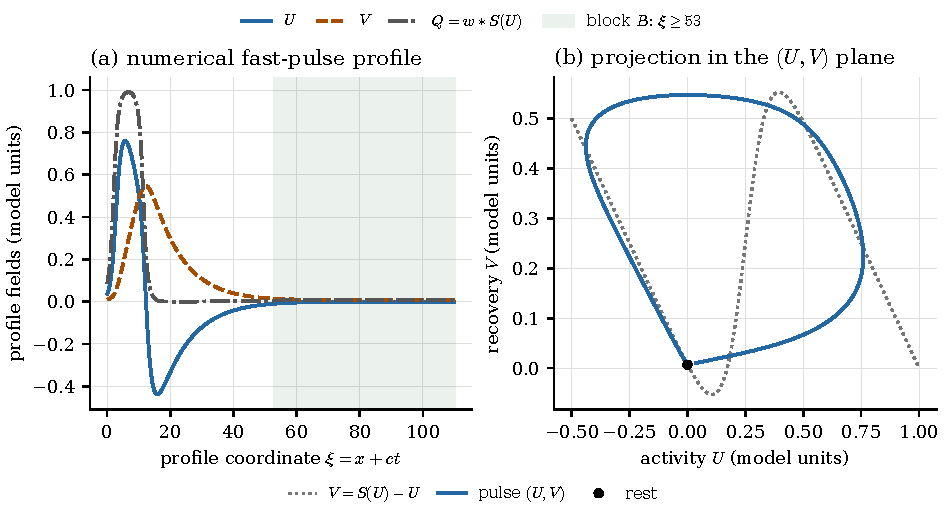
\includegraphics[width=\textwidth]{figures/pulse-profile.pdf}
\caption{The fast pulse of Theorem~\ref{thm:fast}, computed numerically at a speed within $10^{-55}$ of the speed $c_*$ of Section~\ref{sec:numerics} (\texttt{code/orbit\_hp.py}, \texttt{code/figure.py}). Left: $U$, $V$ and $Q = w * S(U)$ against $\xi$, with $\xi = 0$ at the manifold point $\Phi_{1/c}(1/4)$; the shaded range is where the proof keeps the orbit in the block $B$. Right: the orbit in the $(U, V)$ plane, drawn from $\xi = 0$ (the short piece on the unstable manifold between the rest state and $\Phi_{1/c}(1/4)$ is not drawn), with the curve $V = S(U) - U$, the nullcline of the space-clamped equation $u_t = -u - v + S(u)$.}\label{fig:profile}
\end{figure}

\section{Reproducibility}\label{sec:reproduce}

The programs need Python $3.11$ with the packages of \file{code/requirements.txt} (python-flint $0.9.0$, \texttt{mpmath} $1.3.0$, \texttt{numpy} $2.4.6$, \texttt{matplotlib} $3.11.2$ for the figure, SymPy $1.14.0$ for \file{part3_symbolic.py} and SciPy $1.17.1$ for the numerical scripts). From the folder of this paper (times are wall-clock times on the four-core machine used for this paper, which was busy with other work):

{\small
\begin{longtable}{@{}>{\raggedright\arraybackslash}p{0.44\textwidth}>{\raggedright\arraybackslash}p{0.49\textwidth}@{}}
\toprule
command & what it proves, and time \\
\midrule
\endhead
\texttt{sh code/run\_all.sh} & Theorem~\ref{thm:fast}: the $20$ checks of Table~\ref{tab:checks}, whose committed output is \file{data/run_all.txt}; about $6$ min with the steps that the script runs in parallel run one after another \\
\texttt{sh ext/slow-pulse/code/run\_all.sh} & Theorem~\ref{thm:slow}: $26$ checks, about $1$ min with its parallel steps run one after another \\
\texttt{sh ext/gain-12/code/run\_all.sh} & Theorem~\ref{thm:gain12}: $23$ checks, about $3$ min with its parallel steps run one after another \\
\texttt{sh ext/faye-model/code/run\_all.sh 1/20} (and \texttt{1/50}, \texttt{1/100}) & Theorem~\ref{thm:faye}: $14$ checks each; about $4$, $12$ and $49$ min with the parallel steps run one after another \\
\texttt{sh ext/eps-range/run\_checks.sh} & Theorem~\ref{thm:range}: tests, one interval proved from scratch with its negative controls, the coverage of $[0.08, 0.13693]$ by the stored certificates and the acceptance of those in \file{ext/eps-range/data/probes/}; about $2$ min with its four chain runs run one after another \\
\texttt{python3 ext/eps-range/table.py -{}-from 0.08 -{}-to 0.13693 -{}-condensed -{}-at 1/10} & the coverage, Table~\ref{tab:range} and the window at $\eps = 1/10$ (\file{ext/eps-range/data/table_summary.txt}); \texttt{-{}-certs ext/eps-range/data/probes -{}-at 3/20} gives the four accepted probes, three of which are further intervals of $\mathcal{E}$, and the window at $\eps = 3/20$ (\file{ext/eps-range/data/probe_summary.txt}); seconds \\
\texttt{python3 ext/eps-range/run\_range.py 0.08 0.13693 -{}-w0 1.5e-4} & a new sweep of $[0.08, 0.13693]$, once the stored certificates are moved away (the program skips an attempt that has one); it may choose other subintervals than the stored ones; about four hours on four cores. The arguments \texttt{0.138 0.1382} and \texttt{0.1395 0.1397} recompute the two further certificates of \file{ext/eps-range/data/certs/}, and \texttt{bash ext/eps-range/probe\_limits.sh} the single attempts of \file{ext/eps-range/data/probes/} \\
\texttt{sh ext/stability/run\_all.sh quick} & Theorem~\ref{thm:stab} without recomputing the winding pieces or the pieces of the controls: the $15$ checks of Table~\ref{tab:stabchecks}, whose committed output is \file{ext/stability/data/run_all.txt}; about $26$ min with its parallel steps run one after another, most of it \texttt{simple\_zero.py}, then about $20$ min of numerical scripts \\
\texttt{sh ext/stability/run\_all.sh} & the same with the six winding pieces, $16$ to $31$ min each on four cores, and the four pieces of the controls, which took $2.5$ to $10.5$ min each on one core (the script runs them with four workers) \\
\bottomrule
\end{longtable}}

\medskip
Each script prints one line per check and exits with status $1$ if a proof step fails or a negative control passes. Every script refuses to run when \texttt{PYTHONOPTIMIZE} is set and clears every \texttt{NF\_*} environment variable, since the first would remove the Python assertions that some programs still use as gates and the second change parameters, blocks, precision, order or tolerances (Section~\ref{sec:limits}). On 2026-09-27 each script of this table except \texttt{run\_range.py} and \texttt{probe\_limits.sh} was rerun from a copy of the folder, one process at a time and with twelve \texttt{NF\_*} variables set in the environment (the stability script with the argument \texttt{quick}), and \texttt{winding\_controls.py run} recomputed the four pieces of the controls: every check passed, and every summary, certificate and piece is identical to the committed one apart from timing fields. Later that day the programs changed only by the refusal of \texttt{python -O} at import, the prelude of \texttt{run\_range.py} and docstrings; the scripts were then rerun in the same way with the present programs, with the same result. Of the computations that the scripts do not repeat, two of the six winding pieces, the one that passes closest to the zero $\lambda = 0$ (the lower half of the left side of $\partial\Rbox$) and the top side, where $|\lambda|$ is largest, were recomputed and are identical to the stored pieces apart from their times, segment by segment; and nineteen of the accepted certificates of Theorem~\ref{thm:range}, among them the one that contains $\eps = 1/10$ and the four accepted probes, were recomputed with the present programs: all nineteen passed, with the same rest state, manifold validation and block, the same number of stages, the same block entry time and all in-run negative checks refused; three are identical to the stored ones, and the other sixteen differ only in numerically chosen data of the stages of the covering chain, because a rerun takes the numerical pulse data from a stored table rather than recomputing them from an unrecorded speed guess. The details, and the argument for the computations that were not repeated, are in \file{review/RERUNS.md}. Each piece of the winding number, and each piece of its controls, records the SHA-256 digests of \file{ext/stability/evans_rig.py}, \file{ext/stability/winding.py} and \file{ext/stability/data/pulse_records.pkl}, and \texttt{winding.py combine} and \texttt{winding\_controls.py check} refuse the pieces unless these equal the digests of the present files. The base modules that \file{evans_rig.py} imports are not fingerprinted: \file{code/nfcore.py} ($S$, $S'$ and the Taylor recursion of the pulse), \file{code/certify_rest.py} ($c_1$ and $c_2$, which set the range of $\kappa$ of the smaller block) and \file{code/block.py} (the check of the smaller block). Since the pieces were computed (commit \texttt{5af378b}), \file{certify_rest.py} and \file{block.py} have changed only in comments, and \file{nfcore.py} only by the refusal of \texttt{python -O} (Section~\ref{sec:limits}). The files of the proofs of Theorems~\ref{thm:fast} and~\ref{thm:stab} have the following SHA-256 prefixes (the full digests of \file{evans_rig.py}, \file{winding.py} and the pulse records are in \file{ext/stability/data/winding.json}, and \texttt{sha256sum} prints all of them); the certificates of Theorem~\ref{thm:range} record the prefixes of the programs that made them (Section~\ref{sec:proof-range}):

\medskip
{\footnotesize
\begin{tabular}{@{}ll@{\qquad}ll@{}}
\toprule
in \texttt{code/} & SHA-256, first 16 digits & in \texttt{ext/stability/} & SHA-256, first 16 digits \\
\midrule
\texttt{nfcore.py} & \texttt{0bfb2bab95a8ed49} & \texttt{ess\_spectrum.py} & \texttt{eec6864605a1c4ca} \\
\texttt{certify\_rest.py} & \texttt{000acf9bb8641ef1} & \texttt{large\_lambda.py} & \texttt{0a06600a22c438df} \\
\texttt{manifold.py} & \texttt{a5a4d66b38c01a2e} & \texttt{pulse\_enclosure.py} & \texttt{f23d581eed4ac73b} \\
\texttt{block.py} & \texttt{01d5d81f89a0ae99} & \texttt{simple\_zero.py} & \texttt{e12cb36b56559933} \\
\texttt{block\_check\_iv.py} & \texttt{91fcda1c252b7652} & \texttt{part3\_symbolic.py} & \texttt{9a81eb57f7f47499} \\
\texttt{lohner.py} & \texttt{3746e2320017f015} & \texttt{evans\_rig.py} & \texttt{0057267d1af27862} \\
\texttt{prove\_pulse.py} & \texttt{8bf63203b2646b95} & \texttt{winding.py} & \texttt{93b17f170e546f2e} \\
\texttt{run\_all.sh} & \texttt{be792b0024bb7a1e} & \texttt{data/pulse\_records.pkl} & \texttt{7e2bdbbdc8fa4e31} \\
\bottomrule
\end{tabular}}

\section{Limitations and what has been checked}\label{sec:limits}

\paragraph{Nonlinear stability is not proved.} Theorem~\ref{thm:stab} is a statement about the spectrum. Sandstede \cite{sandstede2007} proves, according to its abstract, that spectral stability implies nonlinear stability for traveling waves of neuronal network models in appropriate function spaces \cite[p.~2693]{sandstede2007}. We have not read that paper, and the secondary sources disagree on its scope: Faye invokes it for a smooth firing rate (``the results for neural field equations of Sandstede'' \cite[p.~17 of the author's copy]{faye2013}) but lists it among the studies in which the firing rate is a Heaviside function \cite[p.~2]{faye2013}, and Dyson describes it as proving ``that spectral stability implies nonlinear stability for neural field models with single Heaviside firing rates'' \cite[p.~29]{dyson2018}. Whether its hypotheses cover \eqref{eq:field} with $\gamma = 0$, the exponential kernel and a logistic rate, and whether its function spaces match $X$, is therefore unknown. The nearest proved principle of linearized stability that we found, that of Habib and Veltz \cite[Theorem~1, p.~7]{hv2024}, is for a Wilson--Cowan field with the firing rate outside the convolution and does not apply to \eqref{eq:field} as stated; they note that the principle had been conjectured \cite[p.~2]{hv2024}. A self-contained proof would need at least: that $\Lop$ generates a $C_0$-group on $X$, that $e^{t\Lop} - e^{t\Lop_\infty}$ is compact, so that the essential growth bound is that of the Fourier multiplier group, and a modulation argument for the translation mode. None of this is done here.

\paragraph{The class $\Pcl$ and Theorem~\ref{thm:fast}.} Theorem~\ref{thm:stab} covers the pulses of $\Pcl$, with speed in a bracket of width $10^{-58}$ and in the block from $\xi = 110$; a pulse of $\Pcl$ satisfies all conclusions of Theorem~\ref{thm:fast} (Section~\ref{sec:results}). Whether every pulse with speed in $(c_1, c_2)$ that leaves the rest state on the branch on which $U$ increases is one of them, and in particular the pulse given by the proof of Theorem~\ref{thm:fast}, would follow from uniqueness of such a pulse, which is not proved, or from a stability computation over the whole bracket of Theorem~\ref{thm:fast}, for which the enclosure of the pulse beyond $\xi = 53$ is too wide with the present method. No theorem here concerns uniqueness, except that Corollary~\ref{cor:two} shows that there are at least two pulses at $\eps = 1/10$ and at $\eps = 3/20$; nothing is proved about the stability of the slow pulses, of the pulses of Theorems~\ref{thm:range}, \ref{thm:gain12} and~\ref{thm:faye}, or about other parameter values.

\paragraph{What has been checked.} The following checks were made within the project by separate AI agent sessions, each instructed to find errors and each with its report in the folder. For Theorem~\ref{thm:fast}: a reading of the mathematics that wrote out the arguments now in Section~\ref{sec:existence} (\file{review/lead/math/MATH.md}); an audit of the code with $32$ mutations (\file{review/lead/code/CODE.md}); a reimplementation from the equations alone, with its own validated integrator, its own block in exact rational arithmetic and its own shooting argument, which proves the existence step again (\file{review/lead/reimpl/}); a check of the earlier literature (\file{review/lead/priorart/PRIORART.md}); and a concurrent second review of the same kind (\file{review/}). Their must-fix findings are fixed in the programs, and \file{review/lead/VERIFY.md} lists the fixes. Theorems~\ref{thm:range}--\ref{thm:faye} each had one adversarial check that reran the chain from a copy, recomputed decisive numbers with its own code and ran mutation tests (the \texttt{REPORT.md} of each folder under \file{ext/}). For Theorem~\ref{thm:stab}, one adversarial check reran and recomputed the essential spectrum, the exclusion of large eigenvalues, the pulse enclosure and several thin Evans enclosures with its own code, and found no error; it predates the winding number and the Cauchy integral, which it did not rerun, and a local rerun of four of the six winding pieces gave the same intervals (\file{ext/stability/REPORT.md}, Section~1). Three separate agent sessions checked the completeness, the claims and the literature of a first draft of this paper against the folder, and the findings confirmed there were applied. The revised manuscript then had three readings on 2026-09-27, again by separate AI agent sessions within the project, each instructed to find errors and each with one lens: the analysis (every written proof read line by line), the computation (the check scripts of Theorems~\ref{thm:fast}, \ref{thm:range}, \ref{thm:slow} and~\ref{thm:gain12} and the steps of Theorem~\ref{thm:stab}, except the six winding pieces, rerun from a copy, and the printed numbers traced to the outputs; the chains of Theorem~\ref{thm:faye} were not rerun) and the claims and the literature (the quotations and references checked in the sources that could be reached). Every finding was examined by two further agent sessions; the confirmed ones are fixed in this version. The passages written in response (Lemma~\ref{lem:fayemanifold} with the embedding of Faye's model, the corrected step of the proof of Lemma~\ref{lem:branch}, Lemma~\ref{lem:multiplicity} and the statements about the class $\Pcl$), with the Fredholm step of Proposition~\ref{prop:ess}, the proof of the Krawczyk test in Section~\ref{sec:method} and the citations of Teschl, had a fourth reading the same day, by a separate agent session briefed only with the paper, its programs and excerpts of the two cited books. It found no error that makes a proof wrong or a statement false; the fuller arguments it asked for (that the parametrized curve is the local unstable manifold in Lemma~\ref{lem:branch}, the boundedness of $z_1$ in Lemma~\ref{lem:multiplicity}, and the argument for $\xi \ge 120$ in Lemma~\ref{lem:class}(b)) are in this version. A fifth, narrow reading of those passages found no error, and the three clauses it asked for are added. The controls W1, W2 and Z3 of Table~\ref{tab:stabchecks} had a review of their own, which found that they do what they are said to do, found one wrong statement about how the pieces of W1 and W2 were computed (now corrected), and asked for the statements about them now in Sections~\ref{sec:stability}, \ref{sec:method} and~\ref{sec:reproduce}. The reports, with the response to each finding, are kept with the quality record of the paper, outside this folder. The readings do not replace a check of Arb or of the Python interpreter, and the mutation study shows that the automatic checks cannot detect every loss of rigor in the integrator (Section~\ref{sec:method}).

\paragraph{Program hygiene.} The base programs enforce every rigorous gate with an explicit check. Some programs of the extensions and of the stability proof use Python \texttt{assert} statements for gates of the proof, for example the manifold validation in \file{ext/stability/pulse_enclosure.py}, the certification of the smaller block and a consistency check of the eigenvalue enclosures in \file{ext/stability/evans_rig.py}, the refusal by \texttt{winding.py combine} of pieces with other SHA-256 digests and its check that the pieces close the path, the manifold and block checks of the drivers in \file{ext/gain-12/code/}, \file{ext/faye-model/code/} and \file{ext/eps-range/chain.py} (including the positivity of the time rescaling in \file{lohner7.py}), and the check of the range of $\eps_0$ in \file{ext/eps-range/table.py}. A failed assertion stops the program, as an explicit check does, but Python removes assertions when it runs with \texttt{-O} or with \texttt{PYTHONOPTIMIZE} set. Every program of this folder therefore refuses to run in that case: the modules that the programs import (\file{code/nfcore.py}, its copy in \file{ext/gain-12/code/}, \file{ext/faye-model/code/fcore.py} and \file{ext/stability/_paths.py}) and the programs that import none of them (the two \texttt{mpmath} re-checks of the blocks, \file{ext/eps-range/table.py} and \file{run_range.py}) exit at once under \texttt{-O}, so an assertion is active whenever a program runs; each program that contains an \texttt{assert} statement was started with \texttt{-O} and stopped at once. Every check script, and \file{run_range.py}, also clears every \texttt{NF\_*} environment variable. The variables matter: besides \texttt{NF\_EVANS\_*} and \texttt{NF\_STAB\_*} (precision, order and tolerances of \file{evans_rig.py} and \file{pulse_enclosure.py}), the stability programs read, through the base modules they import, \texttt{NF\_PULSE} (which switches $c_1$ and $c_2$ in \file{code/certify_rest.py}, and with them the speed bound of \file{large_lambda.py} and the range of $\kappa$ of the smaller block), \texttt{NF\_DU} and \texttt{NF\_R\_OVER\_RHO} (the block $B$ in \file{code/prove_pulse.py}), and \texttt{NF\_PREC}, \texttt{NF\_TOL}, \texttt{NF\_ORDER} and \texttt{NF\_TAG}; the programs of \file{ext/gain-12/code/} read \texttt{NF\_BETA} and \texttt{NF\_EPS}, and \file{ext/eps-range/chain.py} several more. A program run on its own, outside its script, must be run without any \texttt{NF\_*} variable, as the committed runs were.

\paragraph{Sources.} The published results that a proof here uses are taken from sources we read: the local unstable manifold theorem, the continuity of the flow and global existence under linear growth from Teschl \cite[Theorems~9.4, 9.5, 6.1 and~2.17]{teschl2012}; the analytic Fredholm theory from Dyatlov and Zworski \cite[Appendix~C, Theorems~C.5, C.8 and~C.9]{dz2019}; and the Krawczyk test from Rump \cite[Theorem~13.3]{rump2010}. Of Zhang \cite{zhang2004} we read pp.~162--165 (the abstract, the model with the Heaviside rate, Theorem~1), pp.~168--171 and~186 (the plan for pulses) and p.~194 (Theorems~3 and~4, on pulses of the singularly perturbed Heaviside system for sufficiently small $\eps$, stated with their proofs deferred to other papers), and searched the rest for the firing rate and for pulses. We could not reach the full texts of seven works. We read: Zhang \cite{zhang2005}, pp.~489--490 and its zbMATH review (Zbl 1082.45009); Zhang \cite{zhang2007}, pp.~283--284; Zhang \cite{zhang2004acta}, pp.~283--284; Zhang \cite{zhang2007siads}, its abstract; Pinto, Jackson and Wayne \cite{pjw2005}, the abstract and Dyson's account \cite[pp.~7--8]{dyson2025}; and Sandstede \cite{sandstede2007}, the abstract. Every page of these that we reached uses the Heaviside rate or concerns stability: \cite{zhang2004} treats fronts of a scalar Heaviside equation, \cite{zhang2005} the Heaviside system for $\eps = 0$ and $0 < \eps \ll 1$, \cite{zhang2007} fronts of a scalar Heaviside equation and standing waves of the forced system, and \cite{zhang2004acta} the stability of fast pulses. Faye lists \cite{zhang2005}, \cite{pjw2005}, \cite{sandstede2007}, \cite{zhang2007siads}, whose abstract concerns traveling waves of a nonlocal model with spatio-temporal delay, and a paper cited with the title of \cite{zhang2004} and the journal of another Zhang paper among the studies in which the firing rate is a Heaviside function \cite[p.~2 and references~33, 35 and~42--44]{faye2013}. Enculescu \cite{enculescu2004} is unread, and we know nothing of its contents beyond its title and the contexts in which it is cited, which suggest a Heaviside or high-gain construction. Coombes and Owen \cite{co2004} was read in the authors' preprint (\file{ext/stability/REPORT.md}). Of Ermentrout, Jalics and Rubin \cite{ejr2010} we read, in an author-posted copy, the abstract, Sections~1, 2.1, 3 (its opening and Section~3.1) and~4: its rigorous result concerns fronts locked to a small stimulus, and its treatment of pulses assumes a pulse of the unstimulated field with slow recovery. Of Ermentrout and McLeod \cite{em1993} we read pp.~461--462 (the synopsis, the model and its hypotheses) in an author-posted scan. The statements about earlier work in Section~\ref{sec:intro} are limited accordingly: they say what the works we read contain, and they name the works we could not read.

\section{Discussion}\label{sec:discussion}

The existence results for smooth firing rates that we found are asymptotic in $\eps$, or conditional on hypotheses checked only numerically or not at all (Section~\ref{sec:intro}). Theorems~\ref{thm:fast}--\ref{thm:faye} replace the limit $\eps \to 0$ by a rigorous computation at a given $\eps$: the orbit is followed in ball arithmetic from a validated piece of the unstable manifold to a block around the rest state, and closed there by a topological argument in the speed. The price is that each theorem holds at the parameter values computed, and that the enclosures must survive the strong sensitivity of the orbit to the speed; at $\eps = 1/100$ in Faye's model this takes a bracket of $144$ digits. For a range of $\eps$ the covering relations of Theorem~\ref{thm:range} reset the enclosure every unit of time, which makes each interval of $\eps$ cheap, but the chain stops where the back of the pulse barely expands the unstable direction (numerically, Section~\ref{sec:numerics}).

The pulses found agree with the picture Pinto and Ermentrout drew for the Heaviside rate \cite[Sect.~3.1]{pe2001}: a fast and a slow pulse coexist at $\eps = 1/10$ and at $\eps = 3/20$ (Corollary~\ref{cor:two}), and the numerical continuation of the fast branch loses its bracket between $\eps = 0.220$ and $0.225$, as at a fold where the two meet (numerical, Section~\ref{sec:numerics}). They expected the fast pulse to be stable and the slow one unstable \cite[Sect.~3.1]{pe2001}. Theorem~\ref{thm:stab} proves the first half at the spectral level, for the class $\Pcl$ at $\eps = 1/10$, and the direct simulation of the field (Section~\ref{sec:numerics}) is attracted to that pulse from several stimuli, which is what nonlinear stability would explain. The rest state is a saddle-focus in Theorem~\ref{thm:gain12}, where this is certified, and, numerically, in Theorem~\ref{thm:slow}(b); in both the block is built in a real Jordan basis, with a Lyapunov form in Theorem~\ref{thm:gain12}, and the complex eigenvalues are not an obstacle to the method.

\section{Open problems}\label{sec:open}

\begin{enumerate}
\item Are the pulses of $\Pcl$ in Theorem~\ref{thm:stab} nonlinearly (orbitally) stable? Sandstede's theorem \cite{sandstede2007} may settle it, if its hypotheses cover \eqref{eq:field}; otherwise a principle of linearized stability for \eqref{eq:field}, in the spirit of \cite{hv2024}, is needed: a $C_0$-group on $X$, the compactness of $e^{t\Lop} - e^{t\Lop_\infty}$ and a modulation argument (Section~\ref{sec:limits}).
\item Is every pulse with speed in $(c_1, c_2)$ that leaves the rest state on the branch on which $U$ increases in the class $\Pcl$? A proof that such a pulse is unique would give it, and so would a stability computation over the whole bracket of Theorem~\ref{thm:fast}, which needs a sharper enclosure of the pulse beyond $\xi = 53$.
\item Are the slow pulses of Theorem~\ref{thm:slow} unstable, with exactly one positive eigenvalue, as Pinto and Ermentrout expect? An Evans-function count as in Section~\ref{sec:stability}, on a box that contains the expected unstable eigenvalue, might settle this. The stability of the pulses of Theorems~\ref{thm:range}, \ref{thm:gain12} and~\ref{thm:faye} is open as well.
\item Can the range of $\eps$ be extended? Below $0.07$ the weakest stable eigenvalue of the rest state is small and the chains are long; near $\eps = 0.176$ two stable eigenvalues become complex, which calls for the block in a real Jordan basis used for Theorem~\ref{thm:gain12}; and near $0.22$ the fast and slow pulses appear to meet in a fold, which a proof would have to follow through its turning point.
\item At gain $12$ the unstable eigenvalue exceeds the modulus of the real part of the complex pair (R5, certified). If the homoclinic orbit of Theorem~\ref{thm:gain12} is also shown to be transversal in the parameter $c$, Shilnikov's theory gives multi-pulses accumulating on it, which the shooting finds numerically (Section~\ref{sec:numerics}). Can this be proved?
\item Hastings asks for an existence proof that covers all reasonable smooth firing rates \cite[p.~2]{hastings2017}. Can the computations be continued in the gain $\beta$, or in $\theta$, to cover a family of smooth rates at fixed $\eps$? In Faye's model, does the slow pulse exist at his parameters, and do Hastings's hypotheses hold at $(\eps, c_1) = (0.005, 0.34)$?
\end{enumerate}

\medskip
{\raggedright\noindent\textbf{Data availability.} The programs of this paper and their output are in its folder: the base proof in \texttt{code/} and \texttt{data/}, the extensions in \texttt{ext/slow-pulse/}, \texttt{ext/gain-12/}, \texttt{ext/eps-range/}, \texttt{ext/faye-model/} and \texttt{ext/stability/}, each with a report, and the project's checks in \texttt{review/}. A public release of that folder with an archived DOI is planned before submission.\par}

\noindent\textbf{Funding.} This research received no external funding.

\smallskip
\noindent{\footnotesize This work was prepared with AI assistance. The author takes full responsibility for its content.}

\begin{thebibliography}{40}
\small

\bibitem{agj1990} J. Alexander, R. Gardner and C. Jones, A topological invariant arising in the stability analysis of travelling waves, \emph{J. Reine Angew. Math.} \textbf{410} (1990) 167--212; doi:10.1515/crll.1990.410.167.

\bibitem{amari1977} S. Amari, Dynamics of pattern formation in lateral-inhibition type neural fields, \emph{Biol. Cybern.} \textbf{27} (1977) 77--87; doi:10.1007/BF00337259.

\bibitem{ak2015} G. Arioli and H. Koch, Existence and stability of traveling pulse solutions of the FitzHugh--Nagumo equation, \emph{Nonlinear Anal.} \textbf{113} (2015) 51--70; doi:10.1016/j.na.2014.09.023.

\bibitem{bz2016} B. Barker and K. Zumbrun, Numerical proof of stability of viscous shock profiles, \emph{Math. Models Methods Appl. Sci.} \textbf{26} (2016) 2451--2469; doi:10.1142/S0218202516500585.

\bibitem{bressloff2012} P. C. Bressloff, Spatiotemporal dynamics of continuum neural fields, \emph{J. Phys. A} \textbf{45} (2012) 033001; doi:10.1088/1751-8113/45/3/033001.

\bibitem{bop2025} E. Burlakov, A. Oleynik and A. Ponosov, Travelling waves in neural fields with continuous and discontinuous neuronal activation, \emph{Mathematics} \textbf{13} (2025) 701; doi:10.3390/math13050701.

\bibitem{cfl2003} X. Cabr\'e, E. Fontich and R. de la Llave, The parameterization method for invariant manifolds I: Manifolds associated to non-resonant subspaces, \emph{Indiana Univ. Math. J.} \textbf{52} (2003) 283--328; doi:10.1512/iumj.2003.52.2245.

\bibitem{conley1978} C. Conley, \emph{Isolated Invariant Sets and the Morse Index}, CBMS Regional Conference Series in Mathematics \textbf{38}, American Mathematical Society, Providence, RI, 1978.

\bibitem{co2004} S. Coombes and M. R. Owen, Evans functions for integral neural field equations with Heaviside firing rate function, \emph{SIAM J. Appl. Dyn. Syst.} \textbf{3} (2004) 574--600; doi:10.1137/040605953.

\bibitem{dz2019} S. Dyatlov and M. Zworski, \emph{Mathematical Theory of Scattering Resonances}, Graduate Studies in Mathematics \textbf{200}, American Mathematical Society, Providence, RI, 2019; Appendix~C is cited from the authors' version~1.0 of August~19, 2022, posted at \url{https://math.mit.edu/~dyatlov/res/}.

\bibitem{dyson2018} A. Dyson, Existence of traveling fronts and pulses in lateral inhibition neuronal networks with sigmoidal firing rate functions, preprint, arXiv:1810.05142v1 (2018), whose page numbers are cited. A revised version, retitled for fronts, is \emph{SIAM J. Appl. Dyn. Syst.} \textbf{19} (2020) 2194--2231; doi:10.1137/20M1311697.

\bibitem{dyson2025} A. Dyson, Existence and uniqueness of fast traveling pulses in singularly perturbed nonlocal neural fields with Heaviside nonlinearities: a complete proof, preprint, arXiv:2511.17328v2 (2025), whose page numbers are cited.

\bibitem{enculescu2004} M. Enculescu, A note on traveling fronts and pulses in a firing rate model of a neuronal network, \emph{Physica D} \textbf{196} (2004) 362--386; doi:10.1016/j.physd.2004.06.005.

\bibitem{ejr2010} G. B. Ermentrout, J. Z. Jalics and J. E. Rubin, Stimulus-driven traveling solutions in continuum neuronal models with a general smooth firing rate function, \emph{SIAM J. Appl. Math.} \textbf{70} (2010) 3039--3064; doi:10.1137/090775737.

\bibitem{em1993} G. B. Ermentrout and J. B. McLeod, Existence and uniqueness of travelling waves for a neural network, \emph{Proc. Roy. Soc. Edinburgh Sect. A} \textbf{123} (1993) 461--478; doi:10.1017/S030821050002583X.

\bibitem{faye2013} G. Faye, Existence and stability of traveling pulses in a neural field equation with synaptic depression, \emph{SIAM J. Appl. Dyn. Syst.} \textbf{12} (2013) 2032--2067; doi:10.1137/130913092. Pages are cited from the author's copy dated September 5, 2013.

\bibitem{fs2015} G. Faye and A. Scheel, Existence of pulses in excitable media with nonlocal coupling, \emph{Adv. Math.} \textbf{270} (2015) 400--456; doi:10.1016/j.aim.2014.11.005; arXiv:1311.6508v1, whose page numbers are cited.

\bibitem{hv2024} S. Habib and R. Veltz, Theoretical / numerical study of modulated traveling waves in inhibition stabilized networks, preprint, arXiv:2412.03613v1 (2024), whose printed page numbers are cited.

\bibitem{hastings2017} S. P. Hastings, Existence of travelling pulses in a neural model, \emph{Proc. Roy. Soc. Edinburgh Sect. A} \textbf{147} (2017) 397--427; doi:10.1017/S0308210516000044; arXiv:1503.04057v2, whose page numbers are cited.

\bibitem{johansson2017} F. Johansson, Arb: efficient arbitrary-precision midpoint-radius interval arithmetic, \emph{IEEE Trans. Comput.} \textbf{66} (2017) 1281--1292; doi:10.1109/TC.2017.2690633.

\bibitem{capd2021} T. Kapela, M. Mrozek, D. Wilczak and P. Zgliczy\'nski, CAPD::DynSys: a flexible C++ toolbox for rigorous numerical analysis of dynamical systems, \emph{Commun. Nonlinear Sci. Numer. Simul.} \textbf{101} (2021) 105578; doi:10.1016/j.cnsns.2020.105578.

\bibitem{kp2013} T. Kapitula and K. Promislow, \emph{Spectral and Dynamical Stability of Nonlinear Waves}, Applied Mathematical Sciences \textbf{185}, Springer, New York, 2013; doi:10.1007/978-1-4614-6995-7.

\bibitem{krawczyk1969} R. Krawczyk, Newton-Algorithmen zur Bestimmung von Nullstellen mit Fehlerschranken, \emph{Computing} \textbf{4} (1969) 187--201; doi:10.1007/BF02234767.

\bibitem{lohner1987} R. J. Lohner, Enclosing the solutions of ordinary initial and boundary value problems, in: E. Kaucher, U. Kulisch and Ch. Ullrich (eds.), \emph{Computer Arithmetic: Scientific Computation and Programming Languages}, Teubner, Stuttgart, 1987, pp.~255--286.

\bibitem{sympy} A. Meurer et al., SymPy: symbolic computing in Python, \emph{PeerJ Comput. Sci.} \textbf{3} (2017) e103; doi:10.7717/peerj-cs.103.

\bibitem{mpmath} The mpmath development team, \emph{mpmath: a Python library for arbitrary-precision floating-point arithmetic}, version 1.3.0 (2023), \url{https://mpmath.org}.

\bibitem{pe2001} D. J. Pinto and G. B. Ermentrout, Spatially structured activity in synaptically coupled neuronal networks: I. Traveling fronts and pulses, \emph{SIAM J. Appl. Math.} \textbf{62} (2001) 206--225; doi:10.1137/S0036139900346453.

\bibitem{pjw2005} D. J. Pinto, R. K. Jackson and C. E. Wayne, Existence and stability of traveling pulses in a continuous neuronal network, \emph{SIAM J. Appl. Dyn. Syst.} \textbf{4} (2005) 954--984; doi:10.1137/040613020.

\bibitem{rump2010} S. M. Rump, Verification methods: rigorous results using floating-point arithmetic, \emph{Acta Numer.} \textbf{19} (2010) 287--449; doi:10.1017/S096249291000005X.

\bibitem{sandstede2007} B. Sandstede, Evans functions and nonlinear stability of traveling waves in neuronal network models, \emph{Internat. J. Bifur. Chaos} \textbf{17} (2007) 2693--2704; doi:10.1142/S0218127407018695.

\bibitem{teschl2012} G. Teschl, \emph{Ordinary Differential Equations and Dynamical Systems}, Graduate Studies in Mathematics \textbf{140}, American Mathematical Society, Providence, RI, 2012; theorem numbers are those of the author's version of April~2012, posted with the publisher's permission at \url{https://www.mat.univie.ac.at/~gerald/ftp/book-ode/}.

\bibitem{tucker2011} W. Tucker, \emph{Validated Numerics: A Short Introduction to Rigorous Computations}, Princeton University Press, Princeton, NJ, 2011.

\bibitem{bmlm2011} J. B. van den Berg, J. D. Mireles James, J.-P. Lessard and K. Mischaikow, Rigorous numerics for symmetric connecting orbits: even homoclinics of the Gray--Scott equation, \emph{SIAM J. Math. Anal.} \textbf{43} (2011) 1557--1594; doi:10.1137/100812008.

\bibitem{wazewski1947} T. Wa\.zewski, Sur un principe topologique de l'examen de l'allure asymptotique des int\'egrales des \'equations diff\'erentielles ordinaires, \emph{Ann. Soc. Polon. Math.} \textbf{20} (1947) 279--313.

\bibitem{wz2003} D. Wilczak and P. Zgliczy\'nski, Heteroclinic connections between periodic orbits in planar restricted circular three-body problem---a computer assisted proof, \emph{Comm. Math. Phys.} \textbf{234} (2003) 37--75; doi:10.1007/s00220-002-0709-0.

\bibitem{z2009} P. Zgliczy\'nski, Covering relations, cone conditions and the stable manifold theorem, \emph{J. Differential Equations} \textbf{246} (2009) 1774--1819; doi:10.1016/j.jde.2008.12.019.

\bibitem{zg2004} P. Zgliczy\'nski and M. Gidea, Covering relations for multidimensional dynamical systems, \emph{J. Differential Equations} \textbf{202} (2004) 32--58; doi:10.1016/j.jde.2004.03.013.

\bibitem{zhang2004} L. Zhang, Existence, uniqueness and exponential stability of traveling wave solutions of some integral differential equations arising from neuronal networks, \emph{J. Differential Equations} \textbf{197} (2004) 162--196; doi:10.1016/S0022-0396(03)00170-0.

\bibitem{zhang2004acta} L. Zhang, Exponential stability of traveling pulse solutions of a singularly perturbed system of integral differential equations arising from excitatory neuronal networks, \emph{Acta Math. Appl. Sin. Engl. Ser.} \textbf{20} (2004) 283--308; doi:10.1007/s10255-004-0168-9.

\bibitem{zhang2005} L. Zhang, Traveling waves of a singularly perturbed system of integral-differential equations arising from neuronal networks, \emph{J. Dynam. Differential Equations} \textbf{17} (2005) 489--522; doi:10.1007/s10884-005-5404-3.

\bibitem{zhang2007} L. Zhang, Dynamics of neuronal waves, \emph{Math. Z.} \textbf{255} (2007) 283--321, published online 29 July 2006; doi:10.1007/s00209-006-0024-0.

\bibitem{zhang2007siads} L. Zhang, How do synaptic coupling and spatial temporal delay influence traveling waves in nonlinear nonlocal neuronal networks?, \emph{SIAM J. Appl. Dyn. Syst.} \textbf{6} (2007) 597--644; doi:10.1137/06066789X.

\end{thebibliography}

\end{document}
